\documentclass[twoside]{book}

% Packages required by doxygen
\usepackage{fixltx2e}
\usepackage{calc}
\usepackage{doxygen}
\usepackage{graphicx}
\usepackage[utf8]{inputenc}
\usepackage{makeidx}
\usepackage{multicol}
\usepackage{multirow}
\PassOptionsToPackage{warn}{textcomp}
\usepackage{textcomp}
\usepackage[nointegrals]{wasysym}
\usepackage[table]{xcolor}

% Font selection
\usepackage[T1]{fontenc}
\usepackage{mathptmx}
\usepackage[scaled=.90]{helvet}
\usepackage{courier}
\usepackage{amssymb}
\usepackage{sectsty}
\renewcommand{\familydefault}{\sfdefault}
\allsectionsfont{%
  \fontseries{bc}\selectfont%
  \color{darkgray}%
}
\renewcommand{\DoxyLabelFont}{%
  \fontseries{bc}\selectfont%
  \color{darkgray}%
}
\newcommand{\+}{\discretionary{\mbox{\scriptsize$\hookleftarrow$}}{}{}}

% Page & text layout
\usepackage{geometry}
\geometry{%
  a4paper,%
  top=2.5cm,%
  bottom=2.5cm,%
  left=2.5cm,%
  right=2.5cm%
}
\tolerance=750
\hfuzz=15pt
\hbadness=750
\setlength{\emergencystretch}{15pt}
\setlength{\parindent}{0cm}
\setlength{\parskip}{0.2cm}
\makeatletter
\renewcommand{\paragraph}{%
  \@startsection{paragraph}{4}{0ex}{-1.0ex}{1.0ex}{%
    \normalfont\normalsize\bfseries\SS@parafont%
  }%
}
\renewcommand{\subparagraph}{%
  \@startsection{subparagraph}{5}{0ex}{-1.0ex}{1.0ex}{%
    \normalfont\normalsize\bfseries\SS@subparafont%
  }%
}
\makeatother

% Headers & footers
\usepackage{fancyhdr}
\pagestyle{fancyplain}
\fancyhead[LE]{\fancyplain{}{\bfseries\thepage}}
\fancyhead[CE]{\fancyplain{}{}}
\fancyhead[RE]{\fancyplain{}{\bfseries\leftmark}}
\fancyhead[LO]{\fancyplain{}{\bfseries\rightmark}}
\fancyhead[CO]{\fancyplain{}{}}
\fancyhead[RO]{\fancyplain{}{\bfseries\thepage}}
\fancyfoot[LE]{\fancyplain{}{}}
\fancyfoot[CE]{\fancyplain{}{}}
\fancyfoot[RE]{\fancyplain{}{\bfseries\scriptsize Generated on Sun Feb 28 2016 05\+:12\+:33 for My Project by Doxygen }}
\fancyfoot[LO]{\fancyplain{}{\bfseries\scriptsize Generated on Sun Feb 28 2016 05\+:12\+:33 for My Project by Doxygen }}
\fancyfoot[CO]{\fancyplain{}{}}
\fancyfoot[RO]{\fancyplain{}{}}
\renewcommand{\footrulewidth}{0.4pt}
\renewcommand{\chaptermark}[1]{%
  \markboth{#1}{}%
}
\renewcommand{\sectionmark}[1]{%
  \markright{\thesection\ #1}%
}

% Indices & bibliography
\usepackage{natbib}
\usepackage[titles]{tocloft}
\setcounter{tocdepth}{3}
\setcounter{secnumdepth}{5}
\makeindex

% Hyperlinks (required, but should be loaded last)
\usepackage{ifpdf}
\ifpdf
  \usepackage[pdftex,pagebackref=true]{hyperref}
\else
  \usepackage[ps2pdf,pagebackref=true]{hyperref}
\fi
\hypersetup{%
  colorlinks=true,%
  linkcolor=blue,%
  citecolor=blue,%
  unicode%
}

% Custom commands
\newcommand{\clearemptydoublepage}{%
  \newpage{\pagestyle{empty}\cleardoublepage}%
}


%===== C O N T E N T S =====

\begin{document}

% Titlepage & ToC
\hypersetup{pageanchor=false,
             bookmarks=true,
             bookmarksnumbered=true,
             pdfencoding=unicode
            }
\pagenumbering{roman}
\begin{titlepage}
\vspace*{7cm}
\begin{center}%
{\Large My Project }\\
\vspace*{1cm}
{\large Generated by Doxygen 1.8.8}\\
\vspace*{0.5cm}
{\small Sun Feb 28 2016 05:12:33}\\
\end{center}
\end{titlepage}
\clearemptydoublepage
\tableofcontents
\clearemptydoublepage
\pagenumbering{arabic}
\hypersetup{pageanchor=true}

%--- Begin generated contents ---
\chapter{Namespace Index}
\section{Namespace List}
Here is a list of all namespaces with brief descriptions\+:\begin{DoxyCompactList}
\item\contentsline{section}{\hyperlink{namespaceChipChipArray}{Chip\+Chip\+Array} \\*\hyperlink{classChipChipArray_1_1Block}{Block} class }{\pageref{namespaceChipChipArray}}{}
\item\contentsline{section}{\hyperlink{namespacestd}{std} }{\pageref{namespacestd}}{}
\end{DoxyCompactList}

\chapter{Class Index}
\section{Class List}
Here are the classes, structs, unions and interfaces with brief descriptions\+:\begin{DoxyCompactList}
\item\contentsline{section}{\hyperlink{classAdafruit__PWMServoDriver}{Adafruit\+\_\+\+P\+W\+M\+Servo\+Driver} }{\pageref{classAdafruit__PWMServoDriver}}{}
\item\contentsline{section}{\hyperlink{classChipChipArray_1_1Arm}{Chip\+Chip\+Array\+::\+Arm} }{\pageref{classChipChipArray_1_1Arm}}{}
\item\contentsline{section}{\hyperlink{classChipChipArray_1_1Block}{Chip\+Chip\+Array\+::\+Block} }{\pageref{classChipChipArray_1_1Block}}{}
\item\contentsline{section}{\hyperlink{classChipChipArray_1_1Log}{Chip\+Chip\+Array\+::\+Log} }{\pageref{classChipChipArray_1_1Log}}{}
\item\contentsline{section}{\hyperlink{classChipChipArray_1_1PiCamera}{Chip\+Chip\+Array\+::\+Pi\+Camera} }{\pageref{classChipChipArray_1_1PiCamera}}{}
\end{DoxyCompactList}

\chapter{File Index}
\section{File List}
Here is a list of all files with brief descriptions\+:\begin{DoxyCompactList}
\item\contentsline{section}{\hyperlink{makefile}{makefile} }{\pageref{makefile}}{}
\item\contentsline{section}{etc/\hyperlink{doxygen_8config}{doxygen.\+config} }{\pageref{doxygen_8config}}{}
\item\contentsline{section}{src/\hyperlink{Adafruit__PWMServoDriver_8cpp}{Adafruit\+\_\+\+P\+W\+M\+Servo\+Driver.\+cpp} }{\pageref{Adafruit__PWMServoDriver_8cpp}}{}
\item\contentsline{section}{src/\hyperlink{Adafruit__PWMServoDriver_8h}{Adafruit\+\_\+\+P\+W\+M\+Servo\+Driver.\+h} }{\pageref{Adafruit__PWMServoDriver_8h}}{}
\item\contentsline{section}{src/\hyperlink{Arm_8hpp}{Arm.\+hpp} \\*Arm class used to control the robotic arm }{\pageref{Arm_8hpp}}{}
\item\contentsline{section}{src/\hyperlink{Block_8hpp}{Block.\+hpp} }{\pageref{Block_8hpp}}{}
\item\contentsline{section}{src/\hyperlink{cv__hue_8cpp}{cv\+\_\+hue.\+cpp} }{\pageref{cv__hue_8cpp}}{}
\item\contentsline{section}{src/\hyperlink{cv__shape_8cpp}{cv\+\_\+shape.\+cpp} }{\pageref{cv__shape_8cpp}}{}
\item\contentsline{section}{src/\hyperlink{cv__test_8cpp}{cv\+\_\+test.\+cpp} }{\pageref{cv__test_8cpp}}{}
\item\contentsline{section}{src/\hyperlink{definitions_8hpp}{definitions.\+hpp} }{\pageref{definitions_8hpp}}{}
\item\contentsline{section}{src/\hyperlink{Grabber_8hpp}{Grabber.\+hpp} }{\pageref{Grabber_8hpp}}{}
\item\contentsline{section}{src/\hyperlink{jacob__alg__test_8cpp}{jacob\+\_\+alg\+\_\+test.\+cpp} }{\pageref{jacob__alg__test_8cpp}}{}
\item\contentsline{section}{src/\hyperlink{loading__test_8cpp}{loading\+\_\+test.\+cpp} }{\pageref{loading__test_8cpp}}{}
\item\contentsline{section}{src/\hyperlink{Log_8hpp}{Log.\+hpp} }{\pageref{Log_8hpp}}{}
\item\contentsline{section}{src/\hyperlink{log__test_8cpp}{log\+\_\+test.\+cpp} }{\pageref{log__test_8cpp}}{}
\item\contentsline{section}{src/\hyperlink{main_8cpp}{main.\+cpp} }{\pageref{main_8cpp}}{}
\item\contentsline{section}{src/\hyperlink{net__qr__test_8cpp}{net\+\_\+qr\+\_\+test.\+cpp} }{\pageref{net__qr__test_8cpp}}{}
\item\contentsline{section}{src/\hyperlink{old__cv__test_8cpp}{old\+\_\+cv\+\_\+test.\+cpp} }{\pageref{old__cv__test_8cpp}}{}
\item\contentsline{section}{src/\hyperlink{PiCamera_8hpp}{Pi\+Camera.\+hpp} }{\pageref{PiCamera_8hpp}}{}
\item\contentsline{section}{src/\hyperlink{qr__test_8cpp}{qr\+\_\+test.\+cpp} }{\pageref{qr__test_8cpp}}{}
\item\contentsline{section}{src/\hyperlink{ScanQR_8hpp}{Scan\+Q\+R.\+hpp} }{\pageref{ScanQR_8hpp}}{}
\item\contentsline{section}{src/\hyperlink{Servo__Position__Shell_8cpp}{Servo\+\_\+\+Position\+\_\+\+Shell.\+cpp} }{\pageref{Servo__Position__Shell_8cpp}}{}
\item\contentsline{section}{src/\hyperlink{Servo__Position__Shell_8h}{Servo\+\_\+\+Position\+\_\+\+Shell.\+h} }{\pageref{Servo__Position__Shell_8h}}{}
\end{DoxyCompactList}

\chapter{Namespace Documentation}
\hypertarget{namespaceChipChipArray}{\section{Chip\+Chip\+Array Namespace Reference}
\label{namespaceChipChipArray}\index{Chip\+Chip\+Array@{Chip\+Chip\+Array}}
}
\subsection*{Classes}
\begin{DoxyCompactItemize}
\item 
class \hyperlink{classChipChipArray_1_1Block}{Block}
\item 
class \hyperlink{classChipChipArray_1_1Grabber}{Grabber}
\item 
class \hyperlink{classChipChipArray_1_1Log}{Log}
\item 
class \hyperlink{classChipChipArray_1_1PiCamera}{Pi\+Camera}
\end{DoxyCompactItemize}
\subsection*{Functions}
\begin{DoxyCompactItemize}
\item 
int \hyperlink{namespaceChipChipArray_a7fc3d1edffca11531cd09fdab7c8b88d}{main} (int argc, char $\ast$$\ast$argv)
\item 
\hyperlink{definitions_8hpp_abc05a0f46084a3477cf5d5c939ff1436}{Color} \hyperlink{namespaceChipChipArray_a6c7465049b5d408e1a238b6d8ffa887d}{Scan\+Q\+R} ()
\end{DoxyCompactItemize}
\subsection*{Variables}
\begin{DoxyCompactItemize}
\item 
\hyperlink{definitions_8hpp_adde6aaee8457bee49c2a92621fe22b79}{uint8} \hyperlink{namespaceChipChipArray_a3b2a3c0ffa9f53021293aeb4955d2fef}{qr\+Invoke\+Count} = 0
\item 
\hyperlink{classChipChipArray_1_1Log}{Log} \hyperlink{namespaceChipChipArray_ab5c6290951637c25a5422707020fb3a8}{scan\+Qr\+Log} (\char`\"{}logs/\hyperlink{namespaceChipChipArray_a6c7465049b5d408e1a238b6d8ffa887d}{Scan\+Q\+R}\char`\"{}, Log\+Mode\+::\+Multi)
\end{DoxyCompactItemize}


\subsection{Function Documentation}
\hypertarget{namespaceChipChipArray_a7fc3d1edffca11531cd09fdab7c8b88d}{\index{Chip\+Chip\+Array@{Chip\+Chip\+Array}!main@{main}}
\index{main@{main}!Chip\+Chip\+Array@{Chip\+Chip\+Array}}
\subsubsection[{main}]{\setlength{\rightskip}{0pt plus 5cm}int Chip\+Chip\+Array\+::main (
\begin{DoxyParamCaption}
\item[{int}]{argc, }
\item[{char $\ast$$\ast$}]{argv}
\end{DoxyParamCaption}
)}}\label{namespaceChipChipArray_a7fc3d1edffca11531cd09fdab7c8b88d}
This program was used before \hyperlink{cv__shape_8cpp}{cv\+\_\+shape.\+cpp} was written to find H\+S\+V ranges for the different color blocks. This is a slightly modified version of some code written by Shermal Fernando in the blog post \char`\"{}\+Color Detection \& Object Tracking\char`\"{} at \href{http://opencv-srf.blogspot.com/2010/09/object-detection-using-color-seperation.html}{\tt http\+://opencv-\/srf.\+blogspot.\+com/2010/09/object-\/detection-\/using-\/color-\/seperation.\+html}". 

Definition at line 20 of file cv\+\_\+hue.\+cpp.



Here is the call graph for this function\+:


\hypertarget{namespaceChipChipArray_a6c7465049b5d408e1a238b6d8ffa887d}{\index{Chip\+Chip\+Array@{Chip\+Chip\+Array}!Scan\+Q\+R@{Scan\+Q\+R}}
\index{Scan\+Q\+R@{Scan\+Q\+R}!Chip\+Chip\+Array@{Chip\+Chip\+Array}}
\subsubsection[{Scan\+Q\+R}]{\setlength{\rightskip}{0pt plus 5cm}{\bf Color} Chip\+Chip\+Array\+::\+Scan\+Q\+R (
\begin{DoxyParamCaption}
{}
\end{DoxyParamCaption}
)}}\label{namespaceChipChipArray_a6c7465049b5d408e1a238b6d8ffa887d}
This function manuvers arm to look at the Q\+R code on a train car as the robot is backing up to the car. It attempts to find the code in multiple images before finally throwing an exeption if a code is not found. If multiple codes are found, it returns a single Color by (seemingly) arbitrary decision.

This function is based on code written by Michael Young (\href{https://github.com/ayoungprogrammer/WebcamCodeScanner}{\tt https\+://github.\+com/ayoungprogrammer/\+Webcam\+Code\+Scanner}). 

Definition at line 28 of file Scan\+Q\+R.\+hpp.



Here is the call graph for this function\+:




Here is the caller graph for this function\+:




\subsection{Variable Documentation}
\hypertarget{namespaceChipChipArray_a3b2a3c0ffa9f53021293aeb4955d2fef}{\index{Chip\+Chip\+Array@{Chip\+Chip\+Array}!qr\+Invoke\+Count@{qr\+Invoke\+Count}}
\index{qr\+Invoke\+Count@{qr\+Invoke\+Count}!Chip\+Chip\+Array@{Chip\+Chip\+Array}}
\subsubsection[{qr\+Invoke\+Count}]{\setlength{\rightskip}{0pt plus 5cm}{\bf uint8} Chip\+Chip\+Array\+::qr\+Invoke\+Count = 0}}\label{namespaceChipChipArray_a3b2a3c0ffa9f53021293aeb4955d2fef}


Definition at line 15 of file Scan\+Q\+R.\+hpp.

\hypertarget{namespaceChipChipArray_ab5c6290951637c25a5422707020fb3a8}{\index{Chip\+Chip\+Array@{Chip\+Chip\+Array}!scan\+Qr\+Log@{scan\+Qr\+Log}}
\index{scan\+Qr\+Log@{scan\+Qr\+Log}!Chip\+Chip\+Array@{Chip\+Chip\+Array}}
\subsubsection[{scan\+Qr\+Log}]{\setlength{\rightskip}{0pt plus 5cm}{\bf Log} Chip\+Chip\+Array\+::scan\+Qr\+Log(\char`\"{}logs/{\bf Scan\+Q\+R}\char`\"{}, Log\+Mode\+::\+Multi)}}\label{namespaceChipChipArray_ab5c6290951637c25a5422707020fb3a8}

\hypertarget{namespacestd}{\section{std Namespace Reference}
\label{namespacestd}\index{std@{std}}
}
\subsection*{Functions}
\begin{DoxyCompactItemize}
\item 
string \hyperlink{namespacestd_aa5ddf582a1c96ffe258c997be9a294a3}{to\+\_\+string} (\hyperlink{definitions_8hpp_ac8e1b1f4bbac5914204c97f66f97d01f}{Block\+Position} pos)
\item 
string \hyperlink{namespacestd_a6a0c3c323562edbd2f57da3d2bb74326}{to\+\_\+string} (\hyperlink{definitions_8hpp_abc05a0f46084a3477cf5d5c939ff1436}{Color} color)
\item 
string \hyperlink{namespacestd_adb24d6df94a83c325573f7710df84953}{to\+\_\+string} (\hyperlink{definitions_8hpp_aa7380b6d694cab49f07aed6a7af592d9}{Log\+Mode} mode)
\item 
string \hyperlink{namespacestd_a7fb649b1361ca7d95cc74045c0dadcdd}{to\+\_\+string} (\hyperlink{definitions_8hpp_ab84ebabb02540c4a7ec341a213abf1dc}{Result} res)
\item 
string \hyperlink{namespacestd_aae21fd95009e4cc9fa25e1ad3830980b}{to\+\_\+string} (\hyperlink{definitions_8hpp_a03325a8a9d4f105db5e37dd587128142}{Side} side)
\item 
string \hyperlink{namespacestd_a6bfcd2c3377165652c64085d7acb5c64}{to\+\_\+string} (\hyperlink{definitions_8hpp_a9809446fd16a744b6df9808293f14153}{Size} size)
\item 
string \hyperlink{namespacestd_ac50951e195256b4c2311f90189f64ba8}{to\+\_\+string} (\hyperlink{definitions_8hpp_adbd1e7a33d3e1751c7b2aa2562d0ecb9}{Zone} zone)
\end{DoxyCompactItemize}


\subsection{Function Documentation}
\hypertarget{namespacestd_aa5ddf582a1c96ffe258c997be9a294a3}{\index{std@{std}!to\+\_\+string@{to\+\_\+string}}
\index{to\+\_\+string@{to\+\_\+string}!std@{std}}
\subsubsection[{to\+\_\+string}]{\setlength{\rightskip}{0pt plus 5cm}string std\+::to\+\_\+string (
\begin{DoxyParamCaption}
\item[{{\bf Block\+Position}}]{pos}
\end{DoxyParamCaption}
)}}\label{namespacestd_aa5ddf582a1c96ffe258c997be9a294a3}
Converts a Block\+Position to a string. 

Definition at line 88 of file definitions.\+hpp.



Here is the caller graph for this function\+:
\nopagebreak
\begin{figure}[H]
\begin{center}
\leavevmode
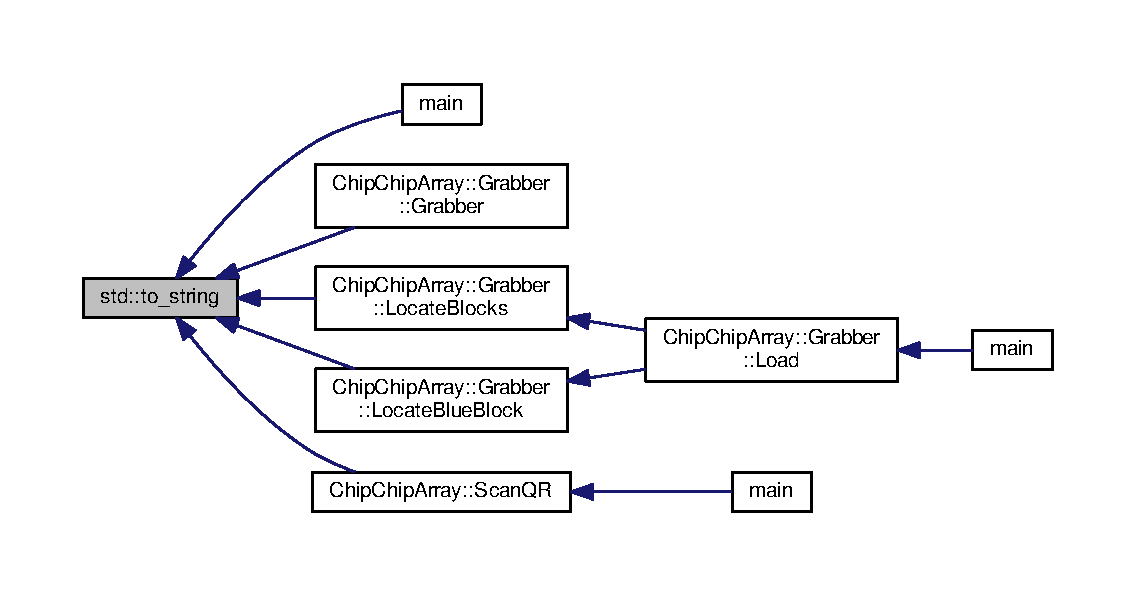
\includegraphics[width=350pt]{namespacestd_aa5ddf582a1c96ffe258c997be9a294a3_icgraph}
\end{center}
\end{figure}


\hypertarget{namespacestd_a6a0c3c323562edbd2f57da3d2bb74326}{\index{std@{std}!to\+\_\+string@{to\+\_\+string}}
\index{to\+\_\+string@{to\+\_\+string}!std@{std}}
\subsubsection[{to\+\_\+string}]{\setlength{\rightskip}{0pt plus 5cm}string std\+::to\+\_\+string (
\begin{DoxyParamCaption}
\item[{{\bf Color}}]{color}
\end{DoxyParamCaption}
)}}\label{namespacestd_a6a0c3c323562edbd2f57da3d2bb74326}
Converts a Color to a string. 

Definition at line 96 of file definitions.\+hpp.

\hypertarget{namespacestd_adb24d6df94a83c325573f7710df84953}{\index{std@{std}!to\+\_\+string@{to\+\_\+string}}
\index{to\+\_\+string@{to\+\_\+string}!std@{std}}
\subsubsection[{to\+\_\+string}]{\setlength{\rightskip}{0pt plus 5cm}string std\+::to\+\_\+string (
\begin{DoxyParamCaption}
\item[{{\bf Log\+Mode}}]{mode}
\end{DoxyParamCaption}
)}}\label{namespacestd_adb24d6df94a83c325573f7710df84953}
Converts a Log\+Mode to a string. 

Definition at line 123 of file definitions.\+hpp.

\hypertarget{namespacestd_a7fb649b1361ca7d95cc74045c0dadcdd}{\index{std@{std}!to\+\_\+string@{to\+\_\+string}}
\index{to\+\_\+string@{to\+\_\+string}!std@{std}}
\subsubsection[{to\+\_\+string}]{\setlength{\rightskip}{0pt plus 5cm}string std\+::to\+\_\+string (
\begin{DoxyParamCaption}
\item[{{\bf Result}}]{res}
\end{DoxyParamCaption}
)}}\label{namespacestd_a7fb649b1361ca7d95cc74045c0dadcdd}
Converts a Result to a string. 

Definition at line 131 of file definitions.\+hpp.

\hypertarget{namespacestd_aae21fd95009e4cc9fa25e1ad3830980b}{\index{std@{std}!to\+\_\+string@{to\+\_\+string}}
\index{to\+\_\+string@{to\+\_\+string}!std@{std}}
\subsubsection[{to\+\_\+string}]{\setlength{\rightskip}{0pt plus 5cm}string std\+::to\+\_\+string (
\begin{DoxyParamCaption}
\item[{{\bf Side}}]{side}
\end{DoxyParamCaption}
)}}\label{namespacestd_aae21fd95009e4cc9fa25e1ad3830980b}
Converts a Side to a string. 

Definition at line 158 of file definitions.\+hpp.

\hypertarget{namespacestd_a6bfcd2c3377165652c64085d7acb5c64}{\index{std@{std}!to\+\_\+string@{to\+\_\+string}}
\index{to\+\_\+string@{to\+\_\+string}!std@{std}}
\subsubsection[{to\+\_\+string}]{\setlength{\rightskip}{0pt plus 5cm}string std\+::to\+\_\+string (
\begin{DoxyParamCaption}
\item[{{\bf Size}}]{size}
\end{DoxyParamCaption}
)}}\label{namespacestd_a6bfcd2c3377165652c64085d7acb5c64}
Converts a Size to a string. 

Definition at line 166 of file definitions.\+hpp.

\hypertarget{namespacestd_ac50951e195256b4c2311f90189f64ba8}{\index{std@{std}!to\+\_\+string@{to\+\_\+string}}
\index{to\+\_\+string@{to\+\_\+string}!std@{std}}
\subsubsection[{to\+\_\+string}]{\setlength{\rightskip}{0pt plus 5cm}string std\+::to\+\_\+string (
\begin{DoxyParamCaption}
\item[{{\bf Zone}}]{zone}
\end{DoxyParamCaption}
)}}\label{namespacestd_ac50951e195256b4c2311f90189f64ba8}
Converts a Zone to a string. 

Definition at line 174 of file definitions.\+hpp.


\chapter{Class Documentation}
\hypertarget{classAdafruit__PWMServoDriver}{\section{Adafruit\+\_\+\+P\+W\+M\+Servo\+Driver Class Reference}
\label{classAdafruit__PWMServoDriver}\index{Adafruit\+\_\+\+P\+W\+M\+Servo\+Driver@{Adafruit\+\_\+\+P\+W\+M\+Servo\+Driver}}
}


{\ttfamily \#include $<$Adafruit\+\_\+\+P\+W\+M\+Servo\+Driver.\+h$>$}

\subsection*{Public Member Functions}
\begin{DoxyCompactItemize}
\item 
\hyperlink{classAdafruit__PWMServoDriver_a6a949db60836febbc61adef4cc5429ed}{Adafruit\+\_\+\+P\+W\+M\+Servo\+Driver} (\hyperlink{Servo__Position__Shell_8h_ab077fa1127453be2bd9d4c3c8a768fa7}{uint8\+\_\+t} addr=0x41)
\item 
void \hyperlink{classAdafruit__PWMServoDriver_aef401eaad3c34222ac916eb7bd936bc2}{begin} (void)
\item 
void \hyperlink{classAdafruit__PWMServoDriver_ac976f52233a75a4bd0eb6f2ce9b82b7f}{reset} (void)
\item 
void \hyperlink{classAdafruit__PWMServoDriver_a0ef6f1e3c81aebbd1d1da1bb12f3ed5c}{set\+P\+W\+M\+Freq} (float freq)
\item 
void \hyperlink{classAdafruit__PWMServoDriver_a724a7fc39c6fba34478ecc0eea038bd3}{set\+P\+W\+M} (\hyperlink{Servo__Position__Shell_8h_ab077fa1127453be2bd9d4c3c8a768fa7}{uint8\+\_\+t} num, \hyperlink{Adafruit__PWMServoDriver_8h_a395b3b2bf5cb4674ab41b6bda68c15bb}{uint16\+\_\+t} on, \hyperlink{Adafruit__PWMServoDriver_8h_a395b3b2bf5cb4674ab41b6bda68c15bb}{uint16\+\_\+t} off)
\item 
void \hyperlink{classAdafruit__PWMServoDriver_a1246cd50849fe0f068cc5d474e06ae96}{set\+Pin} (\hyperlink{Servo__Position__Shell_8h_ab077fa1127453be2bd9d4c3c8a768fa7}{uint8\+\_\+t} num, \hyperlink{Adafruit__PWMServoDriver_8h_a395b3b2bf5cb4674ab41b6bda68c15bb}{uint16\+\_\+t} val, bool invert=false)
\end{DoxyCompactItemize}


\subsection{Detailed Description}


Definition at line 65 of file Adafruit\+\_\+\+P\+W\+M\+Servo\+Driver.\+h.



\subsection{Constructor \& Destructor Documentation}
\hypertarget{classAdafruit__PWMServoDriver_a6a949db60836febbc61adef4cc5429ed}{\index{Adafruit\+\_\+\+P\+W\+M\+Servo\+Driver@{Adafruit\+\_\+\+P\+W\+M\+Servo\+Driver}!Adafruit\+\_\+\+P\+W\+M\+Servo\+Driver@{Adafruit\+\_\+\+P\+W\+M\+Servo\+Driver}}
\index{Adafruit\+\_\+\+P\+W\+M\+Servo\+Driver@{Adafruit\+\_\+\+P\+W\+M\+Servo\+Driver}!Adafruit\+\_\+\+P\+W\+M\+Servo\+Driver@{Adafruit\+\_\+\+P\+W\+M\+Servo\+Driver}}
\subsubsection[{Adafruit\+\_\+\+P\+W\+M\+Servo\+Driver}]{\setlength{\rightskip}{0pt plus 5cm}Adafruit\+\_\+\+P\+W\+M\+Servo\+Driver\+::\+Adafruit\+\_\+\+P\+W\+M\+Servo\+Driver (
\begin{DoxyParamCaption}
\item[{{\bf uint8\+\_\+t}}]{addr = {\ttfamily 0x41}}
\end{DoxyParamCaption}
)}}\label{classAdafruit__PWMServoDriver_a6a949db60836febbc61adef4cc5429ed}


Definition at line 29 of file Adafruit\+\_\+\+P\+W\+M\+Servo\+Driver.\+cpp.



\subsection{Member Function Documentation}
\hypertarget{classAdafruit__PWMServoDriver_aef401eaad3c34222ac916eb7bd936bc2}{\index{Adafruit\+\_\+\+P\+W\+M\+Servo\+Driver@{Adafruit\+\_\+\+P\+W\+M\+Servo\+Driver}!begin@{begin}}
\index{begin@{begin}!Adafruit\+\_\+\+P\+W\+M\+Servo\+Driver@{Adafruit\+\_\+\+P\+W\+M\+Servo\+Driver}}
\subsubsection[{begin}]{\setlength{\rightskip}{0pt plus 5cm}void Adafruit\+\_\+\+P\+W\+M\+Servo\+Driver\+::begin (
\begin{DoxyParamCaption}
\item[{void}]{}
\end{DoxyParamCaption}
)}}\label{classAdafruit__PWMServoDriver_aef401eaad3c34222ac916eb7bd936bc2}


Definition at line 34 of file Adafruit\+\_\+\+P\+W\+M\+Servo\+Driver.\+cpp.



Here is the call graph for this function\+:




Here is the caller graph for this function\+:


\hypertarget{classAdafruit__PWMServoDriver_ac976f52233a75a4bd0eb6f2ce9b82b7f}{\index{Adafruit\+\_\+\+P\+W\+M\+Servo\+Driver@{Adafruit\+\_\+\+P\+W\+M\+Servo\+Driver}!reset@{reset}}
\index{reset@{reset}!Adafruit\+\_\+\+P\+W\+M\+Servo\+Driver@{Adafruit\+\_\+\+P\+W\+M\+Servo\+Driver}}
\subsubsection[{reset}]{\setlength{\rightskip}{0pt plus 5cm}void Adafruit\+\_\+\+P\+W\+M\+Servo\+Driver\+::reset (
\begin{DoxyParamCaption}
\item[{void}]{}
\end{DoxyParamCaption}
)}}\label{classAdafruit__PWMServoDriver_ac976f52233a75a4bd0eb6f2ce9b82b7f}


Definition at line 42 of file Adafruit\+\_\+\+P\+W\+M\+Servo\+Driver.\+cpp.



Here is the caller graph for this function\+:


\hypertarget{classAdafruit__PWMServoDriver_a1246cd50849fe0f068cc5d474e06ae96}{\index{Adafruit\+\_\+\+P\+W\+M\+Servo\+Driver@{Adafruit\+\_\+\+P\+W\+M\+Servo\+Driver}!set\+Pin@{set\+Pin}}
\index{set\+Pin@{set\+Pin}!Adafruit\+\_\+\+P\+W\+M\+Servo\+Driver@{Adafruit\+\_\+\+P\+W\+M\+Servo\+Driver}}
\subsubsection[{set\+Pin}]{\setlength{\rightskip}{0pt plus 5cm}void Adafruit\+\_\+\+P\+W\+M\+Servo\+Driver\+::set\+Pin (
\begin{DoxyParamCaption}
\item[{{\bf uint8\+\_\+t}}]{num, }
\item[{{\bf uint16\+\_\+t}}]{val, }
\item[{bool}]{invert = {\ttfamily false}}
\end{DoxyParamCaption}
)}}\label{classAdafruit__PWMServoDriver_a1246cd50849fe0f068cc5d474e06ae96}


Definition at line 108 of file Adafruit\+\_\+\+P\+W\+M\+Servo\+Driver.\+cpp.



Here is the call graph for this function\+:


\hypertarget{classAdafruit__PWMServoDriver_a724a7fc39c6fba34478ecc0eea038bd3}{\index{Adafruit\+\_\+\+P\+W\+M\+Servo\+Driver@{Adafruit\+\_\+\+P\+W\+M\+Servo\+Driver}!set\+P\+W\+M@{set\+P\+W\+M}}
\index{set\+P\+W\+M@{set\+P\+W\+M}!Adafruit\+\_\+\+P\+W\+M\+Servo\+Driver@{Adafruit\+\_\+\+P\+W\+M\+Servo\+Driver}}
\subsubsection[{set\+P\+W\+M}]{\setlength{\rightskip}{0pt plus 5cm}void Adafruit\+\_\+\+P\+W\+M\+Servo\+Driver\+::set\+P\+W\+M (
\begin{DoxyParamCaption}
\item[{{\bf uint8\+\_\+t}}]{num, }
\item[{{\bf uint16\+\_\+t}}]{on, }
\item[{{\bf uint16\+\_\+t}}]{off}
\end{DoxyParamCaption}
)}}\label{classAdafruit__PWMServoDriver_a724a7fc39c6fba34478ecc0eea038bd3}


Definition at line 73 of file Adafruit\+\_\+\+P\+W\+M\+Servo\+Driver.\+cpp.



Here is the caller graph for this function\+:


\hypertarget{classAdafruit__PWMServoDriver_a0ef6f1e3c81aebbd1d1da1bb12f3ed5c}{\index{Adafruit\+\_\+\+P\+W\+M\+Servo\+Driver@{Adafruit\+\_\+\+P\+W\+M\+Servo\+Driver}!set\+P\+W\+M\+Freq@{set\+P\+W\+M\+Freq}}
\index{set\+P\+W\+M\+Freq@{set\+P\+W\+M\+Freq}!Adafruit\+\_\+\+P\+W\+M\+Servo\+Driver@{Adafruit\+\_\+\+P\+W\+M\+Servo\+Driver}}
\subsubsection[{set\+P\+W\+M\+Freq}]{\setlength{\rightskip}{0pt plus 5cm}void Adafruit\+\_\+\+P\+W\+M\+Servo\+Driver\+::set\+P\+W\+M\+Freq (
\begin{DoxyParamCaption}
\item[{float}]{freq}
\end{DoxyParamCaption}
)}}\label{classAdafruit__PWMServoDriver_a0ef6f1e3c81aebbd1d1da1bb12f3ed5c}


Definition at line 46 of file Adafruit\+\_\+\+P\+W\+M\+Servo\+Driver.\+cpp.



Here is the caller graph for this function\+:




The documentation for this class was generated from the following files\+:\begin{DoxyCompactItemize}
\item 
src/\hyperlink{Adafruit__PWMServoDriver_8h}{Adafruit\+\_\+\+P\+W\+M\+Servo\+Driver.\+h}\item 
src/\hyperlink{Adafruit__PWMServoDriver_8cpp}{Adafruit\+\_\+\+P\+W\+M\+Servo\+Driver.\+cpp}\end{DoxyCompactItemize}

\hypertarget{classChipChipArray_1_1Block}{\section{Chip\+Chip\+Array\+:\+:Block Class Reference}
\label{classChipChipArray_1_1Block}\index{Chip\+Chip\+Array\+::\+Block@{Chip\+Chip\+Array\+::\+Block}}
}


{\ttfamily \#include $<$Block.\+hpp$>$}

\subsection*{Public Member Functions}
\begin{DoxyCompactItemize}
\item 
\hyperlink{classChipChipArray_1_1Block_a7eb2456e5c95c8a91844c9522eed0578}{Block} (cv\+::\+Rect rect, \hyperlink{definitions_8hpp_abc05a0f46084a3477cf5d5c939ff1436}{Color} \hyperlink{classChipChipArray_1_1Block_a262210a9a04028f3f2670c9ae38ef3d7}{color})
\end{DoxyCompactItemize}
\subsection*{Public Attributes}
\begin{DoxyCompactItemize}
\item 
\hyperlink{definitions_8hpp_a1134b580f8da4de94ca6b1de4d37975e}{uint32} \hyperlink{classChipChipArray_1_1Block_ab5f9a9c1cc11e949685f8ad3d52599b2}{area}
\item 
cv\+::\+Point \hyperlink{classChipChipArray_1_1Block_a78304b597a8d8a74a4d9b4bb561a7224}{bottom\+Left}
\item 
cv\+::\+Point \hyperlink{classChipChipArray_1_1Block_a82f831883d31e6d74be45b8851eefe96}{bottom\+Right}
\item 
\hyperlink{definitions_8hpp_a74df79fde3c518e55b29ce6360a9c76e}{sint16} \hyperlink{classChipChipArray_1_1Block_af3c4ecd0fd36763ac85c2dc0b57b8359}{d\+Bottom}
\item 
\hyperlink{definitions_8hpp_a74df79fde3c518e55b29ce6360a9c76e}{sint16} \hyperlink{classChipChipArray_1_1Block_aca89dc06d62feb9a6478a06976171b2b}{d\+Left}
\item 
\hyperlink{definitions_8hpp_a74df79fde3c518e55b29ce6360a9c76e}{sint16} \hyperlink{classChipChipArray_1_1Block_a6a4b0aa6aae7e41d836c8955e209c16e}{d\+Right}
\item 
\hyperlink{definitions_8hpp_a74df79fde3c518e55b29ce6360a9c76e}{sint16} \hyperlink{classChipChipArray_1_1Block_a4e792a05f677eafbeb9439a9e631c255}{d\+Top}
\item 
\hyperlink{definitions_8hpp_a74df79fde3c518e55b29ce6360a9c76e}{sint16} \hyperlink{classChipChipArray_1_1Block_a5b6e72665d0de840a123717e24ca5cf9}{d\+Top\+Bottom}
\item 
\hyperlink{definitions_8hpp_a74df79fde3c518e55b29ce6360a9c76e}{sint16} \hyperlink{classChipChipArray_1_1Block_a2d02c7b99ca656960fc9724587791999}{d\+Right\+Left}
\item 
\hyperlink{definitions_8hpp_a74df79fde3c518e55b29ce6360a9c76e}{sint16} \hyperlink{classChipChipArray_1_1Block_a42e2ca0775dc09b04049a2db1bc0bb4f}{offset}
\item 
\hyperlink{definitions_8hpp_a05f6b0ae8f6a6e135b0e290c25fe0e4e}{uint16} \hyperlink{classChipChipArray_1_1Block_aed94802c166c9b4553764eb637717a2a}{height}
\item 
cv\+::\+Point \hyperlink{classChipChipArray_1_1Block_aeecc05025c6c8e23ff6ca09a6fbd4b4b}{top\+Left}
\item 
cv\+::\+Point \hyperlink{classChipChipArray_1_1Block_aaa4ff82846e95a628800ebdfd3ceefb5}{top\+Right}
\item 
\hyperlink{definitions_8hpp_a05f6b0ae8f6a6e135b0e290c25fe0e4e}{uint16} \hyperlink{classChipChipArray_1_1Block_ac3f815e8aa9060c4ad20d4e1b2649e35}{width}
\item 
\hyperlink{definitions_8hpp_abc05a0f46084a3477cf5d5c939ff1436}{Color} \hyperlink{classChipChipArray_1_1Block_a262210a9a04028f3f2670c9ae38ef3d7}{color}
\item 
\hyperlink{definitions_8hpp_a9809446fd16a744b6df9808293f14153}{Size} \hyperlink{classChipChipArray_1_1Block_aebd356d7fcfe7ff11db8195e6d7f8e42}{size}
\end{DoxyCompactItemize}


\subsection{Detailed Description}
This class represents a block. It only works for blocks found with the \char`\"{}bounding\+Rect\char`\"{} algorithm (i.\+e., it doesn't work for blocks that are skewed on the image). 

Definition at line \hyperlink{Block_8hpp_source_l00020}{20} of file \hyperlink{Block_8hpp_source}{Block.\+hpp}.



\subsection{Constructor \& Destructor Documentation}
\hypertarget{classChipChipArray_1_1Block_a7eb2456e5c95c8a91844c9522eed0578}{\index{Chip\+Chip\+Array\+::\+Block@{Chip\+Chip\+Array\+::\+Block}!Block@{Block}}
\index{Block@{Block}!Chip\+Chip\+Array\+::\+Block@{Chip\+Chip\+Array\+::\+Block}}
\subsubsection[{Block}]{\setlength{\rightskip}{0pt plus 5cm}Chip\+Chip\+Array\+::\+Block\+::\+Block (
\begin{DoxyParamCaption}
\item[{cv\+::\+Rect}]{rect, }
\item[{{\bf Color}}]{color}
\end{DoxyParamCaption}
)}}\label{classChipChipArray_1_1Block_a7eb2456e5c95c8a91844c9522eed0578}
Creates a new \hyperlink{classChipChipArray_1_1Block}{Block} using the Points in the cv\+::\+Rect and the color. Also determines the size based on the area of the \hyperlink{classChipChipArray_1_1Block}{Block}. 

Definition at line \hyperlink{Block_8hpp_source_l00139}{139} of file \hyperlink{Block_8hpp_source}{Block.\+hpp}.


\begin{DoxyCode}
00139                                          \{
00140         \textcolor{comment}{// basic geometric properties}
00141         \hyperlink{classChipChipArray_1_1Block_ab5f9a9c1cc11e949685f8ad3d52599b2}{area} = rect.area();
00142         \hyperlink{classChipChipArray_1_1Block_aed94802c166c9b4553764eb637717a2a}{height} = rect.height;
00143         \hyperlink{classChipChipArray_1_1Block_ac3f815e8aa9060c4ad20d4e1b2649e35}{width} = rect.width;
00144 
00145         \textcolor{comment}{// assigning corners}
00146         \hyperlink{classChipChipArray_1_1Block_aeecc05025c6c8e23ff6ca09a6fbd4b4b}{topLeft} = rect.tl();
00147         \hyperlink{classChipChipArray_1_1Block_a82f831883d31e6d74be45b8851eefe96}{bottomRight} = rect.br();
00148         \hyperlink{classChipChipArray_1_1Block_aaa4ff82846e95a628800ebdfd3ceefb5}{topRight} = cv::Point(\hyperlink{classChipChipArray_1_1Block_aeecc05025c6c8e23ff6ca09a6fbd4b4b}{topLeft}.x + \hyperlink{classChipChipArray_1_1Block_ac3f815e8aa9060c4ad20d4e1b2649e35}{width}, \hyperlink{classChipChipArray_1_1Block_aeecc05025c6c8e23ff6ca09a6fbd4b4b}{topLeft}.y);
00149         \hyperlink{classChipChipArray_1_1Block_a78304b597a8d8a74a4d9b4bb561a7224}{bottomLeft} = cv::Point(\hyperlink{classChipChipArray_1_1Block_aeecc05025c6c8e23ff6ca09a6fbd4b4b}{topLeft}.x, \hyperlink{classChipChipArray_1_1Block_aeecc05025c6c8e23ff6ca09a6fbd4b4b}{topLeft}.y + 
      \hyperlink{classChipChipArray_1_1Block_aed94802c166c9b4553764eb637717a2a}{height});
00150         \hyperlink{classChipChipArray_1_1Block_a42e2ca0775dc09b04049a2db1bc0bb4f}{offset} = (\hyperlink{definitions_8hpp_a74df79fde3c518e55b29ce6360a9c76e}{sint16})(\hyperlink{classChipChipArray_1_1Block_aeecc05025c6c8e23ff6ca09a6fbd4b4b}{topLeft}.x + \hyperlink{classChipChipArray_1_1Block_ac3f815e8aa9060c4ad20d4e1b2649e35}{width} / 2) - IMG\_WIDTH / 2;
00151 
00152         \textcolor{comment}{// calculating offsets (opencv low coordinates start top left)}
00153         \hyperlink{classChipChipArray_1_1Block_aca89dc06d62feb9a6478a06976171b2b}{dLeft} = \hyperlink{classChipChipArray_1_1Block_aeecc05025c6c8e23ff6ca09a6fbd4b4b}{topLeft}.x;
00154         \hyperlink{classChipChipArray_1_1Block_a6a4b0aa6aae7e41d836c8955e209c16e}{dRight} = IMG\_WIDTH - \hyperlink{classChipChipArray_1_1Block_aaa4ff82846e95a628800ebdfd3ceefb5}{topRight}.x;
00155         \hyperlink{classChipChipArray_1_1Block_a4e792a05f677eafbeb9439a9e631c255}{dTop} = \hyperlink{classChipChipArray_1_1Block_aeecc05025c6c8e23ff6ca09a6fbd4b4b}{topLeft}.y;
00156         \hyperlink{classChipChipArray_1_1Block_af3c4ecd0fd36763ac85c2dc0b57b8359}{dBottom} = IMG\_HEIGHT - \hyperlink{classChipChipArray_1_1Block_a82f831883d31e6d74be45b8851eefe96}{bottomRight}.y;
00157         \hyperlink{classChipChipArray_1_1Block_a5b6e72665d0de840a123717e24ca5cf9}{dTopBottom} = \hyperlink{classChipChipArray_1_1Block_a4e792a05f677eafbeb9439a9e631c255}{dTop} - \hyperlink{classChipChipArray_1_1Block_af3c4ecd0fd36763ac85c2dc0b57b8359}{dBottom};
00158         \hyperlink{classChipChipArray_1_1Block_a2d02c7b99ca656960fc9724587791999}{dRightLeft} = \hyperlink{classChipChipArray_1_1Block_a6a4b0aa6aae7e41d836c8955e209c16e}{dRight} - \hyperlink{classChipChipArray_1_1Block_aca89dc06d62feb9a6478a06976171b2b}{dLeft};
00159 
00160         \textcolor{comment}{// set color and size}
00161         this->\hyperlink{classChipChipArray_1_1Block_a262210a9a04028f3f2670c9ae38ef3d7}{color} = \hyperlink{classChipChipArray_1_1Block_a262210a9a04028f3f2670c9ae38ef3d7}{color};
00162         \hyperlink{classChipChipArray_1_1Block_aebd356d7fcfe7ff11db8195e6d7f8e42}{size} = \hyperlink{classChipChipArray_1_1Block_ab5f9a9c1cc11e949685f8ad3d52599b2}{area} > MIN\_WHOLE\_BLOCK\_SIZE ? \hyperlink{definitions_8hpp_a9809446fd16a744b6df9808293f14153a8394f0347c184cf156ac5924dccb773b}{Size::Long} : 
      \hyperlink{definitions_8hpp_a9809446fd16a744b6df9808293f14153a30bb747c98bccdd11b3f89e644c4d0ad}{Size::Short};
00163     \}
\end{DoxyCode}


\subsection{Member Data Documentation}
\hypertarget{classChipChipArray_1_1Block_ab5f9a9c1cc11e949685f8ad3d52599b2}{\index{Chip\+Chip\+Array\+::\+Block@{Chip\+Chip\+Array\+::\+Block}!area@{area}}
\index{area@{area}!Chip\+Chip\+Array\+::\+Block@{Chip\+Chip\+Array\+::\+Block}}
\subsubsection[{area}]{\setlength{\rightskip}{0pt plus 5cm}{\bf uint32} Chip\+Chip\+Array\+::\+Block\+::area}}\label{classChipChipArray_1_1Block_ab5f9a9c1cc11e949685f8ad3d52599b2}
The area of the block in pixels 

Definition at line \hyperlink{Block_8hpp_source_l00025}{25} of file \hyperlink{Block_8hpp_source}{Block.\+hpp}.

\hypertarget{classChipChipArray_1_1Block_a78304b597a8d8a74a4d9b4bb561a7224}{\index{Chip\+Chip\+Array\+::\+Block@{Chip\+Chip\+Array\+::\+Block}!bottom\+Left@{bottom\+Left}}
\index{bottom\+Left@{bottom\+Left}!Chip\+Chip\+Array\+::\+Block@{Chip\+Chip\+Array\+::\+Block}}
\subsubsection[{bottom\+Left}]{\setlength{\rightskip}{0pt plus 5cm}cv\+::\+Point Chip\+Chip\+Array\+::\+Block\+::bottom\+Left}}\label{classChipChipArray_1_1Block_a78304b597a8d8a74a4d9b4bb561a7224}
Point of the block's bottom-\/left corner 

Definition at line \hyperlink{Block_8hpp_source_l00030}{30} of file \hyperlink{Block_8hpp_source}{Block.\+hpp}.

\hypertarget{classChipChipArray_1_1Block_a82f831883d31e6d74be45b8851eefe96}{\index{Chip\+Chip\+Array\+::\+Block@{Chip\+Chip\+Array\+::\+Block}!bottom\+Right@{bottom\+Right}}
\index{bottom\+Right@{bottom\+Right}!Chip\+Chip\+Array\+::\+Block@{Chip\+Chip\+Array\+::\+Block}}
\subsubsection[{bottom\+Right}]{\setlength{\rightskip}{0pt plus 5cm}cv\+::\+Point Chip\+Chip\+Array\+::\+Block\+::bottom\+Right}}\label{classChipChipArray_1_1Block_a82f831883d31e6d74be45b8851eefe96}
Point of the block's bottom-\/right corner 

Definition at line \hyperlink{Block_8hpp_source_l00035}{35} of file \hyperlink{Block_8hpp_source}{Block.\+hpp}.

\hypertarget{classChipChipArray_1_1Block_a262210a9a04028f3f2670c9ae38ef3d7}{\index{Chip\+Chip\+Array\+::\+Block@{Chip\+Chip\+Array\+::\+Block}!color@{color}}
\index{color@{color}!Chip\+Chip\+Array\+::\+Block@{Chip\+Chip\+Array\+::\+Block}}
\subsubsection[{color}]{\setlength{\rightskip}{0pt plus 5cm}{\bf Color} Chip\+Chip\+Array\+::\+Block\+::color}}\label{classChipChipArray_1_1Block_a262210a9a04028f3f2670c9ae38ef3d7}
The detected color of the block 

Definition at line \hyperlink{Block_8hpp_source_l00107}{107} of file \hyperlink{Block_8hpp_source}{Block.\+hpp}.

\hypertarget{classChipChipArray_1_1Block_af3c4ecd0fd36763ac85c2dc0b57b8359}{\index{Chip\+Chip\+Array\+::\+Block@{Chip\+Chip\+Array\+::\+Block}!d\+Bottom@{d\+Bottom}}
\index{d\+Bottom@{d\+Bottom}!Chip\+Chip\+Array\+::\+Block@{Chip\+Chip\+Array\+::\+Block}}
\subsubsection[{d\+Bottom}]{\setlength{\rightskip}{0pt plus 5cm}{\bf sint16} Chip\+Chip\+Array\+::\+Block\+::d\+Bottom}}\label{classChipChipArray_1_1Block_af3c4ecd0fd36763ac85c2dc0b57b8359}
Number of pixels from the block's bottom edge to the bottom edge of the image frame. 

Definition at line \hyperlink{Block_8hpp_source_l00041}{41} of file \hyperlink{Block_8hpp_source}{Block.\+hpp}.

\hypertarget{classChipChipArray_1_1Block_aca89dc06d62feb9a6478a06976171b2b}{\index{Chip\+Chip\+Array\+::\+Block@{Chip\+Chip\+Array\+::\+Block}!d\+Left@{d\+Left}}
\index{d\+Left@{d\+Left}!Chip\+Chip\+Array\+::\+Block@{Chip\+Chip\+Array\+::\+Block}}
\subsubsection[{d\+Left}]{\setlength{\rightskip}{0pt plus 5cm}{\bf sint16} Chip\+Chip\+Array\+::\+Block\+::d\+Left}}\label{classChipChipArray_1_1Block_aca89dc06d62feb9a6478a06976171b2b}
Number of pixels from the block's left edge to the left edge of the image frame. 

Definition at line \hyperlink{Block_8hpp_source_l00047}{47} of file \hyperlink{Block_8hpp_source}{Block.\+hpp}.

\hypertarget{classChipChipArray_1_1Block_a6a4b0aa6aae7e41d836c8955e209c16e}{\index{Chip\+Chip\+Array\+::\+Block@{Chip\+Chip\+Array\+::\+Block}!d\+Right@{d\+Right}}
\index{d\+Right@{d\+Right}!Chip\+Chip\+Array\+::\+Block@{Chip\+Chip\+Array\+::\+Block}}
\subsubsection[{d\+Right}]{\setlength{\rightskip}{0pt plus 5cm}{\bf sint16} Chip\+Chip\+Array\+::\+Block\+::d\+Right}}\label{classChipChipArray_1_1Block_a6a4b0aa6aae7e41d836c8955e209c16e}
Number of pixels from the block's right edge to the right edge of the image frame. 

Definition at line \hyperlink{Block_8hpp_source_l00053}{53} of file \hyperlink{Block_8hpp_source}{Block.\+hpp}.

\hypertarget{classChipChipArray_1_1Block_a2d02c7b99ca656960fc9724587791999}{\index{Chip\+Chip\+Array\+::\+Block@{Chip\+Chip\+Array\+::\+Block}!d\+Right\+Left@{d\+Right\+Left}}
\index{d\+Right\+Left@{d\+Right\+Left}!Chip\+Chip\+Array\+::\+Block@{Chip\+Chip\+Array\+::\+Block}}
\subsubsection[{d\+Right\+Left}]{\setlength{\rightskip}{0pt plus 5cm}{\bf sint16} Chip\+Chip\+Array\+::\+Block\+::d\+Right\+Left}}\label{classChipChipArray_1_1Block_a2d02c7b99ca656960fc9724587791999}
The difference between d\+Right and d\+Left. It indicates the relative vertical positioning of the block regardless of the block's area. A positive value indicates the block is off-\/center towards the left. 

Definition at line \hyperlink{Block_8hpp_source_l00075}{75} of file \hyperlink{Block_8hpp_source}{Block.\+hpp}.

\hypertarget{classChipChipArray_1_1Block_a4e792a05f677eafbeb9439a9e631c255}{\index{Chip\+Chip\+Array\+::\+Block@{Chip\+Chip\+Array\+::\+Block}!d\+Top@{d\+Top}}
\index{d\+Top@{d\+Top}!Chip\+Chip\+Array\+::\+Block@{Chip\+Chip\+Array\+::\+Block}}
\subsubsection[{d\+Top}]{\setlength{\rightskip}{0pt plus 5cm}{\bf sint16} Chip\+Chip\+Array\+::\+Block\+::d\+Top}}\label{classChipChipArray_1_1Block_a4e792a05f677eafbeb9439a9e631c255}
Number of pixels from the block's top edge to the top edge of the image frame. 

Definition at line \hyperlink{Block_8hpp_source_l00059}{59} of file \hyperlink{Block_8hpp_source}{Block.\+hpp}.

\hypertarget{classChipChipArray_1_1Block_a5b6e72665d0de840a123717e24ca5cf9}{\index{Chip\+Chip\+Array\+::\+Block@{Chip\+Chip\+Array\+::\+Block}!d\+Top\+Bottom@{d\+Top\+Bottom}}
\index{d\+Top\+Bottom@{d\+Top\+Bottom}!Chip\+Chip\+Array\+::\+Block@{Chip\+Chip\+Array\+::\+Block}}
\subsubsection[{d\+Top\+Bottom}]{\setlength{\rightskip}{0pt plus 5cm}{\bf sint16} Chip\+Chip\+Array\+::\+Block\+::d\+Top\+Bottom}}\label{classChipChipArray_1_1Block_a5b6e72665d0de840a123717e24ca5cf9}
The difference between d\+Top and d\+Bottom. It indicates the relative vertical positioning of the block regardless of the block's area. A positive value indicates the block is off-\/center towards the bottom. 

Definition at line \hyperlink{Block_8hpp_source_l00067}{67} of file \hyperlink{Block_8hpp_source}{Block.\+hpp}.

\hypertarget{classChipChipArray_1_1Block_aed94802c166c9b4553764eb637717a2a}{\index{Chip\+Chip\+Array\+::\+Block@{Chip\+Chip\+Array\+::\+Block}!height@{height}}
\index{height@{height}!Chip\+Chip\+Array\+::\+Block@{Chip\+Chip\+Array\+::\+Block}}
\subsubsection[{height}]{\setlength{\rightskip}{0pt plus 5cm}{\bf uint16} Chip\+Chip\+Array\+::\+Block\+::height}}\label{classChipChipArray_1_1Block_aed94802c166c9b4553764eb637717a2a}
The height of the block in pixels 

Definition at line \hyperlink{Block_8hpp_source_l00087}{87} of file \hyperlink{Block_8hpp_source}{Block.\+hpp}.

\hypertarget{classChipChipArray_1_1Block_a42e2ca0775dc09b04049a2db1bc0bb4f}{\index{Chip\+Chip\+Array\+::\+Block@{Chip\+Chip\+Array\+::\+Block}!offset@{offset}}
\index{offset@{offset}!Chip\+Chip\+Array\+::\+Block@{Chip\+Chip\+Array\+::\+Block}}
\subsubsection[{offset}]{\setlength{\rightskip}{0pt plus 5cm}{\bf sint16} Chip\+Chip\+Array\+::\+Block\+::offset}}\label{classChipChipArray_1_1Block_a42e2ca0775dc09b04049a2db1bc0bb4f}
The difference in pixels between the vertical center of the image and the vertical center of the block. Assumes image is 1280 pixels wide (like the Raspicam images). 

Definition at line \hyperlink{Block_8hpp_source_l00082}{82} of file \hyperlink{Block_8hpp_source}{Block.\+hpp}.

\hypertarget{classChipChipArray_1_1Block_aebd356d7fcfe7ff11db8195e6d7f8e42}{\index{Chip\+Chip\+Array\+::\+Block@{Chip\+Chip\+Array\+::\+Block}!size@{size}}
\index{size@{size}!Chip\+Chip\+Array\+::\+Block@{Chip\+Chip\+Array\+::\+Block}}
\subsubsection[{size}]{\setlength{\rightskip}{0pt plus 5cm}{\bf Size} Chip\+Chip\+Array\+::\+Block\+::size}}\label{classChipChipArray_1_1Block_aebd356d7fcfe7ff11db8195e6d7f8e42}
The size of the block (half or whole) 

Definition at line \hyperlink{Block_8hpp_source_l00112}{112} of file \hyperlink{Block_8hpp_source}{Block.\+hpp}.

\hypertarget{classChipChipArray_1_1Block_aeecc05025c6c8e23ff6ca09a6fbd4b4b}{\index{Chip\+Chip\+Array\+::\+Block@{Chip\+Chip\+Array\+::\+Block}!top\+Left@{top\+Left}}
\index{top\+Left@{top\+Left}!Chip\+Chip\+Array\+::\+Block@{Chip\+Chip\+Array\+::\+Block}}
\subsubsection[{top\+Left}]{\setlength{\rightskip}{0pt plus 5cm}cv\+::\+Point Chip\+Chip\+Array\+::\+Block\+::top\+Left}}\label{classChipChipArray_1_1Block_aeecc05025c6c8e23ff6ca09a6fbd4b4b}
Point of the block's top-\/left corner 

Definition at line \hyperlink{Block_8hpp_source_l00092}{92} of file \hyperlink{Block_8hpp_source}{Block.\+hpp}.

\hypertarget{classChipChipArray_1_1Block_aaa4ff82846e95a628800ebdfd3ceefb5}{\index{Chip\+Chip\+Array\+::\+Block@{Chip\+Chip\+Array\+::\+Block}!top\+Right@{top\+Right}}
\index{top\+Right@{top\+Right}!Chip\+Chip\+Array\+::\+Block@{Chip\+Chip\+Array\+::\+Block}}
\subsubsection[{top\+Right}]{\setlength{\rightskip}{0pt plus 5cm}cv\+::\+Point Chip\+Chip\+Array\+::\+Block\+::top\+Right}}\label{classChipChipArray_1_1Block_aaa4ff82846e95a628800ebdfd3ceefb5}
Point of the block's top-\/right corner 

Definition at line \hyperlink{Block_8hpp_source_l00097}{97} of file \hyperlink{Block_8hpp_source}{Block.\+hpp}.

\hypertarget{classChipChipArray_1_1Block_ac3f815e8aa9060c4ad20d4e1b2649e35}{\index{Chip\+Chip\+Array\+::\+Block@{Chip\+Chip\+Array\+::\+Block}!width@{width}}
\index{width@{width}!Chip\+Chip\+Array\+::\+Block@{Chip\+Chip\+Array\+::\+Block}}
\subsubsection[{width}]{\setlength{\rightskip}{0pt plus 5cm}{\bf uint16} Chip\+Chip\+Array\+::\+Block\+::width}}\label{classChipChipArray_1_1Block_ac3f815e8aa9060c4ad20d4e1b2649e35}
The width of the block in pixels 

Definition at line \hyperlink{Block_8hpp_source_l00102}{102} of file \hyperlink{Block_8hpp_source}{Block.\+hpp}.



The documentation for this class was generated from the following file\+:\begin{DoxyCompactItemize}
\item 
src/\hyperlink{Block_8hpp}{Block.\+hpp}\end{DoxyCompactItemize}

\hypertarget{classChipChipArray_1_1Grabber}{\section{Chip\+Chip\+Array\+:\+:Grabber Class Reference}
\label{classChipChipArray_1_1Grabber}\index{Chip\+Chip\+Array\+::\+Grabber@{Chip\+Chip\+Array\+::\+Grabber}}
}


{\ttfamily \#include $<$Grabber.\+hpp$>$}



Collaboration diagram for Chip\+Chip\+Array\+:\+:Grabber\+:
\nopagebreak
\begin{figure}[H]
\begin{center}
\leavevmode
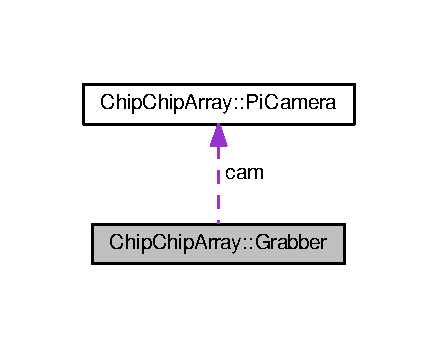
\includegraphics[width=210pt]{classChipChipArray_1_1Grabber__coll__graph}
\end{center}
\end{figure}
\subsection*{Public Member Functions}
\begin{DoxyCompactItemize}
\item 
\hyperlink{classChipChipArray_1_1Grabber_a7333f40c135fbe92d59651f75032b4e7}{Grabber} (\hyperlink{definitions_8hpp_adbd1e7a33d3e1751c7b2aa2562d0ecb9}{Zone} \hyperlink{classChipChipArray_1_1Grabber_ab57efe6e0b6f369b19528285a278d967}{zone}, \hyperlink{definitions_8hpp_a03325a8a9d4f105db5e37dd587128142}{Side} \hyperlink{classChipChipArray_1_1Grabber_a8afbaefae7c767c862fd1bf13968539b}{side})
\item 
void \hyperlink{classChipChipArray_1_1Grabber_aacf089ceb4aa5b263c2cc702fb3daf74}{Close} ()
\item 
\hyperlink{definitions_8hpp_ab84ebabb02540c4a7ec341a213abf1dc}{Result} \hyperlink{classChipChipArray_1_1Grabber_a56639f8f9ba9468bce4b6d69ceb2eb54}{Load} ()
\end{DoxyCompactItemize}
\subsection*{Protected Member Functions}
\begin{DoxyCompactItemize}
\item 
void \hyperlink{classChipChipArray_1_1Grabber_a44e5aeb908634f68de356ad8df3c4bf1}{Deposit} (\hyperlink{definitions_8hpp_abc05a0f46084a3477cf5d5c939ff1436}{Color} color=\hyperlink{definitions_8hpp_abc05a0f46084a3477cf5d5c939ff1436a9594eec95be70e7b1710f730fdda33d9}{Color\+::\+Blue})
\item 
void \hyperlink{classChipChipArray_1_1Grabber_abecb4047b4f7d5a7e691b7fb581b5a39}{Extend} ()
\item 
\hyperlink{classChipChipArray_1_1Block}{Block} \hyperlink{classChipChipArray_1_1Grabber_af49248c957a1695dcde79c0f5f8df99b}{Locate\+Blocks} (\hyperlink{definitions_8hpp_abc05a0f46084a3477cf5d5c939ff1436}{Color} color=\hyperlink{definitions_8hpp_abc05a0f46084a3477cf5d5c939ff1436a1e700ac224a6d34c5b171bb6f462aa41}{Color\+::\+Perrywinkle})
\item 
\hyperlink{classChipChipArray_1_1Block}{Block} \hyperlink{classChipChipArray_1_1Grabber_ab9b0d6a64b2c94c0d0f810a5ebeef6ec}{Locate\+Blue\+Block} ()
\end{DoxyCompactItemize}
\subsection*{Protected Attributes}
\begin{DoxyCompactItemize}
\item 
\hyperlink{classChipChipArray_1_1PiCamera}{Pi\+Camera} \hyperlink{classChipChipArray_1_1Grabber_a726bcc2367a719cb84de92a981947622}{cam}
\item 
\hyperlink{definitions_8hpp_a03325a8a9d4f105db5e37dd587128142}{Side} \hyperlink{classChipChipArray_1_1Grabber_a8afbaefae7c767c862fd1bf13968539b}{side}
\item 
\hyperlink{definitions_8hpp_adbd1e7a33d3e1751c7b2aa2562d0ecb9}{Zone} \hyperlink{classChipChipArray_1_1Grabber_ab57efe6e0b6f369b19528285a278d967}{zone}
\end{DoxyCompactItemize}


\subsection{Detailed Description}
This class finds blocks, identifies them, and sorts them according to color, size, and zone. 

Definition at line \hyperlink{Grabber_8hpp_source_l00030}{30} of file \hyperlink{Grabber_8hpp_source}{Grabber.\+hpp}.



\subsection{Constructor \& Destructor Documentation}
\hypertarget{classChipChipArray_1_1Grabber_a7333f40c135fbe92d59651f75032b4e7}{\index{Chip\+Chip\+Array\+::\+Grabber@{Chip\+Chip\+Array\+::\+Grabber}!Grabber@{Grabber}}
\index{Grabber@{Grabber}!Chip\+Chip\+Array\+::\+Grabber@{Chip\+Chip\+Array\+::\+Grabber}}
\subsubsection[{Grabber}]{\setlength{\rightskip}{0pt plus 5cm}Chip\+Chip\+Array\+::\+Grabber\+::\+Grabber (
\begin{DoxyParamCaption}
\item[{{\bf Zone}}]{zone, }
\item[{{\bf Side}}]{side}
\end{DoxyParamCaption}
)}}\label{classChipChipArray_1_1Grabber_a7333f40c135fbe92d59651f75032b4e7}
Initializes the class according to the side and zone and extends the robotic arm into position.


\begin{DoxyParams}{Parameters}
{\em zone} & the zone (A, B, or C) for which to pick up blocks.\\
\hline
{\em side} & the side from which the robot is moving and the position of the blocks (right or left) in the view of the camera to pick up first \\
\hline
\end{DoxyParams}


Definition at line \hyperlink{Grabber_8hpp_source_l00143}{143} of file \hyperlink{Grabber_8hpp_source}{Grabber.\+hpp}.


\begin{DoxyCode}
00143                                          \{
00144         log.\hyperlink{classChipChipArray_1_1Log_a66575b6e94c6112e4cefa5736cb996e0}{Status}(\textcolor{stringliteral}{"Opening Grabber"});
00145         log.\hyperlink{classChipChipArray_1_1Log_a154a5f38d9c7a767693b242684a3d4d9}{Verbose}(\textcolor{stringliteral}{"Zone: "} + \hyperlink{namespacestd_aa5ddf582a1c96ffe258c997be9a294a3}{std::to\_string}(\hyperlink{classChipChipArray_1_1Grabber_ab57efe6e0b6f369b19528285a278d967}{zone}));
00146         log.\hyperlink{classChipChipArray_1_1Log_a154a5f38d9c7a767693b242684a3d4d9}{Verbose}(\textcolor{stringliteral}{"Side: "} + \hyperlink{namespacestd_aa5ddf582a1c96ffe258c997be9a294a3}{std::to\_string}(\hyperlink{classChipChipArray_1_1Grabber_a8afbaefae7c767c862fd1bf13968539b}{side}));
00147 
00148         this->\hyperlink{classChipChipArray_1_1Grabber_ab57efe6e0b6f369b19528285a278d967}{zone} = \hyperlink{classChipChipArray_1_1Grabber_ab57efe6e0b6f369b19528285a278d967}{zone};
00149         this->\hyperlink{classChipChipArray_1_1Grabber_a8afbaefae7c767c862fd1bf13968539b}{side} = \hyperlink{classChipChipArray_1_1Grabber_a8afbaefae7c767c862fd1bf13968539b}{side};
00150 
00151         log.\hyperlink{classChipChipArray_1_1Log_a154a5f38d9c7a767693b242684a3d4d9}{Verbose}(\textcolor{stringliteral}{"Setting HSV threshold values"});
00152 
00153         rangeVals[\hyperlink{definitions_8hpp_abc05a0f46084a3477cf5d5c939ff1436aee38e4d5dd68c4e440825018d549cb47}{Color::Red}] = \{ cv::Scalar(0, 20, 60),
00154             cv::Scalar(12, 255, 255) \};
00155         rangeVals[\hyperlink{definitions_8hpp_abc05a0f46084a3477cf5d5c939ff1436ad382816a3cbeed082c9e216e7392eed1}{Color::Green}] = \{ cv::Scalar(49, 41, 17),
00156             cv::Scalar(63, 255, 255) \};
00157         rangeVals[\hyperlink{definitions_8hpp_abc05a0f46084a3477cf5d5c939ff1436a9594eec95be70e7b1710f730fdda33d9}{Color::Blue}] = \{ cv::Scalar(70, 0, 0),
00158             cv::Scalar(100, 255, 255) \};
00159 
00160         \textcolor{comment}{/* Remember, we're only pretending this color's image is in HSV space.}
00161 \textcolor{comment}{         * It's really in YUV, as required by Jacob yellow-detection algorithm. */}
00162         rangeVals[\hyperlink{definitions_8hpp_abc05a0f46084a3477cf5d5c939ff1436a51e6cd92b6c45f9affdc158ecca2b8b8}{Color::Yellow}] = \{ cv::Scalar(0, 0, 0),
00163             cv::Scalar(255, 255, 20)\};
00164     \}
\end{DoxyCode}


Here is the call graph for this function\+:
\nopagebreak
\begin{figure}[H]
\begin{center}
\leavevmode
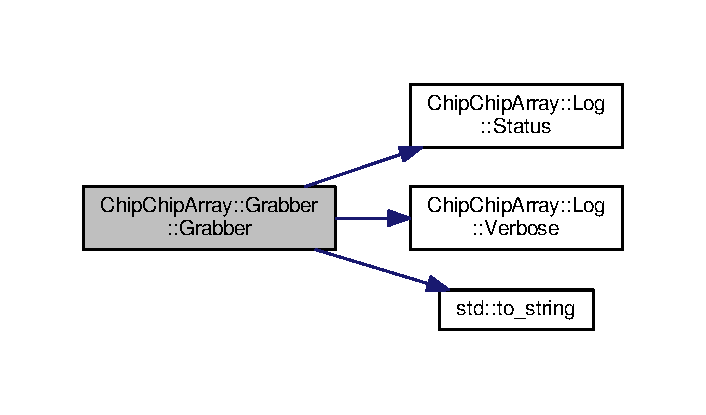
\includegraphics[width=339pt]{classChipChipArray_1_1Grabber_a7333f40c135fbe92d59651f75032b4e7_cgraph}
\end{center}
\end{figure}




\subsection{Member Function Documentation}
\hypertarget{classChipChipArray_1_1Grabber_aacf089ceb4aa5b263c2cc702fb3daf74}{\index{Chip\+Chip\+Array\+::\+Grabber@{Chip\+Chip\+Array\+::\+Grabber}!Close@{Close}}
\index{Close@{Close}!Chip\+Chip\+Array\+::\+Grabber@{Chip\+Chip\+Array\+::\+Grabber}}
\subsubsection[{Close}]{\setlength{\rightskip}{0pt plus 5cm}void Chip\+Chip\+Array\+::\+Grabber\+::\+Close (
\begin{DoxyParamCaption}
{}
\end{DoxyParamCaption}
)}}\label{classChipChipArray_1_1Grabber_aacf089ceb4aa5b263c2cc702fb3daf74}
Closes the \hyperlink{classChipChipArray_1_1Grabber}{Grabber}. Retracts the arm and closes the camera. 

Definition at line \hyperlink{Grabber_8hpp_source_l00166}{166} of file \hyperlink{Grabber_8hpp_source}{Grabber.\+hpp}.


\begin{DoxyCode}
00166                         \{
00167         log.\hyperlink{classChipChipArray_1_1Log_a66575b6e94c6112e4cefa5736cb996e0}{Status}(\textcolor{stringliteral}{"Closing Grabber"});
00168         \hyperlink{classChipChipArray_1_1Grabber_a726bcc2367a719cb84de92a981947622}{cam}.\hyperlink{classChipChipArray_1_1PiCamera_a38f8205921d6deec5a2c360ea7d24cc5}{Close}();
00169     \}
\end{DoxyCode}


Here is the call graph for this function\+:
\nopagebreak
\begin{figure}[H]
\begin{center}
\leavevmode
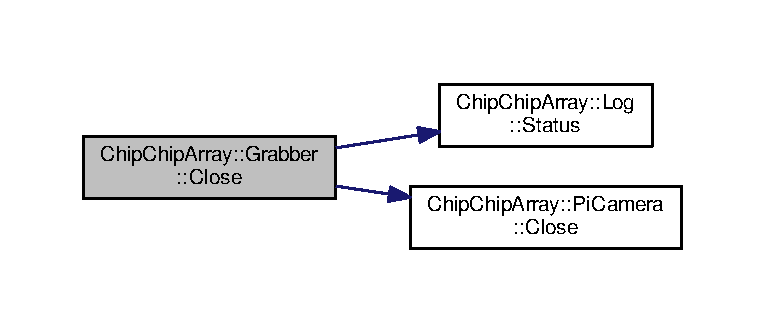
\includegraphics[width=350pt]{classChipChipArray_1_1Grabber_aacf089ceb4aa5b263c2cc702fb3daf74_cgraph}
\end{center}
\end{figure}




Here is the caller graph for this function\+:
\nopagebreak
\begin{figure}[H]
\begin{center}
\leavevmode
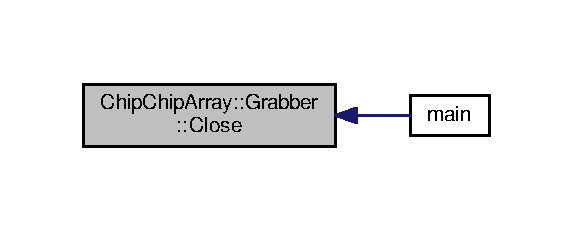
\includegraphics[width=275pt]{classChipChipArray_1_1Grabber_aacf089ceb4aa5b263c2cc702fb3daf74_icgraph}
\end{center}
\end{figure}


\hypertarget{classChipChipArray_1_1Grabber_a44e5aeb908634f68de356ad8df3c4bf1}{\index{Chip\+Chip\+Array\+::\+Grabber@{Chip\+Chip\+Array\+::\+Grabber}!Deposit@{Deposit}}
\index{Deposit@{Deposit}!Chip\+Chip\+Array\+::\+Grabber@{Chip\+Chip\+Array\+::\+Grabber}}
\subsubsection[{Deposit}]{\setlength{\rightskip}{0pt plus 5cm}void Chip\+Chip\+Array\+::\+Grabber\+::\+Deposit (
\begin{DoxyParamCaption}
\item[{{\bf Color}}]{color = {\ttfamily {\bf Color\+::\+Blue}}}
\end{DoxyParamCaption}
)\hspace{0.3cm}{\ttfamily [protected]}}}\label{classChipChipArray_1_1Grabber_a44e5aeb908634f68de356ad8df3c4bf1}
Deposits blocks in the storage/unloading unit. 

Definition at line \hyperlink{Grabber_8hpp_source_l00171}{171} of file \hyperlink{Grabber_8hpp_source}{Grabber.\+hpp}.


\begin{DoxyCode}
00171                                      \{
00172         \textcolor{keywordflow}{if}(color == \hyperlink{definitions_8hpp_abc05a0f46084a3477cf5d5c939ff1436a9594eec95be70e7b1710f730fdda33d9}{Color::Blue}) \{
00173             arm.\hyperlink{classChipChipArray_1_1Arm_a20c6fe3fe79c16f492a8c18b91427080}{ClawClose}();
00174             sleep(1);
00175             arm.\hyperlink{classChipChipArray_1_1Arm_a8b077a3791d9fc5ef285c1520fe4c5d8}{BaseTilt}(160);
00176             sleep(1);
00177             arm.\hyperlink{classChipChipArray_1_1Arm_ac45149e03abfac230b75156bb42e8417}{Elbow}(130);
00178             sleep(1);
00179             arm.\hyperlink{classChipChipArray_1_1Arm_addaedfe85ff2b14ff00c344fc4b40cd6}{BaseTurn}(47);
00180             sleep(1);
00181             arm.\hyperlink{classChipChipArray_1_1Arm_abb33b5bb11034554d632f8c9b95b2c44}{ClawOpen}();
00182             sleep(1);
00183         \} \textcolor{keywordflow}{else} \{
00184             \textcolor{keywordflow}{throw} std::runtime\_error(\textcolor{stringliteral}{"Du Idiot! Die Armbewegungen für diese "}
00185                     \textcolor{stringliteral}{"Farbe sind noch nicht implementiert. Vielleicht sollst "}
00186                     \textcolor{stringliteral}{"du die englische Phrase lernen 'Would you like fries "}
00187                     \textcolor{stringliteral}{"with that?"});
00188         \}
00189     \}
\end{DoxyCode}


Here is the call graph for this function\+:
\nopagebreak
\begin{figure}[H]
\begin{center}
\leavevmode
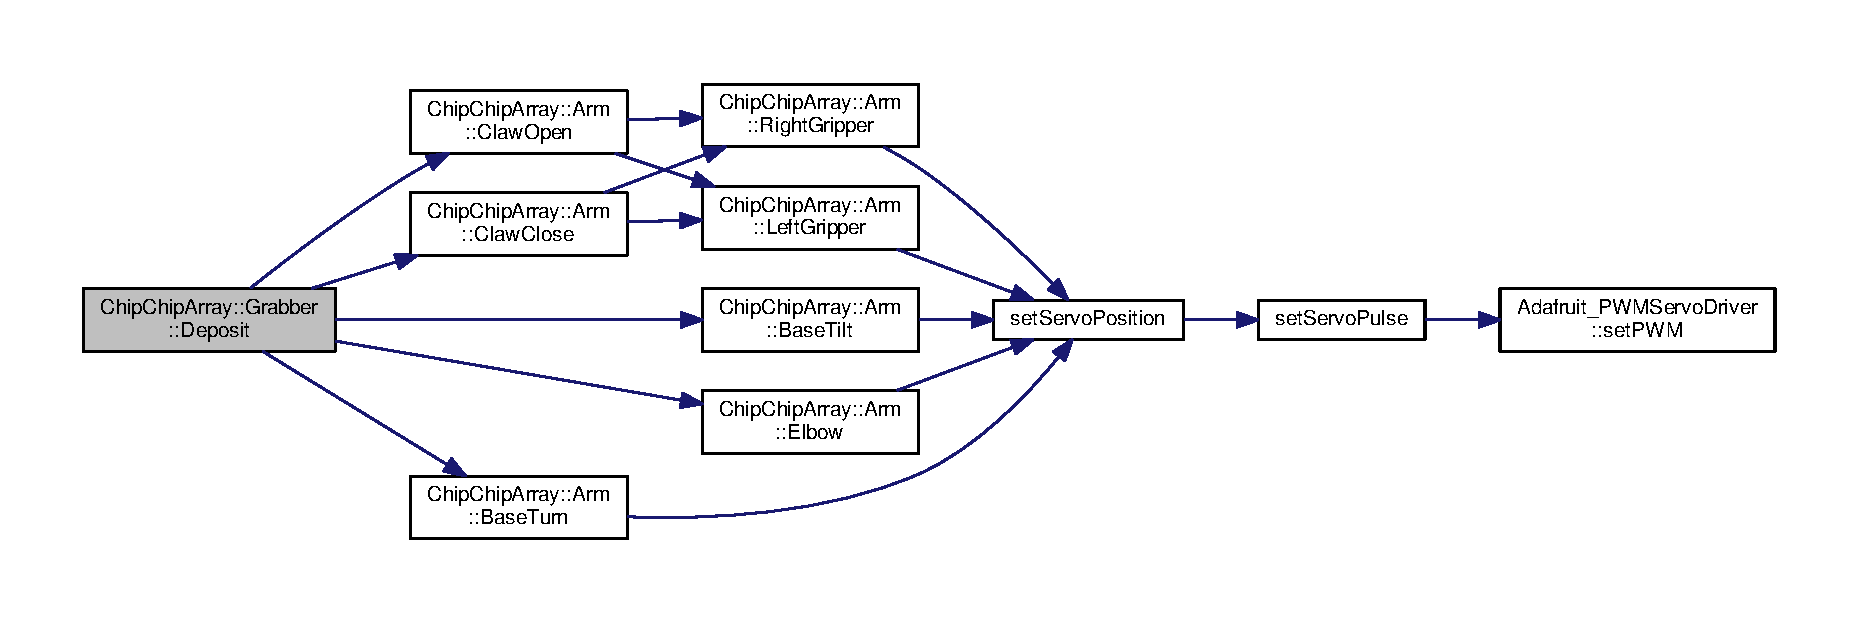
\includegraphics[width=350pt]{classChipChipArray_1_1Grabber_a44e5aeb908634f68de356ad8df3c4bf1_cgraph}
\end{center}
\end{figure}




Here is the caller graph for this function\+:
\nopagebreak
\begin{figure}[H]
\begin{center}
\leavevmode
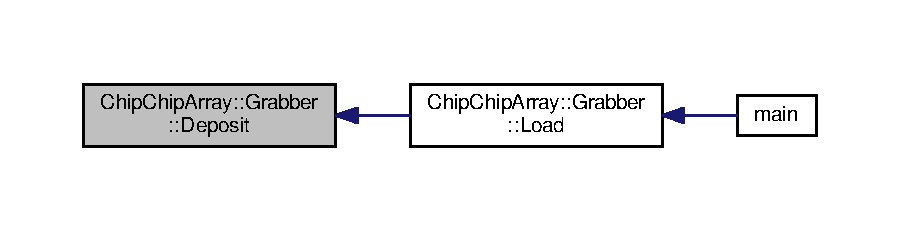
\includegraphics[width=350pt]{classChipChipArray_1_1Grabber_a44e5aeb908634f68de356ad8df3c4bf1_icgraph}
\end{center}
\end{figure}


\hypertarget{classChipChipArray_1_1Grabber_abecb4047b4f7d5a7e691b7fb581b5a39}{\index{Chip\+Chip\+Array\+::\+Grabber@{Chip\+Chip\+Array\+::\+Grabber}!Extend@{Extend}}
\index{Extend@{Extend}!Chip\+Chip\+Array\+::\+Grabber@{Chip\+Chip\+Array\+::\+Grabber}}
\subsubsection[{Extend}]{\setlength{\rightskip}{0pt plus 5cm}void Chip\+Chip\+Array\+::\+Grabber\+::\+Extend (
\begin{DoxyParamCaption}
{}
\end{DoxyParamCaption}
)\hspace{0.3cm}{\ttfamily [protected]}}}\label{classChipChipArray_1_1Grabber_abecb4047b4f7d5a7e691b7fb581b5a39}
Sets arm to generic position roughly right above a stack of blocks. 

Definition at line \hyperlink{Grabber_8hpp_source_l00191}{191} of file \hyperlink{Grabber_8hpp_source}{Grabber.\+hpp}.


\begin{DoxyCode}
00191                          \{
00192         arm.\hyperlink{classChipChipArray_1_1Arm_ac45149e03abfac230b75156bb42e8417}{Elbow}(180);
00193         usleep(500000);
00194         arm.\hyperlink{classChipChipArray_1_1Arm_addaedfe85ff2b14ff00c344fc4b40cd6}{BaseTurn}(132);
00195         arm.\hyperlink{classChipChipArray_1_1Arm_a8b077a3791d9fc5ef285c1520fe4c5d8}{BaseTilt}(125);
00196         arm.\hyperlink{classChipChipArray_1_1Arm_ac45149e03abfac230b75156bb42e8417}{Elbow}(150);
00197         arm.\hyperlink{classChipChipArray_1_1Arm_a35ec7756840d9d32dcfbb88d831f087f}{WristTwist}(90);
00198         arm.\hyperlink{classChipChipArray_1_1Arm_abb33b5bb11034554d632f8c9b95b2c44}{ClawOpen}();
00199         sleep(2);
00200     \}
\end{DoxyCode}


Here is the call graph for this function\+:
\nopagebreak
\begin{figure}[H]
\begin{center}
\leavevmode
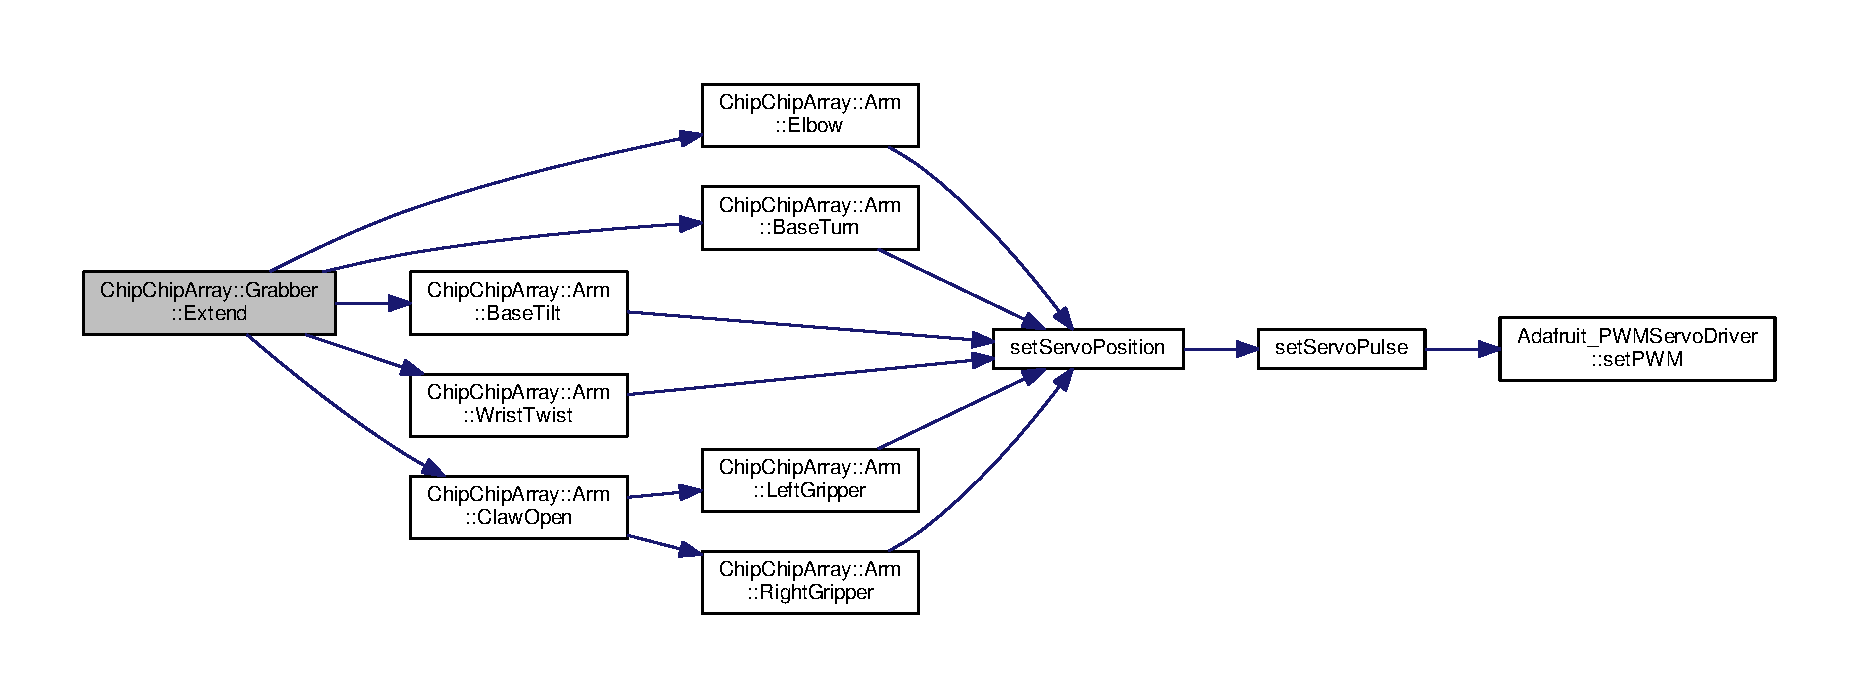
\includegraphics[width=350pt]{classChipChipArray_1_1Grabber_abecb4047b4f7d5a7e691b7fb581b5a39_cgraph}
\end{center}
\end{figure}




Here is the caller graph for this function\+:
\nopagebreak
\begin{figure}[H]
\begin{center}
\leavevmode
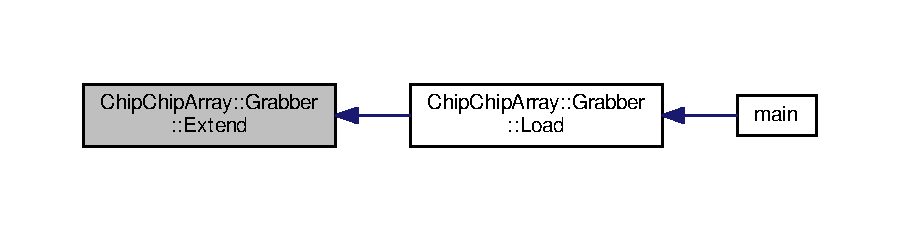
\includegraphics[width=350pt]{classChipChipArray_1_1Grabber_abecb4047b4f7d5a7e691b7fb581b5a39_icgraph}
\end{center}
\end{figure}


\hypertarget{classChipChipArray_1_1Grabber_a56639f8f9ba9468bce4b6d69ceb2eb54}{\index{Chip\+Chip\+Array\+::\+Grabber@{Chip\+Chip\+Array\+::\+Grabber}!Load@{Load}}
\index{Load@{Load}!Chip\+Chip\+Array\+::\+Grabber@{Chip\+Chip\+Array\+::\+Grabber}}
\subsubsection[{Load}]{\setlength{\rightskip}{0pt plus 5cm}{\bf Result} Chip\+Chip\+Array\+::\+Grabber\+::\+Load (
\begin{DoxyParamCaption}
{}
\end{DoxyParamCaption}
)}}\label{classChipChipArray_1_1Grabber_a56639f8f9ba9468bce4b6d69ceb2eb54}
Loads a block(s) (if possible) at the robot's current position.

\begin{DoxyReturn}{Returns}
the number of half and whole blocks loaded 
\end{DoxyReturn}


Definition at line \hyperlink{Grabber_8hpp_source_l00202}{202} of file \hyperlink{Grabber_8hpp_source}{Grabber.\+hpp}.


\begin{DoxyCode}
00202                          \{
00203         \textcolor{keywordflow}{for}(\hyperlink{definitions_8hpp_adde6aaee8457bee49c2a92621fe22b79}{uint8} i = 0; i < 2; i++) \{
00204             \hyperlink{classChipChipArray_1_1Grabber_abecb4047b4f7d5a7e691b7fb581b5a39}{Extend}();
00205 
00206             \textcolor{keywordflow}{try} \{
00207                 Block block = (\hyperlink{classChipChipArray_1_1Grabber_ab57efe6e0b6f369b19528285a278d967}{zone} == \hyperlink{definitions_8hpp_adbd1e7a33d3e1751c7b2aa2562d0ecb9a7fc56270e7a70fa81a5935b72eacbe29}{Zone::A})
00208                     ? \hyperlink{classChipChipArray_1_1Grabber_af49248c957a1695dcde79c0f5f8df99b}{LocateBlocks}(\hyperlink{definitions_8hpp_abc05a0f46084a3477cf5d5c939ff1436a9594eec95be70e7b1710f730fdda33d9}{Color::Blue}) : 
      \hyperlink{classChipChipArray_1_1Grabber_ab9b0d6a64b2c94c0d0f810a5ebeef6ec}{LocateBlueBlock}();
00209 
00210                 \hyperlink{definitions_8hpp_aacdc525d6f7bddb3ae95d5c311bd06a1}{float32} baseKonstant = 0.5;
00211                 \textcolor{keywordflow}{if}(block.dRightLeft > 0) baseKonstant *= -1;
00212                 \hyperlink{definitions_8hpp_aacdc525d6f7bddb3ae95d5c311bd06a1}{float32} degree = baseKonstant * std::sqrt(block.dRightLeft);
00213                 arm.\hyperlink{classChipChipArray_1_1Arm_a980f5bd278cbe06aa21754fb8e0324b3}{dBaseTurn}(degree);
00214                 arm.\hyperlink{classChipChipArray_1_1Arm_a6bde822b1be63926e21222f36aad67b3}{dWristTwist}(-degree);
00215                 sleep(1);
00216                 arm.\hyperlink{classChipChipArray_1_1Arm_a8b077a3791d9fc5ef285c1520fe4c5d8}{BaseTilt}(140);
00217                 sleep(1);
00218 
00219                 \hyperlink{definitions_8hpp_adde6aaee8457bee49c2a92621fe22b79}{uint8} bend = (i == 0 ? 100 : 90);
00220 
00221                 \textcolor{comment}{// lower claw over block}
00222                 \textcolor{keywordflow}{for}(\hyperlink{definitions_8hpp_adde6aaee8457bee49c2a92621fe22b79}{uint8} j = 140; j >= bend; j -= 10) \{
00223                     arm.\hyperlink{classChipChipArray_1_1Arm_ac45149e03abfac230b75156bb42e8417}{Elbow}(j);
00224                     sleep(1);
00225                 \}
00226 
00227                 \textcolor{comment}{// deposit in bin}
00228                 sleep(1);
00229                 \hyperlink{classChipChipArray_1_1Grabber_a44e5aeb908634f68de356ad8df3c4bf1}{Deposit}();
00230             \} \textcolor{keywordflow}{catch}(std::exception ex) \{
00231                 log.\hyperlink{classChipChipArray_1_1Log_aba7b7b0555f49f4dcf15f4b9fd3e6b34}{Error}(std::string(\textcolor{stringliteral}{"An exception occured attempting "}
00232                             \textcolor{stringliteral}{"to load the blocks in function Grabber::Load(): "}) 
00233                         + ex.what());
00234             \}
00235 
00236 
00237             \textcolor{keywordflow}{if}(i == 0) \{
00238                 arm.\hyperlink{classChipChipArray_1_1Arm_addaedfe85ff2b14ff00c344fc4b40cd6}{BaseTurn}(132);
00239             \} \textcolor{keywordflow}{else} \{
00240                 arm.\hyperlink{classChipChipArray_1_1Arm_addaedfe85ff2b14ff00c344fc4b40cd6}{BaseTurn}(135);
00241                 sleep(1);
00242                 arm.\hyperlink{classChipChipArray_1_1Arm_a8b077a3791d9fc5ef285c1520fe4c5d8}{BaseTilt}(180);
00243                 sleep(1);
00244                 arm.\hyperlink{classChipChipArray_1_1Arm_ac45149e03abfac230b75156bb42e8417}{Elbow}(90);
00245                 sleep(1);
00246                 arm.\hyperlink{classChipChipArray_1_1Arm_ac45149e03abfac230b75156bb42e8417}{Elbow}(45);
00247                 sleep(1);
00248                 arm.\hyperlink{classChipChipArray_1_1Arm_ac45149e03abfac230b75156bb42e8417}{Elbow}(0);
00249             \}
00250         \}
00251     \}
\end{DoxyCode}


Here is the call graph for this function\+:
\nopagebreak
\begin{figure}[H]
\begin{center}
\leavevmode
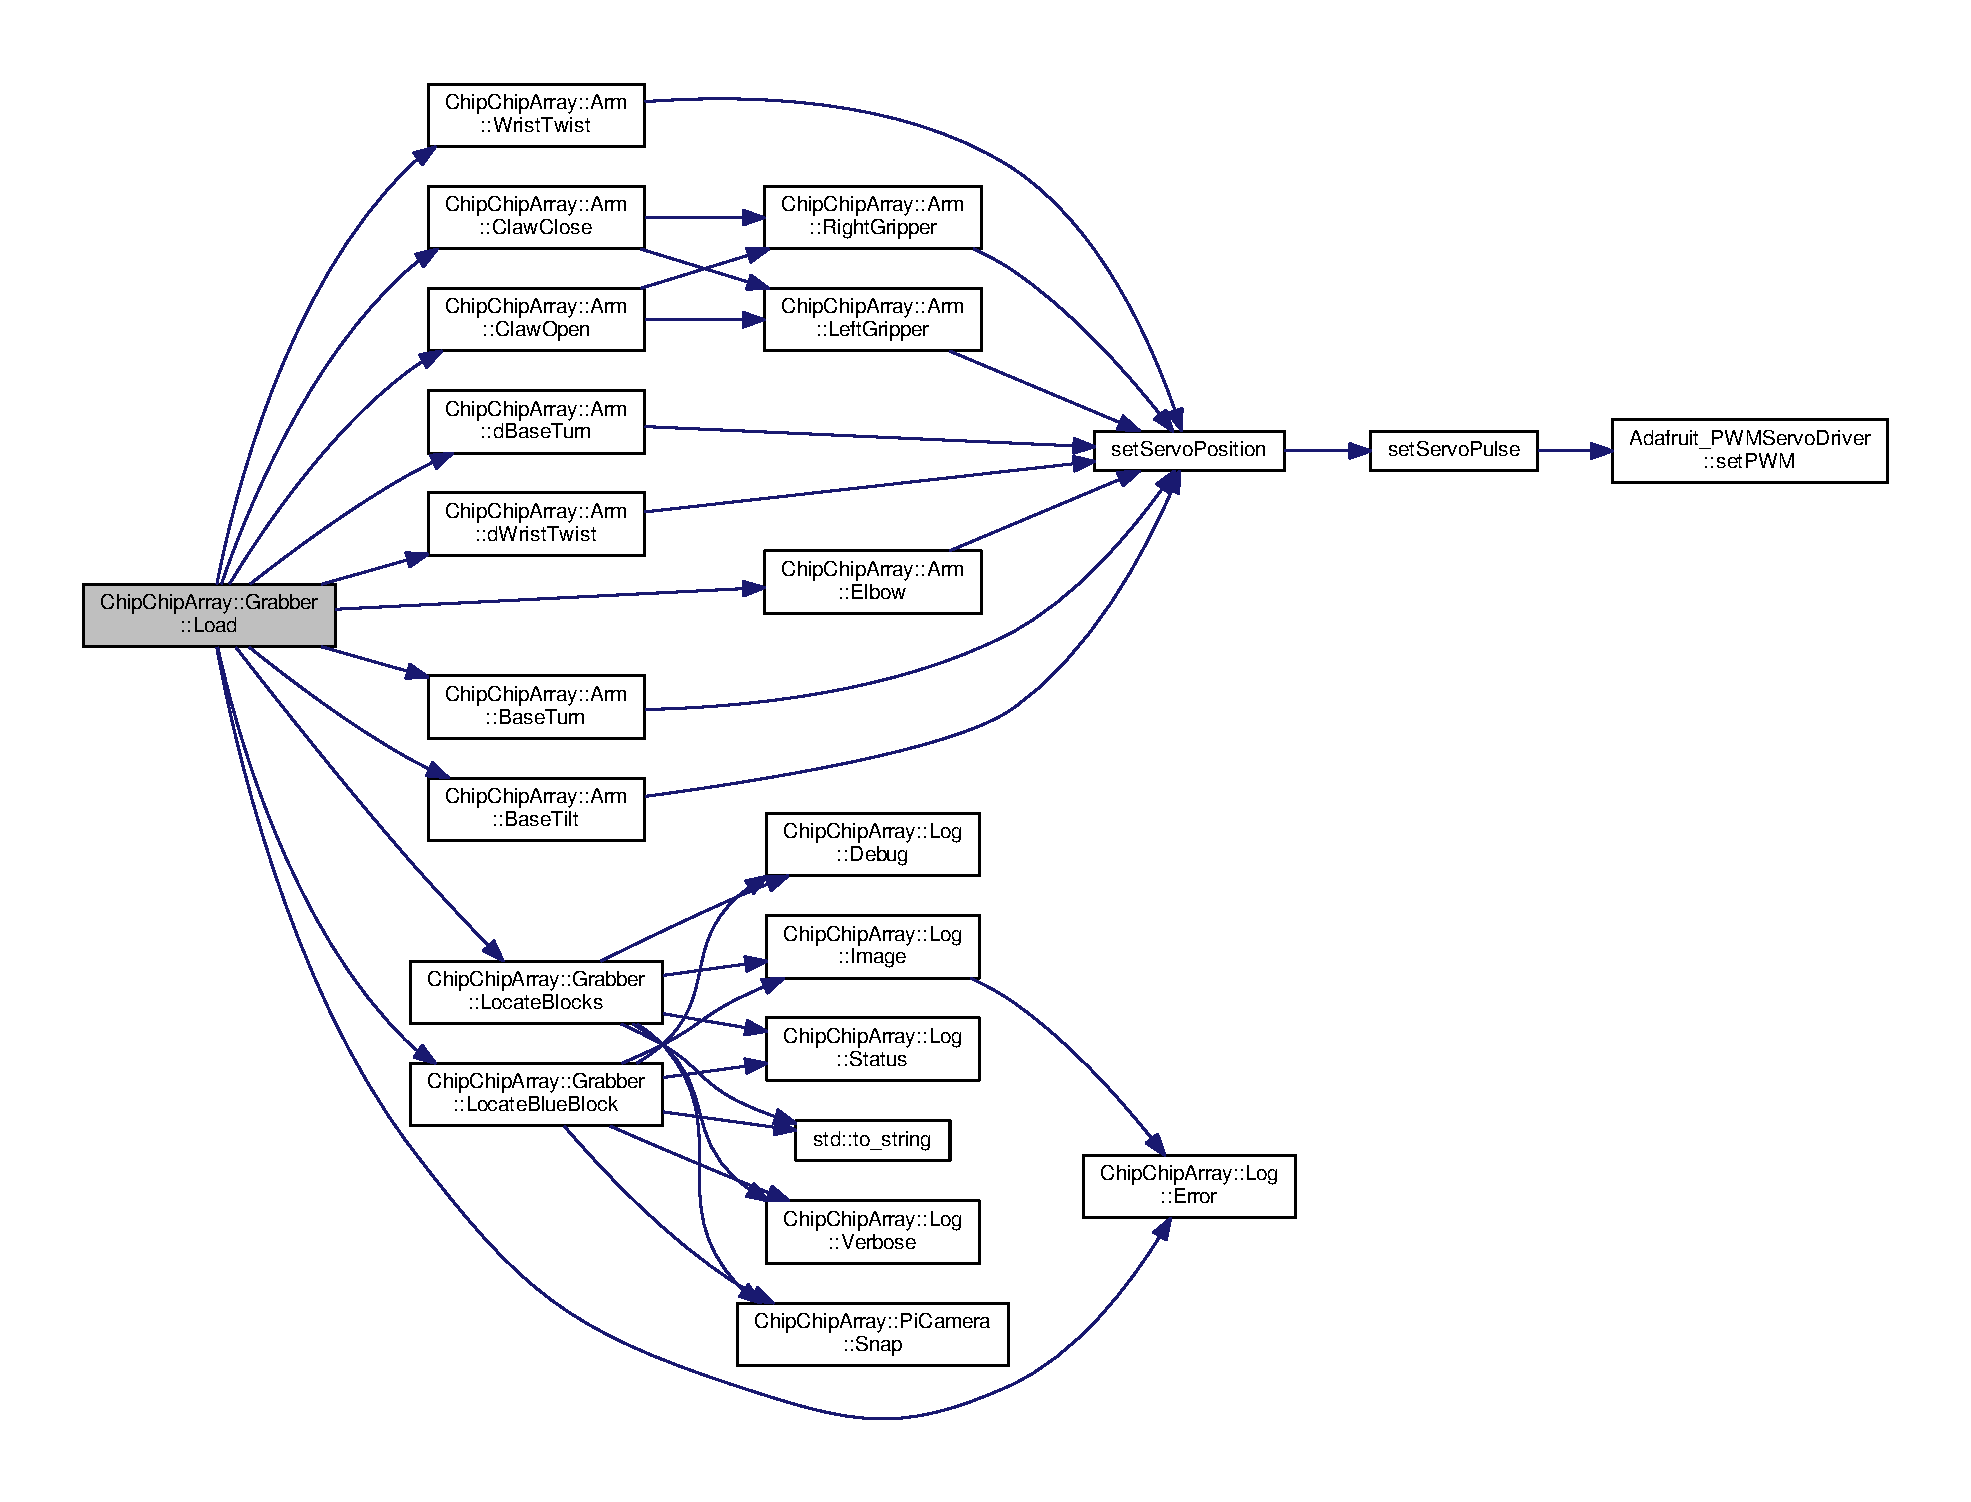
\includegraphics[width=350pt]{classChipChipArray_1_1Grabber_a56639f8f9ba9468bce4b6d69ceb2eb54_cgraph}
\end{center}
\end{figure}




Here is the caller graph for this function\+:
\nopagebreak
\begin{figure}[H]
\begin{center}
\leavevmode
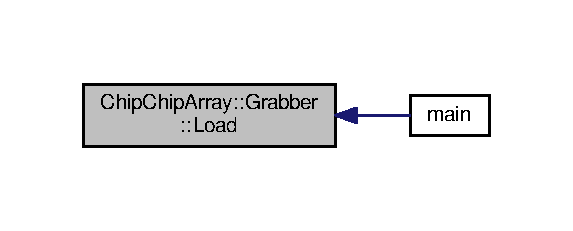
\includegraphics[width=275pt]{classChipChipArray_1_1Grabber_a56639f8f9ba9468bce4b6d69ceb2eb54_icgraph}
\end{center}
\end{figure}


\hypertarget{classChipChipArray_1_1Grabber_af49248c957a1695dcde79c0f5f8df99b}{\index{Chip\+Chip\+Array\+::\+Grabber@{Chip\+Chip\+Array\+::\+Grabber}!Locate\+Blocks@{Locate\+Blocks}}
\index{Locate\+Blocks@{Locate\+Blocks}!Chip\+Chip\+Array\+::\+Grabber@{Chip\+Chip\+Array\+::\+Grabber}}
\subsubsection[{Locate\+Blocks}]{\setlength{\rightskip}{0pt plus 5cm}{\bf Block} Chip\+Chip\+Array\+::\+Grabber\+::\+Locate\+Blocks (
\begin{DoxyParamCaption}
\item[{{\bf Color}}]{color = {\ttfamily {\bf Color\+::\+Perrywinkle}}}
\end{DoxyParamCaption}
)\hspace{0.3cm}{\ttfamily [protected]}}}\label{classChipChipArray_1_1Grabber_af49248c957a1695dcde79c0f5f8df99b}
Loads a stack of blocks for all zones. Does multiple colors and both sizes.


\begin{DoxyParams}{Parameters}
{\em color} & the color block for which to search. Perrywinkle denotes searching for all colors (because who actually knows what color perrywinkle is?).\\
\hline
\end{DoxyParams}
\begin{DoxyReturn}{Returns}
\hyperlink{classChipChipArray_1_1Block}{Block} instance representing the block found 
\end{DoxyReturn}


Definition at line \hyperlink{Grabber_8hpp_source_l00254}{254} of file \hyperlink{Grabber_8hpp_source}{Grabber.\+hpp}.


\begin{DoxyCode}
00254                                            \{
00255         invokeCount++;
00256         std::string logstr = \textcolor{stringliteral}{"Locating blocks"};
00257 
00258         \textcolor{keywordflow}{if}(color == \hyperlink{definitions_8hpp_abc05a0f46084a3477cf5d5c939ff1436a1e700ac224a6d34c5b171bb6f462aa41}{Color::Perrywinkle}) \{
00259             logstr += \textcolor{stringliteral}{" ("} + \hyperlink{namespacestd_aa5ddf582a1c96ffe258c997be9a294a3}{std::to\_string}(color) + \textcolor{stringliteral}{")"};
00260         \}
00261 
00262         log.\hyperlink{classChipChipArray_1_1Log_a154a5f38d9c7a767693b242684a3d4d9}{Verbose}(logstr);
00263 
00264         cv::Mat imgOrig;
00265         cv::transpose(\hyperlink{classChipChipArray_1_1Grabber_a726bcc2367a719cb84de92a981947622}{cam}.\hyperlink{classChipChipArray_1_1PiCamera_a58fb0de02570dce9a9cb60a1a04fb84f}{Snap}(), imgOrig);
00266 
00267         cv::Mat imgHSV;
00268         cv::Mat imgThresh;
00269         std::vector<cv::Rect> blocks;
00270         std::vector<Color> colors;
00271 
00272         \hyperlink{definitions_8hpp_adde6aaee8457bee49c2a92621fe22b79}{uint8} loopNum = (color == \hyperlink{definitions_8hpp_abc05a0f46084a3477cf5d5c939ff1436a1e700ac224a6d34c5b171bb6f462aa41}{Color::Perrywinkle} ? rangeVals.size() : 1);
00273 
00274         \textcolor{keywordflow}{for}(\textcolor{keywordtype}{int} i = 0; i < loopNum; i++) \{
00275             \textcolor{keywordflow}{if}(loopNum > 1) \{
00276                 \textcolor{keywordflow}{switch}(i) \{
00277                     \textcolor{keywordflow}{case} 0:
00278                         color = \hyperlink{definitions_8hpp_abc05a0f46084a3477cf5d5c939ff1436aee38e4d5dd68c4e440825018d549cb47}{Color::Red};
00279                         \textcolor{keywordflow}{break};
00280 
00281                     \textcolor{keywordflow}{case} 1:
00282                         color = \hyperlink{definitions_8hpp_abc05a0f46084a3477cf5d5c939ff1436ad382816a3cbeed082c9e216e7392eed1}{Color::Green};
00283                         \textcolor{keywordflow}{break};
00284 
00285                     \textcolor{keywordflow}{case} 2:
00286                         color = \hyperlink{definitions_8hpp_abc05a0f46084a3477cf5d5c939ff1436a9594eec95be70e7b1710f730fdda33d9}{Color::Blue};
00287                         \textcolor{keywordflow}{break};
00288 
00289                         \textcolor{comment}{/* Must be last, because it changes imgHSV from HSV space}
00290 \textcolor{comment}{                         * to YUV space. */}
00291                     \textcolor{keywordflow}{case} 3: 
00292                         color = \hyperlink{definitions_8hpp_abc05a0f46084a3477cf5d5c939ff1436a51e6cd92b6c45f9affdc158ecca2b8b8}{Color::Yellow};
00293                         \textcolor{keywordflow}{break};
00294                 \}
00295             \}
00296 
00297             log.\hyperlink{classChipChipArray_1_1Log_a154a5f38d9c7a767693b242684a3d4d9}{Verbose}(\textcolor{stringliteral}{"Searching: "} + \hyperlink{namespacestd_aa5ddf582a1c96ffe258c997be9a294a3}{std::to\_string}(color));
00298 
00299             \textcolor{keywordflow}{if}(color == \hyperlink{definitions_8hpp_abc05a0f46084a3477cf5d5c939ff1436a51e6cd92b6c45f9affdc158ecca2b8b8}{Color::Yellow}) \{
00300                 cv::Mat temp;
00301                 imgOrig.copyTo(temp);
00302                 cv::cvtColor(imgOrig, imgHSV, CV\_BGR2YUV);
00303                 cv::cvtColor(imgHSV, temp, CV\_HSV2BGR);
00304                 cv::cvtColor(temp, imgHSV, cv::COLOR\_BGR2HSV);
00305                 log.\hyperlink{classChipChipArray_1_1Log_a65bbab057c8b1453f9e4efcfee7522c4}{Image}(temp, \textcolor{stringliteral}{"yuv\_yellow\_"} + \hyperlink{namespacestd_aa5ddf582a1c96ffe258c997be9a294a3}{std::to\_string}(color)
00306                         + \textcolor{stringliteral}{"\_"} + \hyperlink{namespacestd_aa5ddf582a1c96ffe258c997be9a294a3}{std::to\_string}(\hyperlink{classChipChipArray_1_1Grabber_ab57efe6e0b6f369b19528285a278d967}{zone})
00307                         + \hyperlink{namespacestd_aa5ddf582a1c96ffe258c997be9a294a3}{std::to\_string}(invokeCount)
00308                         + \textcolor{stringliteral}{".bmp"});
00309             \} \textcolor{keywordflow}{else} \{
00310                 cv::cvtColor(imgOrig, imgHSV, cv::COLOR\_BGR2HSV);
00311             \}
00312 
00313             cv::inRange(imgHSV, rangeVals[color][0],
00314                     rangeVals[color][1], imgThresh);
00315 
00316             \textcolor{comment}{/* }
00317 \textcolor{comment}{             * Not quite sure what all this does, but it seems to}
00318 \textcolor{comment}{             * relate to smoothing the image}
00319 \textcolor{comment}{             */}
00320             cv::erode(imgThresh, imgThresh,
00321                     cv::getStructuringElement(
00322                         cv::MORPH\_ELLIPSE,
00323                         \hyperlink{definitions_8hpp_a9809446fd16a744b6df9808293f14153}{cv::Size}(5, 5)));
00324             cv::dilate(imgThresh, imgThresh,
00325                     cv::getStructuringElement(
00326                         cv::MORPH\_ELLIPSE,
00327                         \hyperlink{definitions_8hpp_a9809446fd16a744b6df9808293f14153}{cv::Size}(5, 5)));
00328             cv::dilate(imgThresh, imgThresh,
00329                     cv::getStructuringElement(
00330                         cv::MORPH\_ELLIPSE,
00331                         \hyperlink{definitions_8hpp_a9809446fd16a744b6df9808293f14153}{cv::Size}(5, 5)));
00332             cv::erode(imgThresh, imgThresh,
00333                     cv::getStructuringElement(
00334                         cv::MORPH\_ELLIPSE,
00335                         \hyperlink{definitions_8hpp_a9809446fd16a744b6df9808293f14153}{cv::Size}(5, 5)));
00336 
00337             log.\hyperlink{classChipChipArray_1_1Log_a65bbab057c8b1453f9e4efcfee7522c4}{Image}(imgThresh, \textcolor{stringliteral}{"thresh\_"} + \hyperlink{namespacestd_aa5ddf582a1c96ffe258c997be9a294a3}{std::to\_string}(color)
00338                     + \textcolor{stringliteral}{"\_"} + \hyperlink{namespacestd_aa5ddf582a1c96ffe258c997be9a294a3}{std::to\_string}(\hyperlink{classChipChipArray_1_1Grabber_ab57efe6e0b6f369b19528285a278d967}{zone})
00339                     + \hyperlink{namespacestd_aa5ddf582a1c96ffe258c997be9a294a3}{std::to\_string}(invokeCount)
00340                     + \textcolor{stringliteral}{".bmp"});
00341 
00342             \textcolor{comment}{// calculate contours}
00343             std::vector<std::vector<cv::Point>> contours;
00344             cv::findContours(imgThresh, contours, CV\_RETR\_TREE,
00345                     CV\_CHAIN\_APPROX\_SIMPLE,
00346                     cv::Point(0, 0));
00347             std::vector<std::vector<cv::Point>>
00348                 contours\_poly(contours.size());
00349             std::vector<cv::Rect> bounds(contours.size());
00350 
00351             \textcolor{comment}{// find rectangle around polygon-ish shapes}
00352             \textcolor{keywordflow}{for}(\textcolor{keywordtype}{int} i = 0; i < contours.size(); i++) \{
00353                 \hyperlink{definitions_8hpp_a1134b580f8da4de94ca6b1de4d37975e}{uint32} area = cv::contourArea(contours[i]);
00354 
00355                 \textcolor{comment}{// determine if block and add to blocks vector}
00356                 \textcolor{keywordflow}{if}(area > MIN\_HALF\_BLOCK\_SIZE) \{
00357                     cv::approxPolyDP(cv::Mat(contours[i]),
00358                             contours\_poly[i], 20,
00359                             \textcolor{keyword}{false});
00360                     cv::Rect rect = cv::boundingRect(
00361                             cv::Mat(contours\_poly[i]));
00362                     log.\hyperlink{classChipChipArray_1_1Log_ac32b435af1577e4ebc67af2bdfea8eff}{Debug}(\hyperlink{namespacestd_aa5ddf582a1c96ffe258c997be9a294a3}{std::to\_string}(color)
00363                             + \textcolor{stringliteral}{" block detected "}
00364                             \textcolor{stringliteral}{"with area "}
00365                             + \hyperlink{namespacestd_aa5ddf582a1c96ffe258c997be9a294a3}{std::to\_string}(
00366                                 area));
00367                     blocks.push\_back(rect);
00368                     colors.push\_back(color);
00369                 \}
00370             \}
00371         \}
00372 
00373         \textcolor{keywordflow}{if}(blocks.size() == 0) \{
00374             log.\hyperlink{classChipChipArray_1_1Log_a65bbab057c8b1453f9e4efcfee7522c4}{Image}(imgOrig, \textcolor{stringliteral}{"original\_"} + \hyperlink{namespacestd_aa5ddf582a1c96ffe258c997be9a294a3}{std::to\_string}(
      \hyperlink{classChipChipArray_1_1Grabber_ab57efe6e0b6f369b19528285a278d967}{zone})
00375                     + \hyperlink{namespacestd_aa5ddf582a1c96ffe258c997be9a294a3}{std::to\_string}(invokeCount)
00376                     + \textcolor{stringliteral}{"\_no\_blocks.bmp"});
00377             \textcolor{keywordflow}{throw} std::runtime\_error(\textcolor{stringliteral}{"No blocks found!"});
00378         \} \textcolor{keywordflow}{else} \{
00379             log.\hyperlink{classChipChipArray_1_1Log_a66575b6e94c6112e4cefa5736cb996e0}{Status}(\hyperlink{namespacestd_aa5ddf582a1c96ffe258c997be9a294a3}{std::to\_string}(blocks.size())
00380                     + \textcolor{stringliteral}{" blocks found"});
00381         \}
00382 
00383         \textcolor{comment}{// coordinates start in top right}
00384         Block block = Block(blocks[0], colors[0]);
00385 
00386         \textcolor{keywordflow}{if}(blocks.size() > 1) \{
00387             \textcolor{keywordflow}{for}(\textcolor{keywordtype}{int} i = 1; i < blocks.size(); i++) \{ 
00388                 \textcolor{keywordflow}{if}((\hyperlink{classChipChipArray_1_1Grabber_a8afbaefae7c767c862fd1bf13968539b}{side} == \hyperlink{definitions_8hpp_a03325a8a9d4f105db5e37dd587128142a92b09c7c48c520c3c55e497875da437c}{Side::Right} && blocks[i].x 
00389                             > block.topLeft.x)
00390                         || (\hyperlink{classChipChipArray_1_1Grabber_a8afbaefae7c767c862fd1bf13968539b}{side} == \hyperlink{definitions_8hpp_a03325a8a9d4f105db5e37dd587128142a945d5e233cf7d6240f6b783b36a374ff}{Side::Left}
00391                             && blocks[i].x
00392                             < block.topLeft.x)) \{
00393                     block = Block(blocks[i], colors[i]);
00394                 \}
00395             \}
00396         \}
00397 
00398         log.\hyperlink{classChipChipArray_1_1Log_a66575b6e94c6112e4cefa5736cb996e0}{Status}(\hyperlink{namespacestd_aa5ddf582a1c96ffe258c997be9a294a3}{std::to\_string}(block.color) + \textcolor{stringliteral}{" block is located"});
00399 
00400         log.\hyperlink{classChipChipArray_1_1Log_ac32b435af1577e4ebc67af2bdfea8eff}{Debug}(\textcolor{stringliteral}{"Block properties => area: "} + \hyperlink{namespacestd_aa5ddf582a1c96ffe258c997be9a294a3}{std::to\_string}(block.area)
00401                 + \textcolor{stringliteral}{", height: "} + \hyperlink{namespacestd_aa5ddf582a1c96ffe258c997be9a294a3}{std::to\_string}(block.height) + \textcolor{stringliteral}{", width: "}
00402                 + \hyperlink{namespacestd_aa5ddf582a1c96ffe258c997be9a294a3}{std::to\_string}(block.width) + \textcolor{stringliteral}{", offset: "}
00403                 + \hyperlink{namespacestd_aa5ddf582a1c96ffe258c997be9a294a3}{std::to\_string}(block.offset) + \textcolor{stringliteral}{", color: "}
00404                 + \hyperlink{namespacestd_aa5ddf582a1c96ffe258c997be9a294a3}{std::to\_string}(block.color) + \textcolor{stringliteral}{", size: "}
00405                 + \hyperlink{namespacestd_aa5ddf582a1c96ffe258c997be9a294a3}{std::to\_string}(block.size));
00406 
00407         \textcolor{comment}{/* }
00408 \textcolor{comment}{         * Draw surrounding rectangles from above on original}
00409 \textcolor{comment}{         * image.}
00410 \textcolor{comment}{         */}
00411         cv::rectangle(imgOrig, block.topLeft , block.bottomRight,
00412                 cv::Scalar(255, 0, 0), 4, 8);
00413         log.\hyperlink{classChipChipArray_1_1Log_a65bbab057c8b1453f9e4efcfee7522c4}{Image}(imgOrig, \textcolor{stringliteral}{"original\_"} + \hyperlink{namespacestd_aa5ddf582a1c96ffe258c997be9a294a3}{std::to\_string}(\hyperlink{classChipChipArray_1_1Grabber_ab57efe6e0b6f369b19528285a278d967}{zone})
00414                 + \hyperlink{namespacestd_aa5ddf582a1c96ffe258c997be9a294a3}{std::to\_string}(invokeCount)
00415                 + \textcolor{stringliteral}{".bmp"});
00416 
00417         \textcolor{keywordflow}{return} block;
00418     \}
\end{DoxyCode}


Here is the call graph for this function\+:
\nopagebreak
\begin{figure}[H]
\begin{center}
\leavevmode
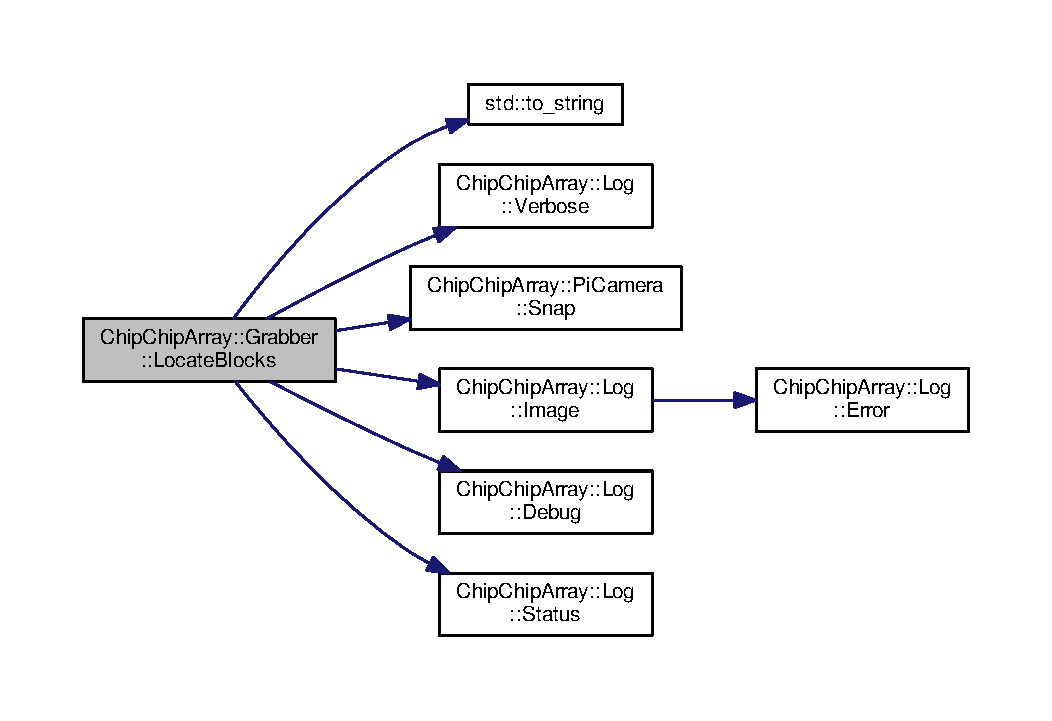
\includegraphics[width=350pt]{classChipChipArray_1_1Grabber_af49248c957a1695dcde79c0f5f8df99b_cgraph}
\end{center}
\end{figure}




Here is the caller graph for this function\+:
\nopagebreak
\begin{figure}[H]
\begin{center}
\leavevmode
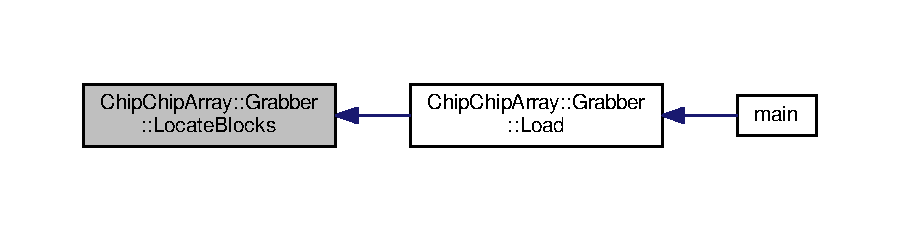
\includegraphics[width=350pt]{classChipChipArray_1_1Grabber_af49248c957a1695dcde79c0f5f8df99b_icgraph}
\end{center}
\end{figure}


\hypertarget{classChipChipArray_1_1Grabber_ab9b0d6a64b2c94c0d0f810a5ebeef6ec}{\index{Chip\+Chip\+Array\+::\+Grabber@{Chip\+Chip\+Array\+::\+Grabber}!Locate\+Blue\+Block@{Locate\+Blue\+Block}}
\index{Locate\+Blue\+Block@{Locate\+Blue\+Block}!Chip\+Chip\+Array\+::\+Grabber@{Chip\+Chip\+Array\+::\+Grabber}}
\subsubsection[{Locate\+Blue\+Block}]{\setlength{\rightskip}{0pt plus 5cm}{\bf Block} Chip\+Chip\+Array\+::\+Grabber\+::\+Locate\+Blue\+Block (
\begin{DoxyParamCaption}
{}
\end{DoxyParamCaption}
)\hspace{0.3cm}{\ttfamily [protected]}}}\label{classChipChipArray_1_1Grabber_ab9b0d6a64b2c94c0d0f810a5ebeef6ec}
Finds whole, blue blocks.

\begin{DoxyReturn}{Returns}
\hyperlink{classChipChipArray_1_1Block}{Block} instance representing the block found 
\end{DoxyReturn}


Definition at line \hyperlink{Grabber_8hpp_source_l00420}{420} of file \hyperlink{Grabber_8hpp_source}{Grabber.\+hpp}.


\begin{DoxyCode}
00420                                    \{
00421         std::vector<cv::Mat> channels;
00422         std::vector<cv::Rect> blocks;   
00423 
00424         invokeCount++;
00425         log.\hyperlink{classChipChipArray_1_1Log_a66575b6e94c6112e4cefa5736cb996e0}{Status}(\textcolor{stringliteral}{"Locating blue blocks"});
00426 
00427         cv::Mat img;
00428         cv::Mat imgThresh;
00429         cv::split(\hyperlink{classChipChipArray_1_1Grabber_a726bcc2367a719cb84de92a981947622}{cam}.\hyperlink{classChipChipArray_1_1PiCamera_a58fb0de02570dce9a9cb60a1a04fb84f}{Snap}(), channels);
00430         cv::transpose(channels[0], img);
00431 
00432         log.\hyperlink{classChipChipArray_1_1Log_a154a5f38d9c7a767693b242684a3d4d9}{Verbose}(\textcolor{stringliteral}{"Searching: Blue block"});
00433         cv::inRange(img, 30, 255, imgThresh);
00434         log.\hyperlink{classChipChipArray_1_1Log_a65bbab057c8b1453f9e4efcfee7522c4}{Image}(imgThresh, \textcolor{stringliteral}{"thresh\_blue"} + \hyperlink{namespacestd_aa5ddf582a1c96ffe258c997be9a294a3}{std::to\_string}(
      \hyperlink{classChipChipArray_1_1Grabber_ab57efe6e0b6f369b19528285a278d967}{zone})
00435                 + \hyperlink{namespacestd_aa5ddf582a1c96ffe258c997be9a294a3}{std::to\_string}(invokeCount) + \textcolor{stringliteral}{".bmp"});
00436 
00437         \textcolor{comment}{// calculate contours}
00438         std::vector<std::vector<cv::Point>> contours;
00439         cv::findContours(imgThresh, contours, CV\_RETR\_TREE,
00440                 CV\_CHAIN\_APPROX\_SIMPLE,
00441                 cv::Point(0, 0));
00442         std::vector<std::vector<cv::Point>>
00443             contours\_poly(contours.size());
00444         std::vector<cv::Rect> bounds(contours.size());
00445 
00446         \textcolor{comment}{// find rectangle around polygon-ish shapes}
00447         \textcolor{keywordflow}{for}(\textcolor{keywordtype}{int} i = 0; i < contours.size(); i++) \{
00448             \hyperlink{definitions_8hpp_a1134b580f8da4de94ca6b1de4d37975e}{uint32} area = cv::contourArea(contours[i]);
00449 
00450             \textcolor{comment}{// determine if block and add to blocks vector}
00451             \textcolor{keywordflow}{if}(area > MIN\_HALF\_BLOCK\_SIZE) \{
00452                 cv::approxPolyDP(cv::Mat(contours[i]),
00453                         contours\_poly[i], 20,
00454                         \textcolor{keyword}{false});
00455                 cv::Rect rect = cv::boundingRect(
00456                         cv::Mat(contours\_poly[i]));
00457                 log.\hyperlink{classChipChipArray_1_1Log_ac32b435af1577e4ebc67af2bdfea8eff}{Debug}(\textcolor{stringliteral}{"Blue block detected with area "}
00458                         + \hyperlink{namespacestd_aa5ddf582a1c96ffe258c997be9a294a3}{std::to\_string}(area));
00459                 blocks.push\_back(rect);
00460             \}
00461         \}
00462 
00463 
00464         \textcolor{keywordflow}{if}(blocks.size() == 0) \{
00465             log.\hyperlink{classChipChipArray_1_1Log_a65bbab057c8b1453f9e4efcfee7522c4}{Image}(img, \textcolor{stringliteral}{"original\_"} + \hyperlink{namespacestd_aa5ddf582a1c96ffe258c997be9a294a3}{std::to\_string}(\hyperlink{classChipChipArray_1_1Grabber_ab57efe6e0b6f369b19528285a278d967}{zone})
00466                     + \hyperlink{namespacestd_aa5ddf582a1c96ffe258c997be9a294a3}{std::to\_string}(invokeCount)
00467                     + \textcolor{stringliteral}{"\_no\_blocks.bmp"});
00468             \textcolor{keywordflow}{throw} std::runtime\_error(\textcolor{stringliteral}{"No blocks found!"});
00469         \} \textcolor{keywordflow}{else} \{
00470             log.\hyperlink{classChipChipArray_1_1Log_a66575b6e94c6112e4cefa5736cb996e0}{Status}(\hyperlink{namespacestd_aa5ddf582a1c96ffe258c997be9a294a3}{std::to\_string}(blocks.size())
00471                     + \textcolor{stringliteral}{" blocks found"});
00472         \}
00473 
00474         \textcolor{comment}{// coordinates start in top right}
00475         Block block = Block(blocks[0], \hyperlink{definitions_8hpp_abc05a0f46084a3477cf5d5c939ff1436a9594eec95be70e7b1710f730fdda33d9}{Color::Blue});
00476 
00477         \textcolor{keywordflow}{if}(blocks.size() > 1) \{
00478             \textcolor{keywordflow}{for}(\textcolor{keywordtype}{int} i = 1; i < blocks.size(); i++) \{ 
00479                 \textcolor{keywordflow}{if}((\hyperlink{classChipChipArray_1_1Grabber_a8afbaefae7c767c862fd1bf13968539b}{side} == \hyperlink{definitions_8hpp_a03325a8a9d4f105db5e37dd587128142a92b09c7c48c520c3c55e497875da437c}{Side::Right} && blocks[i].x 
00480                             > block.topLeft.x)
00481                         || (\hyperlink{classChipChipArray_1_1Grabber_a8afbaefae7c767c862fd1bf13968539b}{side} == \hyperlink{definitions_8hpp_a03325a8a9d4f105db5e37dd587128142a945d5e233cf7d6240f6b783b36a374ff}{Side::Left}
00482                             && blocks[i].x
00483                             < block.topLeft.x)) \{
00484                     block = Block(blocks[i], \hyperlink{definitions_8hpp_abc05a0f46084a3477cf5d5c939ff1436a9594eec95be70e7b1710f730fdda33d9}{Color::Blue});
00485                 \}
00486             \}
00487         \}
00488 
00489         log.\hyperlink{classChipChipArray_1_1Log_a66575b6e94c6112e4cefa5736cb996e0}{Status}(\hyperlink{namespacestd_aa5ddf582a1c96ffe258c997be9a294a3}{std::to\_string}(block.color) + \textcolor{stringliteral}{" block is located"});
00490 
00491         log.\hyperlink{classChipChipArray_1_1Log_ac32b435af1577e4ebc67af2bdfea8eff}{Debug}(\textcolor{stringliteral}{"Block properties => area: "} + \hyperlink{namespacestd_aa5ddf582a1c96ffe258c997be9a294a3}{std::to\_string}(block.area)
00492                 + \textcolor{stringliteral}{", height: "} + \hyperlink{namespacestd_aa5ddf582a1c96ffe258c997be9a294a3}{std::to\_string}(block.height) + \textcolor{stringliteral}{", width: "}
00493                 + \hyperlink{namespacestd_aa5ddf582a1c96ffe258c997be9a294a3}{std::to\_string}(block.width) + \textcolor{stringliteral}{", offset: "}
00494                 + \hyperlink{namespacestd_aa5ddf582a1c96ffe258c997be9a294a3}{std::to\_string}(block.offset) + \textcolor{stringliteral}{", color: "}
00495                 + \hyperlink{namespacestd_aa5ddf582a1c96ffe258c997be9a294a3}{std::to\_string}(block.color) + \textcolor{stringliteral}{", size: "}
00496                 + \hyperlink{namespacestd_aa5ddf582a1c96ffe258c997be9a294a3}{std::to\_string}(block.size));
00497 
00498         \textcolor{comment}{/* }
00499 \textcolor{comment}{         * Draw surrounding rectangles from above on original}
00500 \textcolor{comment}{         * image.}
00501 \textcolor{comment}{         */}
00502         cv::rectangle(img, block.topLeft , block.bottomRight,
00503                 cv::Scalar(255, 0, 0), 4, 8);
00504         log.\hyperlink{classChipChipArray_1_1Log_a65bbab057c8b1453f9e4efcfee7522c4}{Image}(img, \textcolor{stringliteral}{"original\_"} + \hyperlink{namespacestd_aa5ddf582a1c96ffe258c997be9a294a3}{std::to\_string}(\hyperlink{classChipChipArray_1_1Grabber_ab57efe6e0b6f369b19528285a278d967}{zone})
00505                 + \hyperlink{namespacestd_aa5ddf582a1c96ffe258c997be9a294a3}{std::to\_string}(invokeCount)
00506                 + \textcolor{stringliteral}{".bmp"});
00507 
00508         \textcolor{keywordflow}{return} block;
00509     \}
\end{DoxyCode}


Here is the call graph for this function\+:
\nopagebreak
\begin{figure}[H]
\begin{center}
\leavevmode
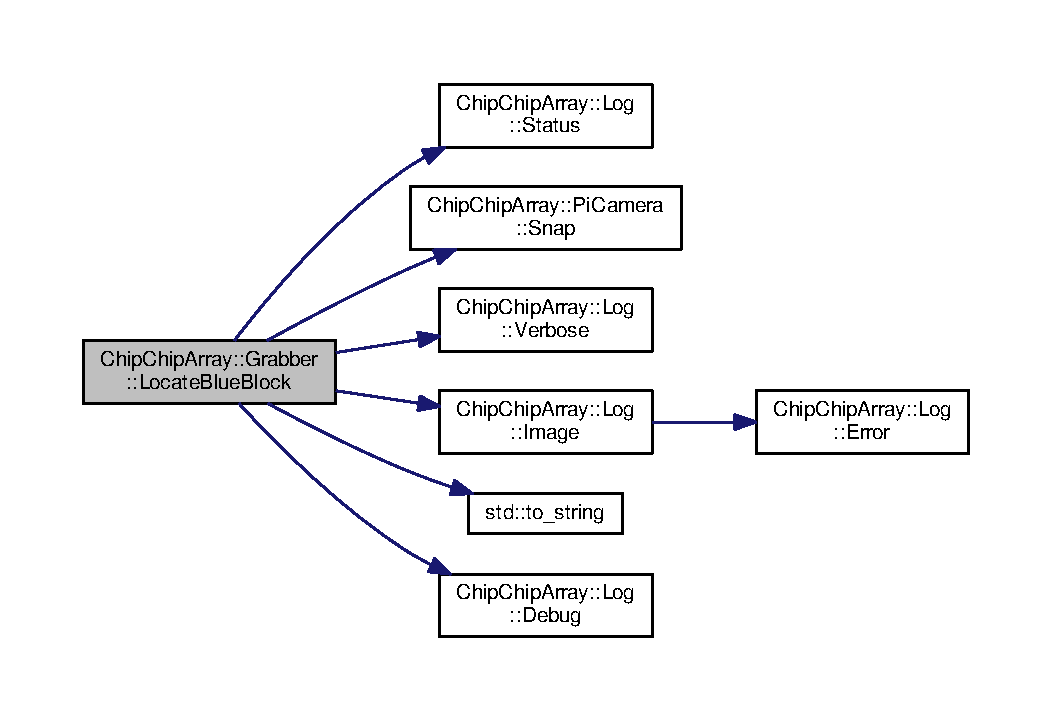
\includegraphics[width=350pt]{classChipChipArray_1_1Grabber_ab9b0d6a64b2c94c0d0f810a5ebeef6ec_cgraph}
\end{center}
\end{figure}




Here is the caller graph for this function\+:
\nopagebreak
\begin{figure}[H]
\begin{center}
\leavevmode
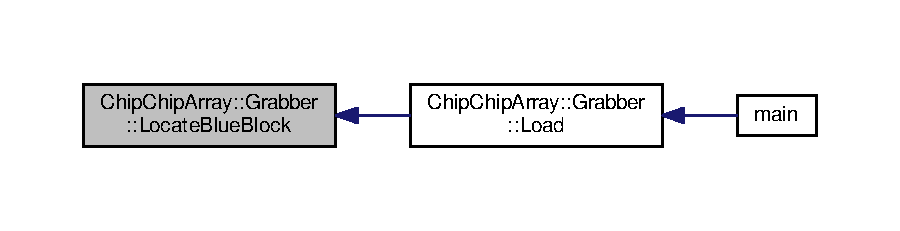
\includegraphics[width=350pt]{classChipChipArray_1_1Grabber_ab9b0d6a64b2c94c0d0f810a5ebeef6ec_icgraph}
\end{center}
\end{figure}




\subsection{Member Data Documentation}
\hypertarget{classChipChipArray_1_1Grabber_a726bcc2367a719cb84de92a981947622}{\index{Chip\+Chip\+Array\+::\+Grabber@{Chip\+Chip\+Array\+::\+Grabber}!cam@{cam}}
\index{cam@{cam}!Chip\+Chip\+Array\+::\+Grabber@{Chip\+Chip\+Array\+::\+Grabber}}
\subsubsection[{cam}]{\setlength{\rightskip}{0pt plus 5cm}{\bf Pi\+Camera} Chip\+Chip\+Array\+::\+Grabber\+::cam\hspace{0.3cm}{\ttfamily [protected]}}}\label{classChipChipArray_1_1Grabber_a726bcc2367a719cb84de92a981947622}
The Raspicam 

Definition at line \hyperlink{Grabber_8hpp_source_l00064}{64} of file \hyperlink{Grabber_8hpp_source}{Grabber.\+hpp}.

\hypertarget{classChipChipArray_1_1Grabber_a8afbaefae7c767c862fd1bf13968539b}{\index{Chip\+Chip\+Array\+::\+Grabber@{Chip\+Chip\+Array\+::\+Grabber}!side@{side}}
\index{side@{side}!Chip\+Chip\+Array\+::\+Grabber@{Chip\+Chip\+Array\+::\+Grabber}}
\subsubsection[{side}]{\setlength{\rightskip}{0pt plus 5cm}{\bf Side} Chip\+Chip\+Array\+::\+Grabber\+::side\hspace{0.3cm}{\ttfamily [protected]}}}\label{classChipChipArray_1_1Grabber_a8afbaefae7c767c862fd1bf13968539b}
The side from which the robot is coming (i.\+e., the side where the higher priority blocks are to be picked up. 

Definition at line \hyperlink{Grabber_8hpp_source_l00071}{71} of file \hyperlink{Grabber_8hpp_source}{Grabber.\+hpp}.

\hypertarget{classChipChipArray_1_1Grabber_ab57efe6e0b6f369b19528285a278d967}{\index{Chip\+Chip\+Array\+::\+Grabber@{Chip\+Chip\+Array\+::\+Grabber}!zone@{zone}}
\index{zone@{zone}!Chip\+Chip\+Array\+::\+Grabber@{Chip\+Chip\+Array\+::\+Grabber}}
\subsubsection[{zone}]{\setlength{\rightskip}{0pt plus 5cm}{\bf Zone} Chip\+Chip\+Array\+::\+Grabber\+::zone\hspace{0.3cm}{\ttfamily [protected]}}}\label{classChipChipArray_1_1Grabber_ab57efe6e0b6f369b19528285a278d967}
The zone in which blocks are being loaded. 

Definition at line \hyperlink{Grabber_8hpp_source_l00076}{76} of file \hyperlink{Grabber_8hpp_source}{Grabber.\+hpp}.



The documentation for this class was generated from the following file\+:\begin{DoxyCompactItemize}
\item 
src/\hyperlink{Grabber_8hpp}{Grabber.\+hpp}\end{DoxyCompactItemize}

\hypertarget{classChipChipArray_1_1Log}{\section{Chip\+Chip\+Array\+:\+:Log Class Reference}
\label{classChipChipArray_1_1Log}\index{Chip\+Chip\+Array\+::\+Log@{Chip\+Chip\+Array\+::\+Log}}
}


{\ttfamily \#include $<$Log.\+hpp$>$}

\subsection*{Public Member Functions}
\begin{DoxyCompactItemize}
\item 
\hyperlink{classChipChipArray_1_1Log_a2bd48afdb832567e94545e6dc2f6f4d5}{Log} ()
\item 
\hyperlink{classChipChipArray_1_1Log_a4cd28a821789b39e936a6e346329d65b}{Log} (auto dir, \hyperlink{definitions_8hpp_aa7380b6d694cab49f07aed6a7af592d9}{Log\+Mode} mode=\hyperlink{definitions_8hpp_aa7380b6d694cab49f07aed6a7af592d9a9dffbf69ffba8bc38bc4e01abf4b1675}{Log\+Mode\+::\+Text})
\item 
\hyperlink{classChipChipArray_1_1Log_a647df4da22b29d9d5a5ea32af3a1ed83}{$\sim$\+Log} ()
\item 
void \hyperlink{classChipChipArray_1_1Log_ac32b435af1577e4ebc67af2bdfea8eff}{Debug} (auto mesg)
\item 
void \hyperlink{classChipChipArray_1_1Log_aba7b7b0555f49f4dcf15f4b9fd3e6b34}{Error} (auto mesg)
\item 
void \hyperlink{classChipChipArray_1_1Log_a65bbab057c8b1453f9e4efcfee7522c4}{Image} (cv\+::\+Mat image, auto filename)
\item 
void \hyperlink{classChipChipArray_1_1Log_ad27a06a4561f2f59159bd8a7fc2fed3b}{Open} (auto dir, \hyperlink{definitions_8hpp_aa7380b6d694cab49f07aed6a7af592d9}{Log\+Mode} mode=\hyperlink{definitions_8hpp_aa7380b6d694cab49f07aed6a7af592d9a9dffbf69ffba8bc38bc4e01abf4b1675}{Log\+Mode\+::\+Text})
\item 
void \hyperlink{classChipChipArray_1_1Log_a66575b6e94c6112e4cefa5736cb996e0}{Status} (auto mesg)
\item 
void \hyperlink{classChipChipArray_1_1Log_a8849569720c26e335e7ef4dcb912170b}{Variable} (auto name, auto value)
\item 
void \hyperlink{classChipChipArray_1_1Log_a154a5f38d9c7a767693b242684a3d4d9}{Verbose} (auto mesg)
\end{DoxyCompactItemize}


\subsection{Detailed Description}
This class logs the text and images passed to it to specificed directory.

A \char`\"{}container\char`\"{} directory to which the class can write is passed in the constructor. When the \hyperlink{classChipChipArray_1_1Log}{Log} is initialized with \hyperlink{definitions_8hpp_aa7380b6d694cab49f07aed6a7af592d9a9dffbf69ffba8bc38bc4e01abf4b1675}{Log\+Mode\+::\+Text}, a new log file is created with a filename based on the time of initialization in the given directory. When initialized in \hyperlink{definitions_8hpp_aa7380b6d694cab49f07aed6a7af592d9ace7898536dd0e928d1640ee2ad531cc8}{Log\+Mode\+::\+Multi}, it will create a subdirectory in the given directory with a name based on time. In this new directory, a log file will be created. Images may later be stored in this directory with names based on the order in which they were saved.

This class D\+O\+E\+S N\+O\+T W\+O\+R\+K without compiling without a \char`\"{}\+L\+O\+G\char`\"{} definition (\#define L\+O\+G or -\/\+D\+L\+O\+G). 

Definition at line 34 of file Log.\+hpp.



\subsection{Constructor \& Destructor Documentation}
\hypertarget{classChipChipArray_1_1Log_a2bd48afdb832567e94545e6dc2f6f4d5}{\index{Chip\+Chip\+Array\+::\+Log@{Chip\+Chip\+Array\+::\+Log}!Log@{Log}}
\index{Log@{Log}!Chip\+Chip\+Array\+::\+Log@{Chip\+Chip\+Array\+::\+Log}}
\subsubsection[{Log}]{\setlength{\rightskip}{0pt plus 5cm}Chip\+Chip\+Array\+::\+Log\+::\+Log (
\begin{DoxyParamCaption}
{}
\end{DoxyParamCaption}
)\hspace{0.3cm}{\ttfamily [inline]}}}\label{classChipChipArray_1_1Log_a2bd48afdb832567e94545e6dc2f6f4d5}
Initializes \hyperlink{classChipChipArray_1_1Log}{Log} object but does not open log. \hyperlink{classChipChipArray_1_1Log_ad27a06a4561f2f59159bd8a7fc2fed3b}{Open()} must be called. 

Definition at line 40 of file Log.\+hpp.

\hypertarget{classChipChipArray_1_1Log_a4cd28a821789b39e936a6e346329d65b}{\index{Chip\+Chip\+Array\+::\+Log@{Chip\+Chip\+Array\+::\+Log}!Log@{Log}}
\index{Log@{Log}!Chip\+Chip\+Array\+::\+Log@{Chip\+Chip\+Array\+::\+Log}}
\subsubsection[{Log}]{\setlength{\rightskip}{0pt plus 5cm}Chip\+Chip\+Array\+::\+Log\+::\+Log (
\begin{DoxyParamCaption}
\item[{auto}]{dir, }
\item[{{\bf Log\+Mode}}]{mode = {\ttfamily {\bf Log\+Mode\+::\+Text}}}
\end{DoxyParamCaption}
)}}\label{classChipChipArray_1_1Log_a4cd28a821789b39e936a6e346329d65b}
Initializes the \hyperlink{classChipChipArray_1_1Log}{Log}.

A new log file is created in dir if \hyperlink{definitions_8hpp_aa7380b6d694cab49f07aed6a7af592d9a9dffbf69ffba8bc38bc4e01abf4b1675}{Log\+Mode\+::\+Text} is given. The file will have a name based on the current date and time. If \hyperlink{definitions_8hpp_aa7380b6d694cab49f07aed6a7af592d9ace7898536dd0e928d1640ee2ad531cc8}{Log\+Mode\+::\+Multi} is given, a new directory is created, and a log file with a name based on the current date and time is created inside it.


\begin{DoxyParams}{Parameters}
{\em dir} & the directory for the newly created logfile/folder\\
\hline
{\em mode} & the Log\+Mode \\
\hline
\end{DoxyParams}


Definition at line 186 of file Log.\+hpp.



Here is the call graph for this function\+:
\nopagebreak
\begin{figure}[H]
\begin{center}
\leavevmode
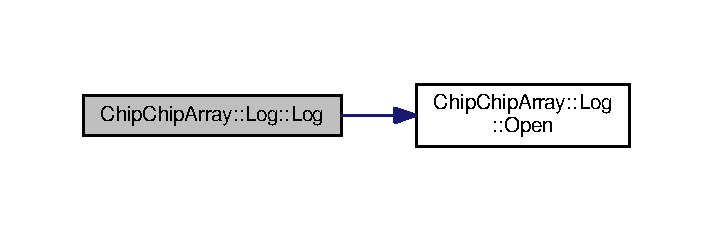
\includegraphics[width=342pt]{classChipChipArray_1_1Log_a4cd28a821789b39e936a6e346329d65b_cgraph}
\end{center}
\end{figure}


\hypertarget{classChipChipArray_1_1Log_a647df4da22b29d9d5a5ea32af3a1ed83}{\index{Chip\+Chip\+Array\+::\+Log@{Chip\+Chip\+Array\+::\+Log}!````~Log@{$\sim$\+Log}}
\index{````~Log@{$\sim$\+Log}!Chip\+Chip\+Array\+::\+Log@{Chip\+Chip\+Array\+::\+Log}}
\subsubsection[{$\sim$\+Log}]{\setlength{\rightskip}{0pt plus 5cm}Chip\+Chip\+Array\+::\+Log\+::$\sim$\+Log (
\begin{DoxyParamCaption}
{}
\end{DoxyParamCaption}
)}}\label{classChipChipArray_1_1Log_a647df4da22b29d9d5a5ea32af3a1ed83}
Destroys the \hyperlink{classChipChipArray_1_1Log}{Log} and closes the logfile. 

Definition at line 192 of file Log.\+hpp.



\subsection{Member Function Documentation}
\hypertarget{classChipChipArray_1_1Log_ac32b435af1577e4ebc67af2bdfea8eff}{\index{Chip\+Chip\+Array\+::\+Log@{Chip\+Chip\+Array\+::\+Log}!Debug@{Debug}}
\index{Debug@{Debug}!Chip\+Chip\+Array\+::\+Log@{Chip\+Chip\+Array\+::\+Log}}
\subsubsection[{Debug}]{\setlength{\rightskip}{0pt plus 5cm}void Chip\+Chip\+Array\+::\+Log\+::\+Debug (
\begin{DoxyParamCaption}
\item[{auto}]{mesg}
\end{DoxyParamCaption}
)}}\label{classChipChipArray_1_1Log_ac32b435af1577e4ebc67af2bdfea8eff}
Writes \char`\"{}\+D\+E\+B\+U\+G\+: \char`\"{} to the log file along with the message passed. Should be used for generic debugging information. If recording the value of a variable in the \hyperlink{classChipChipArray_1_1Log}{Log} is desired, use the function \hyperlink{classChipChipArray_1_1Log_a8849569720c26e335e7ef4dcb912170b}{Variable()} instead.


\begin{DoxyParams}{Parameters}
{\em mesg} & the message to record in the logfile \\
\hline
\end{DoxyParams}


Definition at line 204 of file Log.\+hpp.



Here is the caller graph for this function\+:
\nopagebreak
\begin{figure}[H]
\begin{center}
\leavevmode
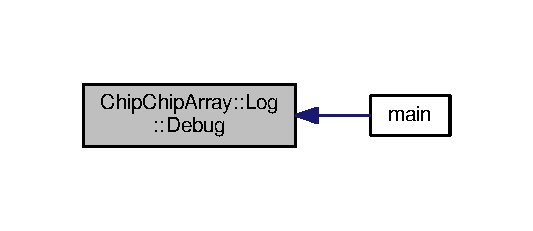
\includegraphics[width=256pt]{classChipChipArray_1_1Log_ac32b435af1577e4ebc67af2bdfea8eff_icgraph}
\end{center}
\end{figure}


\hypertarget{classChipChipArray_1_1Log_aba7b7b0555f49f4dcf15f4b9fd3e6b34}{\index{Chip\+Chip\+Array\+::\+Log@{Chip\+Chip\+Array\+::\+Log}!Error@{Error}}
\index{Error@{Error}!Chip\+Chip\+Array\+::\+Log@{Chip\+Chip\+Array\+::\+Log}}
\subsubsection[{Error}]{\setlength{\rightskip}{0pt plus 5cm}void Chip\+Chip\+Array\+::\+Log\+::\+Error (
\begin{DoxyParamCaption}
\item[{auto}]{mesg}
\end{DoxyParamCaption}
)}}\label{classChipChipArray_1_1Log_aba7b7b0555f49f4dcf15f4b9fd3e6b34}
Writes \char`\"{}\+E\+R\+R\+O\+R\+: \char`\"{} to the log file. Should only be use when an exception is thrown.


\begin{DoxyParams}{Parameters}
{\em mesg} & the message to record in the log \\
\hline
\end{DoxyParams}


Definition at line 215 of file Log.\+hpp.



Here is the caller graph for this function\+:
\nopagebreak
\begin{figure}[H]
\begin{center}
\leavevmode
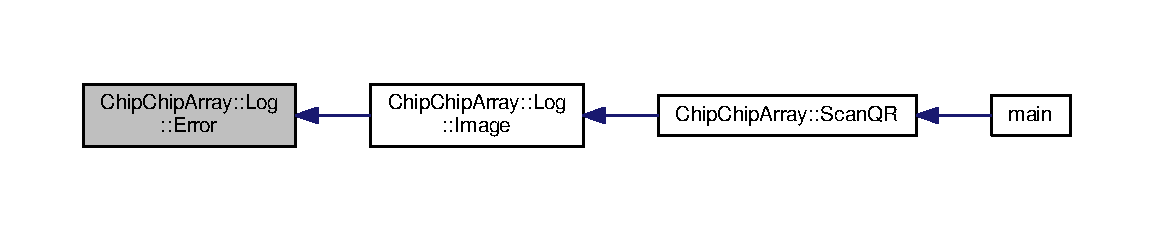
\includegraphics[width=350pt]{classChipChipArray_1_1Log_aba7b7b0555f49f4dcf15f4b9fd3e6b34_icgraph}
\end{center}
\end{figure}


\hypertarget{classChipChipArray_1_1Log_a65bbab057c8b1453f9e4efcfee7522c4}{\index{Chip\+Chip\+Array\+::\+Log@{Chip\+Chip\+Array\+::\+Log}!Image@{Image}}
\index{Image@{Image}!Chip\+Chip\+Array\+::\+Log@{Chip\+Chip\+Array\+::\+Log}}
\subsubsection[{Image}]{\setlength{\rightskip}{0pt plus 5cm}void Chip\+Chip\+Array\+::\+Log\+::\+Image (
\begin{DoxyParamCaption}
\item[{cv\+::\+Mat}]{image, }
\item[{auto}]{filename}
\end{DoxyParamCaption}
)}}\label{classChipChipArray_1_1Log_a65bbab057c8b1453f9e4efcfee7522c4}
Creates a bitmap image in the subdirectory created by the \hyperlink{classChipChipArray_1_1Log}{Log} during initialization. Does nothing if \hyperlink{definitions_8hpp_aa7380b6d694cab49f07aed6a7af592d9a9dffbf69ffba8bc38bc4e01abf4b1675}{Log\+Mode\+::\+Text} was passed in the constructor.


\begin{DoxyParams}{Parameters}
{\em image} & the image to save \\
\hline
{\em filename} & the filename for the saved image \\
\hline
\end{DoxyParams}


Definition at line 226 of file Log.\+hpp.



Here is the call graph for this function\+:
\nopagebreak
\begin{figure}[H]
\begin{center}
\leavevmode
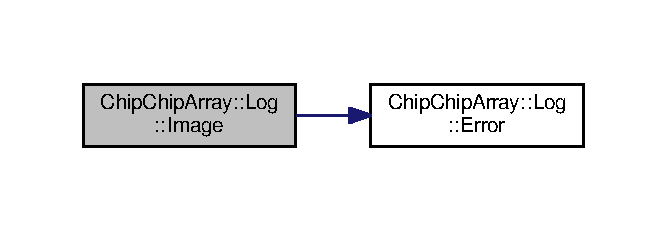
\includegraphics[width=320pt]{classChipChipArray_1_1Log_a65bbab057c8b1453f9e4efcfee7522c4_cgraph}
\end{center}
\end{figure}




Here is the caller graph for this function\+:
\nopagebreak
\begin{figure}[H]
\begin{center}
\leavevmode
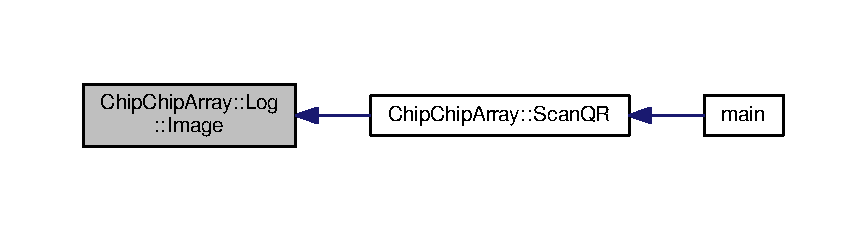
\includegraphics[width=350pt]{classChipChipArray_1_1Log_a65bbab057c8b1453f9e4efcfee7522c4_icgraph}
\end{center}
\end{figure}


\hypertarget{classChipChipArray_1_1Log_ad27a06a4561f2f59159bd8a7fc2fed3b}{\index{Chip\+Chip\+Array\+::\+Log@{Chip\+Chip\+Array\+::\+Log}!Open@{Open}}
\index{Open@{Open}!Chip\+Chip\+Array\+::\+Log@{Chip\+Chip\+Array\+::\+Log}}
\subsubsection[{Open}]{\setlength{\rightskip}{0pt plus 5cm}void Chip\+Chip\+Array\+::\+Log\+::\+Open (
\begin{DoxyParamCaption}
\item[{auto}]{dir, }
\item[{{\bf Log\+Mode}}]{mode = {\ttfamily {\bf Log\+Mode\+::\+Text}}}
\end{DoxyParamCaption}
)}}\label{classChipChipArray_1_1Log_ad27a06a4561f2f59159bd8a7fc2fed3b}


Definition at line 246 of file Log.\+hpp.



Here is the caller graph for this function\+:
\nopagebreak
\begin{figure}[H]
\begin{center}
\leavevmode
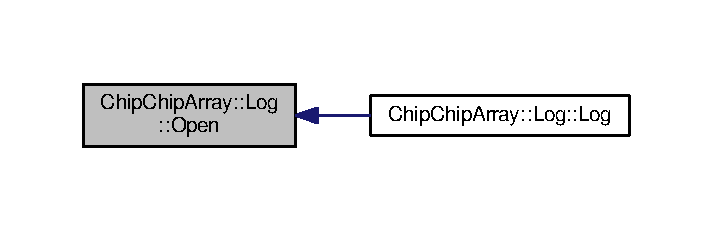
\includegraphics[width=342pt]{classChipChipArray_1_1Log_ad27a06a4561f2f59159bd8a7fc2fed3b_icgraph}
\end{center}
\end{figure}


\hypertarget{classChipChipArray_1_1Log_a66575b6e94c6112e4cefa5736cb996e0}{\index{Chip\+Chip\+Array\+::\+Log@{Chip\+Chip\+Array\+::\+Log}!Status@{Status}}
\index{Status@{Status}!Chip\+Chip\+Array\+::\+Log@{Chip\+Chip\+Array\+::\+Log}}
\subsubsection[{Status}]{\setlength{\rightskip}{0pt plus 5cm}void Chip\+Chip\+Array\+::\+Log\+::\+Status (
\begin{DoxyParamCaption}
\item[{auto}]{mesg}
\end{DoxyParamCaption}
)}}\label{classChipChipArray_1_1Log_a66575b6e94c6112e4cefa5736cb996e0}
Writes \char`\"{}\+S\+T\+A\+T\+U\+S\+: \char`\"{} to the log file. Should be used when recording the status or state of the program. It should not be used to record microalgorithmic changes. Use \hyperlink{classChipChipArray_1_1Log_a154a5f38d9c7a767693b242684a3d4d9}{Verbose()} for these instead.


\begin{DoxyParams}{Parameters}
{\em mesg} & the message to record in the logfile \\
\hline
\end{DoxyParams}


Definition at line 289 of file Log.\+hpp.



Here is the caller graph for this function\+:
\nopagebreak
\begin{figure}[H]
\begin{center}
\leavevmode
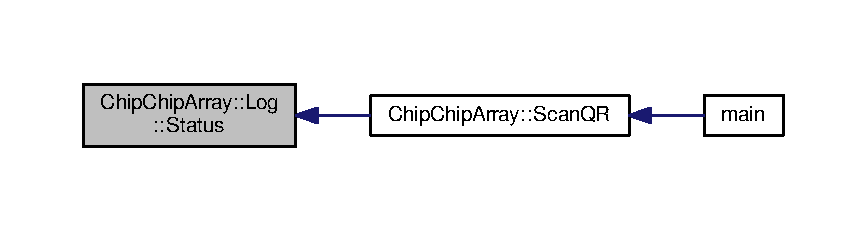
\includegraphics[width=350pt]{classChipChipArray_1_1Log_a66575b6e94c6112e4cefa5736cb996e0_icgraph}
\end{center}
\end{figure}


\hypertarget{classChipChipArray_1_1Log_a8849569720c26e335e7ef4dcb912170b}{\index{Chip\+Chip\+Array\+::\+Log@{Chip\+Chip\+Array\+::\+Log}!Variable@{Variable}}
\index{Variable@{Variable}!Chip\+Chip\+Array\+::\+Log@{Chip\+Chip\+Array\+::\+Log}}
\subsubsection[{Variable}]{\setlength{\rightskip}{0pt plus 5cm}void Chip\+Chip\+Array\+::\+Log\+::\+Variable (
\begin{DoxyParamCaption}
\item[{auto}]{name, }
\item[{auto}]{value}
\end{DoxyParamCaption}
)}}\label{classChipChipArray_1_1Log_a8849569720c26e335e7ef4dcb912170b}
Writes \char`\"{}\+V\+A\+R\+I\+A\+B\+L\+E\+: \char`\"{} to the log file. Should be used whenever recording the value of a variable is desired.


\begin{DoxyParams}{Parameters}
{\em name} & the variable name to record \\
\hline
{\em value} & the variable value to record \\
\hline
\end{DoxyParams}


Definition at line 300 of file Log.\+hpp.



Here is the caller graph for this function\+:
\nopagebreak
\begin{figure}[H]
\begin{center}
\leavevmode
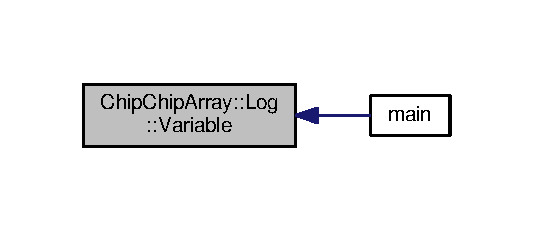
\includegraphics[width=256pt]{classChipChipArray_1_1Log_a8849569720c26e335e7ef4dcb912170b_icgraph}
\end{center}
\end{figure}


\hypertarget{classChipChipArray_1_1Log_a154a5f38d9c7a767693b242684a3d4d9}{\index{Chip\+Chip\+Array\+::\+Log@{Chip\+Chip\+Array\+::\+Log}!Verbose@{Verbose}}
\index{Verbose@{Verbose}!Chip\+Chip\+Array\+::\+Log@{Chip\+Chip\+Array\+::\+Log}}
\subsubsection[{Verbose}]{\setlength{\rightskip}{0pt plus 5cm}void Chip\+Chip\+Array\+::\+Log\+::\+Verbose (
\begin{DoxyParamCaption}
\item[{auto}]{mesg}
\end{DoxyParamCaption}
)}}\label{classChipChipArray_1_1Log_a154a5f38d9c7a767693b242684a3d4d9}
Writes \char`\"{}\+V\+E\+R\+B\+O\+S\+E\+: \char`\"{} to the log file. Should only be used for recording small, specific portions of code. To record a change in the more general state of the program, use \hyperlink{classChipChipArray_1_1Log_a66575b6e94c6112e4cefa5736cb996e0}{Status()} instead.


\begin{DoxyParams}{Parameters}
{\em mesg} & the message to record in the logfile \\
\hline
\end{DoxyParams}


Definition at line 312 of file Log.\+hpp.



Here is the caller graph for this function\+:
\nopagebreak
\begin{figure}[H]
\begin{center}
\leavevmode
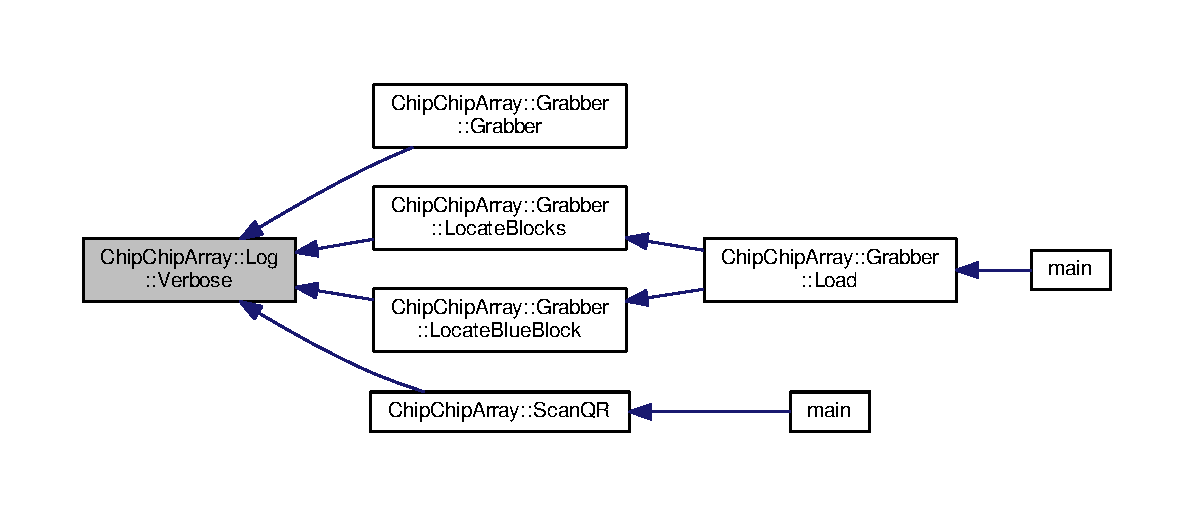
\includegraphics[width=350pt]{classChipChipArray_1_1Log_a154a5f38d9c7a767693b242684a3d4d9_icgraph}
\end{center}
\end{figure}




The documentation for this class was generated from the following file\+:\begin{DoxyCompactItemize}
\item 
src/\hyperlink{Log_8hpp}{Log.\+hpp}\end{DoxyCompactItemize}

\hypertarget{classChipChipArray_1_1PiCamera}{\section{Chip\+Chip\+Array\+:\+:Pi\+Camera Class Reference}
\label{classChipChipArray_1_1PiCamera}\index{Chip\+Chip\+Array\+::\+Pi\+Camera@{Chip\+Chip\+Array\+::\+Pi\+Camera}}
}


{\ttfamily \#include $<$Pi\+Camera.\+hpp$>$}

\subsection*{Public Member Functions}
\begin{DoxyCompactItemize}
\item 
\hyperlink{classChipChipArray_1_1PiCamera_a5910a3284877677decb6529d88e43487}{Pi\+Camera} ()
\item 
\hyperlink{classChipChipArray_1_1PiCamera_a0a4480e9e7475ae7af9a7523239caf8d}{Pi\+Camera} (bool use\+Color)
\item 
void \hyperlink{classChipChipArray_1_1PiCamera_a38f8205921d6deec5a2c360ea7d24cc5}{Close} ()
\item 
cv\+::\+Mat \hyperlink{classChipChipArray_1_1PiCamera_a58fb0de02570dce9a9cb60a1a04fb84f}{Snap} ()
\end{DoxyCompactItemize}


\subsection{Detailed Description}
This class is a basic wrapper to allow the Raspicam to interface with Open\+C\+V. It uses another wrapper class, Raspicam, provided by Cédric Verstraeten (\href{https://github.com/cedricve/raspicam}{\tt https\+://github.\+com/cedricve/raspicam}). 

Definition at line \hyperlink{PiCamera_8hpp_source_l00024}{24} of file \hyperlink{PiCamera_8hpp_source}{Pi\+Camera.\+hpp}.



\subsection{Constructor \& Destructor Documentation}
\hypertarget{classChipChipArray_1_1PiCamera_a5910a3284877677decb6529d88e43487}{\index{Chip\+Chip\+Array\+::\+Pi\+Camera@{Chip\+Chip\+Array\+::\+Pi\+Camera}!Pi\+Camera@{Pi\+Camera}}
\index{Pi\+Camera@{Pi\+Camera}!Chip\+Chip\+Array\+::\+Pi\+Camera@{Chip\+Chip\+Array\+::\+Pi\+Camera}}
\subsubsection[{Pi\+Camera}]{\setlength{\rightskip}{0pt plus 5cm}Chip\+Chip\+Array\+::\+Pi\+Camera\+::\+Pi\+Camera (
\begin{DoxyParamCaption}
{}
\end{DoxyParamCaption}
)\hspace{0.3cm}{\ttfamily [inline]}}}\label{classChipChipArray_1_1PiCamera_a5910a3284877677decb6529d88e43487}
Opens the camera and configures it for color images. 

Definition at line \hyperlink{PiCamera_8hpp_source_l00029}{29} of file \hyperlink{PiCamera_8hpp_source}{Pi\+Camera.\+hpp}.


\begin{DoxyCode}
00029 : \hyperlink{classChipChipArray_1_1PiCamera_a5910a3284877677decb6529d88e43487}{PiCamera}(\textcolor{keyword}{true}) \{\};
\end{DoxyCode}
\hypertarget{classChipChipArray_1_1PiCamera_a0a4480e9e7475ae7af9a7523239caf8d}{\index{Chip\+Chip\+Array\+::\+Pi\+Camera@{Chip\+Chip\+Array\+::\+Pi\+Camera}!Pi\+Camera@{Pi\+Camera}}
\index{Pi\+Camera@{Pi\+Camera}!Chip\+Chip\+Array\+::\+Pi\+Camera@{Chip\+Chip\+Array\+::\+Pi\+Camera}}
\subsubsection[{Pi\+Camera}]{\setlength{\rightskip}{0pt plus 5cm}Chip\+Chip\+Array\+::\+Pi\+Camera\+::\+Pi\+Camera (
\begin{DoxyParamCaption}
\item[{bool}]{use\+Color}
\end{DoxyParamCaption}
)}}\label{classChipChipArray_1_1PiCamera_a0a4480e9e7475ae7af9a7523239caf8d}
Opens the camera.


\begin{DoxyParams}{Parameters}
{\em use\+Color} & Specifices whether camera should make color images. T\+R\+U\+E = color, F\+A\+L\+S\+E = grayscale. \\
\hline
\end{DoxyParams}


Definition at line \hyperlink{PiCamera_8hpp_source_l00059}{59} of file \hyperlink{PiCamera_8hpp_source}{Pi\+Camera.\+hpp}.


\begin{DoxyCode}
00059                                     \{
00060         cam.set(CV\_CAP\_PROP\_FORMAT, (useColor ? CV\_16UC3 : CV\_16UC1));
00061         cam.open();
00062         usleep(500000);  \textcolor{comment}{// required to allow camera time to adjust!}
00063     \}
\end{DoxyCode}


\subsection{Member Function Documentation}
\hypertarget{classChipChipArray_1_1PiCamera_a38f8205921d6deec5a2c360ea7d24cc5}{\index{Chip\+Chip\+Array\+::\+Pi\+Camera@{Chip\+Chip\+Array\+::\+Pi\+Camera}!Close@{Close}}
\index{Close@{Close}!Chip\+Chip\+Array\+::\+Pi\+Camera@{Chip\+Chip\+Array\+::\+Pi\+Camera}}
\subsubsection[{Close}]{\setlength{\rightskip}{0pt plus 5cm}void Chip\+Chip\+Array\+::\+Pi\+Camera\+::\+Close (
\begin{DoxyParamCaption}
{}
\end{DoxyParamCaption}
)}}\label{classChipChipArray_1_1PiCamera_a38f8205921d6deec5a2c360ea7d24cc5}
Closes connection to camera. 

Definition at line \hyperlink{PiCamera_8hpp_source_l00065}{65} of file \hyperlink{PiCamera_8hpp_source}{Pi\+Camera.\+hpp}.


\begin{DoxyCode}
00065                          \{
00066         cam.release();
00067     \}
\end{DoxyCode}


Here is the caller graph for this function\+:
\nopagebreak
\begin{figure}[H]
\begin{center}
\leavevmode
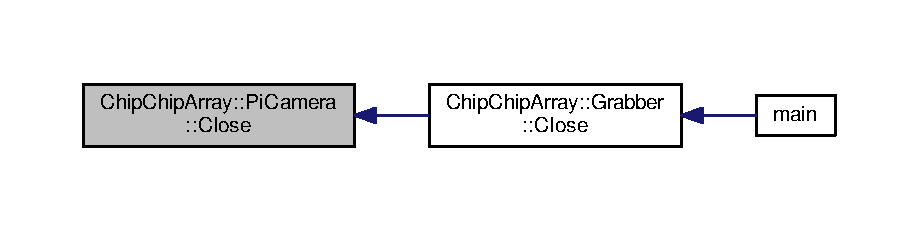
\includegraphics[width=350pt]{classChipChipArray_1_1PiCamera_a38f8205921d6deec5a2c360ea7d24cc5_icgraph}
\end{center}
\end{figure}


\hypertarget{classChipChipArray_1_1PiCamera_a58fb0de02570dce9a9cb60a1a04fb84f}{\index{Chip\+Chip\+Array\+::\+Pi\+Camera@{Chip\+Chip\+Array\+::\+Pi\+Camera}!Snap@{Snap}}
\index{Snap@{Snap}!Chip\+Chip\+Array\+::\+Pi\+Camera@{Chip\+Chip\+Array\+::\+Pi\+Camera}}
\subsubsection[{Snap}]{\setlength{\rightskip}{0pt plus 5cm}cv\+::\+Mat Chip\+Chip\+Array\+::\+Pi\+Camera\+::\+Snap (
\begin{DoxyParamCaption}
{}
\end{DoxyParamCaption}
)}}\label{classChipChipArray_1_1PiCamera_a58fb0de02570dce9a9cb60a1a04fb84f}
Makes picture.

\begin{DoxyReturn}{Returns}
Open\+C\+V Mat object (i.\+e., an image) from the camera 
\end{DoxyReturn}


Definition at line \hyperlink{PiCamera_8hpp_source_l00069}{69} of file \hyperlink{PiCamera_8hpp_source}{Pi\+Camera.\+hpp}.


\begin{DoxyCode}
00069                          \{
00070         \textcolor{keywordflow}{if}(!cam.isOpened()) \textcolor{keywordflow}{throw} std::runtime\_error(\textcolor{stringliteral}{"Camera "}
00071                 \textcolor{stringliteral}{"is not open!"});
00072 
00073         cv::Mat image;
00074         cam.grab();
00075         cam.retrieve(image);
00076         \textcolor{keywordflow}{return} image;
00077     \}
\end{DoxyCode}


Here is the caller graph for this function\+:
\nopagebreak
\begin{figure}[H]
\begin{center}
\leavevmode
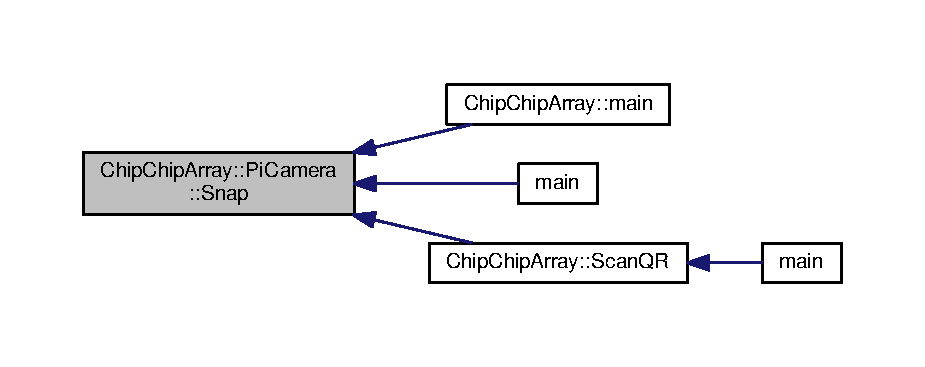
\includegraphics[width=350pt]{classChipChipArray_1_1PiCamera_a58fb0de02570dce9a9cb60a1a04fb84f_icgraph}
\end{center}
\end{figure}




The documentation for this class was generated from the following file\+:\begin{DoxyCompactItemize}
\item 
src/\hyperlink{PiCamera_8hpp}{Pi\+Camera.\+hpp}\end{DoxyCompactItemize}

\chapter{File Documentation}
\hypertarget{doxygen_8config}{\section{etc/doxygen.config File Reference}
\label{doxygen_8config}\index{etc/doxygen.\+config@{etc/doxygen.\+config}}
}

\hypertarget{makefile}{\section{makefile File Reference}
\label{makefile}\index{makefile@{makefile}}
}

\hypertarget{Adafruit__PWMServoDriver_8cpp}{\section{src/\+Adafruit\+\_\+\+P\+W\+M\+Servo\+Driver.cpp File Reference}
\label{Adafruit__PWMServoDriver_8cpp}\index{src/\+Adafruit\+\_\+\+P\+W\+M\+Servo\+Driver.\+cpp@{src/\+Adafruit\+\_\+\+P\+W\+M\+Servo\+Driver.\+cpp}}
}
{\ttfamily \#include \char`\"{}Adafruit\+\_\+\+P\+W\+M\+Servo\+Driver.\+h\char`\"{}}\\*
Include dependency graph for Adafruit\+\_\+\+P\+W\+M\+Servo\+Driver.\+cpp\+:
\nopagebreak
\begin{figure}[H]
\begin{center}
\leavevmode
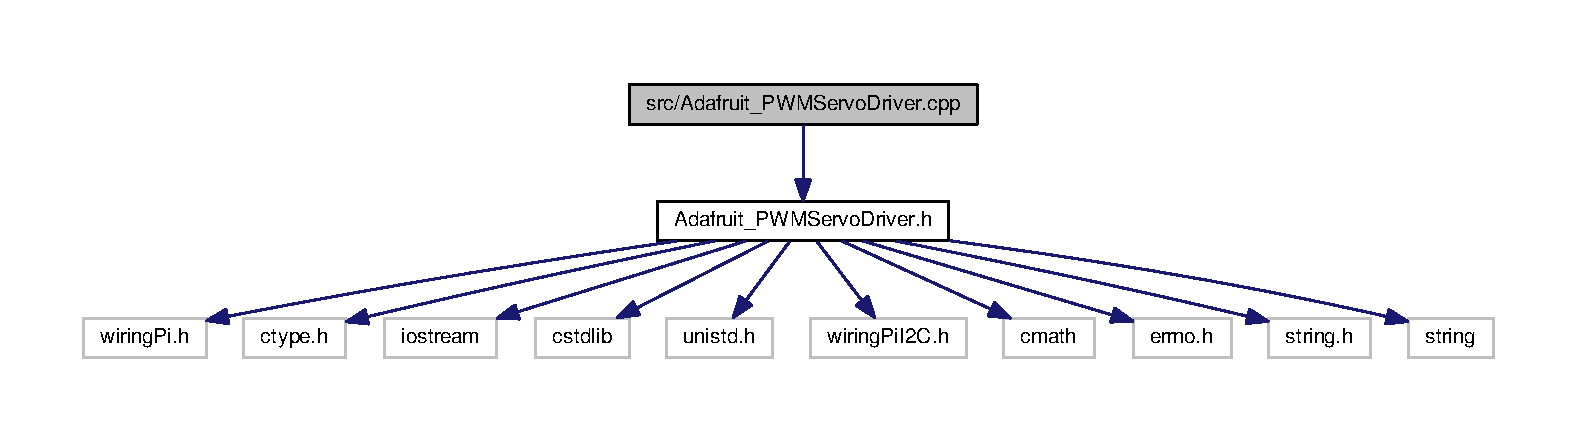
\includegraphics[width=350pt]{Adafruit__PWMServoDriver_8cpp__incl}
\end{center}
\end{figure}
This graph shows which files directly or indirectly include this file\+:
\nopagebreak
\begin{figure}[H]
\begin{center}
\leavevmode
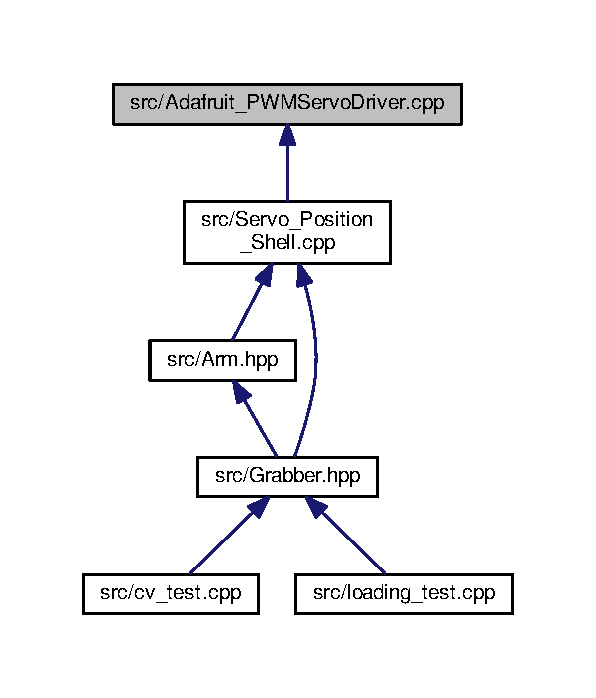
\includegraphics[width=333pt]{Adafruit__PWMServoDriver_8cpp__dep__incl}
\end{center}
\end{figure}
\subsection*{Macros}
\begin{DoxyCompactItemize}
\item 
\#define \hyperlink{Adafruit__PWMServoDriver_8cpp_a818989cbf7f37dae193fbb28b2d3976a}{E\+N\+A\+B\+L\+E\+\_\+\+D\+E\+B\+U\+G\+\_\+\+O\+U\+T\+P\+U\+T}~false
\end{DoxyCompactItemize}


\subsection{Macro Definition Documentation}
\hypertarget{Adafruit__PWMServoDriver_8cpp_a818989cbf7f37dae193fbb28b2d3976a}{\index{Adafruit\+\_\+\+P\+W\+M\+Servo\+Driver.\+cpp@{Adafruit\+\_\+\+P\+W\+M\+Servo\+Driver.\+cpp}!E\+N\+A\+B\+L\+E\+\_\+\+D\+E\+B\+U\+G\+\_\+\+O\+U\+T\+P\+U\+T@{E\+N\+A\+B\+L\+E\+\_\+\+D\+E\+B\+U\+G\+\_\+\+O\+U\+T\+P\+U\+T}}
\index{E\+N\+A\+B\+L\+E\+\_\+\+D\+E\+B\+U\+G\+\_\+\+O\+U\+T\+P\+U\+T@{E\+N\+A\+B\+L\+E\+\_\+\+D\+E\+B\+U\+G\+\_\+\+O\+U\+T\+P\+U\+T}!Adafruit\+\_\+\+P\+W\+M\+Servo\+Driver.\+cpp@{Adafruit\+\_\+\+P\+W\+M\+Servo\+Driver.\+cpp}}
\subsubsection[{E\+N\+A\+B\+L\+E\+\_\+\+D\+E\+B\+U\+G\+\_\+\+O\+U\+T\+P\+U\+T}]{\setlength{\rightskip}{0pt plus 5cm}\#define E\+N\+A\+B\+L\+E\+\_\+\+D\+E\+B\+U\+G\+\_\+\+O\+U\+T\+P\+U\+T~false}}\label{Adafruit__PWMServoDriver_8cpp_a818989cbf7f37dae193fbb28b2d3976a}


Definition at line 27 of file Adafruit\+\_\+\+P\+W\+M\+Servo\+Driver.\+cpp.


\hypertarget{Adafruit__PWMServoDriver_8h}{\section{src/\+Adafruit\+\_\+\+P\+W\+M\+Servo\+Driver.h File Reference}
\label{Adafruit__PWMServoDriver_8h}\index{src/\+Adafruit\+\_\+\+P\+W\+M\+Servo\+Driver.\+h@{src/\+Adafruit\+\_\+\+P\+W\+M\+Servo\+Driver.\+h}}
}
{\ttfamily \#include $<$wiring\+Pi.\+h$>$}\\*
{\ttfamily \#include $<$ctype.\+h$>$}\\*
{\ttfamily \#include $<$iostream$>$}\\*
{\ttfamily \#include $<$cstdlib$>$}\\*
{\ttfamily \#include $<$unistd.\+h$>$}\\*
{\ttfamily \#include $<$wiring\+Pi\+I2\+C.\+h$>$}\\*
{\ttfamily \#include $<$cmath$>$}\\*
{\ttfamily \#include $<$errno.\+h$>$}\\*
{\ttfamily \#include $<$string.\+h$>$}\\*
{\ttfamily \#include $<$string$>$}\\*
Include dependency graph for Adafruit\+\_\+\+P\+W\+M\+Servo\+Driver.\+h\+:
\nopagebreak
\begin{figure}[H]
\begin{center}
\leavevmode
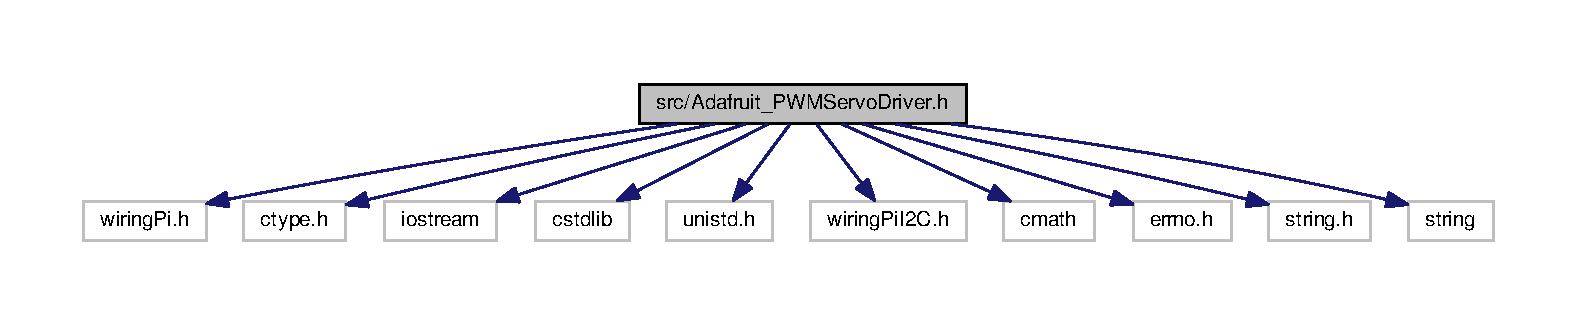
\includegraphics[width=350pt]{Adafruit__PWMServoDriver_8h__incl}
\end{center}
\end{figure}
This graph shows which files directly or indirectly include this file\+:
\nopagebreak
\begin{figure}[H]
\begin{center}
\leavevmode
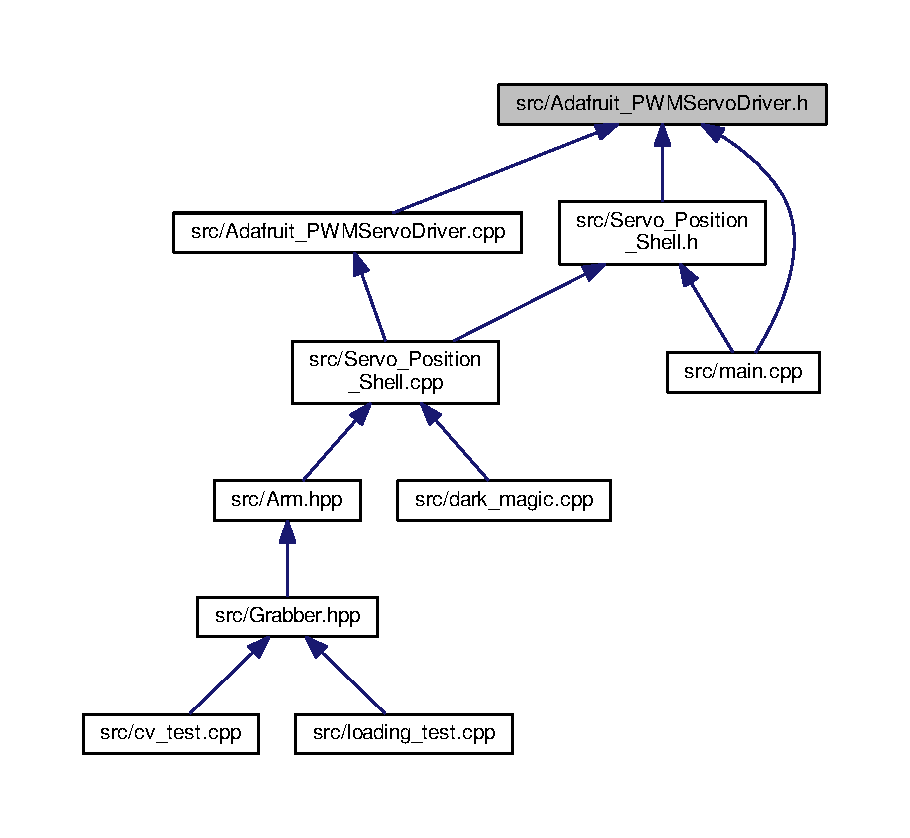
\includegraphics[width=350pt]{Adafruit__PWMServoDriver_8h__dep__incl}
\end{center}
\end{figure}
\subsection*{Classes}
\begin{DoxyCompactItemize}
\item 
class \hyperlink{classAdafruit__PWMServoDriver}{Adafruit\+\_\+\+P\+W\+M\+Servo\+Driver}
\end{DoxyCompactItemize}
\subsection*{Macros}
\begin{DoxyCompactItemize}
\item 
\#define \hyperlink{Adafruit__PWMServoDriver_8h_ad58a880e68f5aa69092c658a86641a8e}{P\+C\+A9685\+\_\+\+S\+U\+B\+A\+D\+R1}~0x2
\item 
\#define \hyperlink{Adafruit__PWMServoDriver_8h_a845ec28ef89ed81642ea5f41691d4b51}{P\+C\+A9685\+\_\+\+S\+U\+B\+A\+D\+R2}~0x3
\item 
\#define \hyperlink{Adafruit__PWMServoDriver_8h_a7f60829a2cf850c02403f5c7193b0f00}{P\+C\+A9685\+\_\+\+S\+U\+B\+A\+D\+R3}~0x4
\item 
\#define \hyperlink{Adafruit__PWMServoDriver_8h_aec642e3f25e7f83072d68acb14ae4e74}{P\+C\+A9685\+\_\+\+M\+O\+D\+E1}~0x0
\item 
\#define \hyperlink{Adafruit__PWMServoDriver_8h_a7175106bbec978d9acc85dc7485235a3}{P\+C\+A9685\+\_\+\+P\+R\+E\+S\+C\+A\+L\+E}~0x\+F\+E
\item 
\#define \hyperlink{Adafruit__PWMServoDriver_8h_a62f7dbcbb1fcf1084804f19a5b42248f}{L\+E\+D0\+\_\+\+O\+N\+\_\+\+L}~0x6
\item 
\#define \hyperlink{Adafruit__PWMServoDriver_8h_a03deab303c78b50c629847b9e0de106b}{L\+E\+D0\+\_\+\+O\+N\+\_\+\+H}~0x7
\item 
\#define \hyperlink{Adafruit__PWMServoDriver_8h_a00e3f4b43121817be365b2f22e8bad84}{L\+E\+D0\+\_\+\+O\+F\+F\+\_\+\+L}~0x8
\item 
\#define \hyperlink{Adafruit__PWMServoDriver_8h_a6d8ff6441f8d2a4fb7b4afd36b8fd329}{L\+E\+D0\+\_\+\+O\+F\+F\+\_\+\+H}~0x9
\item 
\#define \hyperlink{Adafruit__PWMServoDriver_8h_acc163ea7453bc87b5934e8b2bc838556}{A\+L\+L\+L\+E\+D\+\_\+\+O\+N\+\_\+\+L}~0x\+F\+A
\item 
\#define \hyperlink{Adafruit__PWMServoDriver_8h_a470526d36c4db534d04ec1452ddde736}{A\+L\+L\+L\+E\+D\+\_\+\+O\+N\+\_\+\+H}~0x\+F\+B
\item 
\#define \hyperlink{Adafruit__PWMServoDriver_8h_a6dc494d4156968e9cd24f7ac07bf2ee3}{A\+L\+L\+L\+E\+D\+\_\+\+O\+F\+F\+\_\+\+L}~0x\+F\+C
\item 
\#define \hyperlink{Adafruit__PWMServoDriver_8h_a11632001b28c990e5f6dee015e945b1d}{A\+L\+L\+L\+E\+D\+\_\+\+O\+F\+F\+\_\+\+H}~0x\+F\+D
\item 
\#define \hyperlink{Adafruit__PWMServoDriver_8h_ab077fa1127453be2bd9d4c3c8a768fa7}{uint8\+\_\+t}~unsigned char
\item 
\#define \hyperlink{Adafruit__PWMServoDriver_8h_a395b3b2bf5cb4674ab41b6bda68c15bb}{uint16\+\_\+t}~unsigned short int
\end{DoxyCompactItemize}


\subsection{Detailed Description}
\begin{DoxyAuthor}{Author}
Limor Fried/\+Ladyada 

Nickolas Neely  Contains the function and class headers necessary for the P\+W\+M servo driver. 
\end{DoxyAuthor}


Definition in file \hyperlink{Adafruit__PWMServoDriver_8h_source}{Adafruit\+\_\+\+P\+W\+M\+Servo\+Driver.\+h}.



\subsection{Macro Definition Documentation}
\hypertarget{Adafruit__PWMServoDriver_8h_a11632001b28c990e5f6dee015e945b1d}{\index{Adafruit\+\_\+\+P\+W\+M\+Servo\+Driver.\+h@{Adafruit\+\_\+\+P\+W\+M\+Servo\+Driver.\+h}!A\+L\+L\+L\+E\+D\+\_\+\+O\+F\+F\+\_\+\+H@{A\+L\+L\+L\+E\+D\+\_\+\+O\+F\+F\+\_\+\+H}}
\index{A\+L\+L\+L\+E\+D\+\_\+\+O\+F\+F\+\_\+\+H@{A\+L\+L\+L\+E\+D\+\_\+\+O\+F\+F\+\_\+\+H}!Adafruit\+\_\+\+P\+W\+M\+Servo\+Driver.\+h@{Adafruit\+\_\+\+P\+W\+M\+Servo\+Driver.\+h}}
\subsubsection[{A\+L\+L\+L\+E\+D\+\_\+\+O\+F\+F\+\_\+\+H}]{\setlength{\rightskip}{0pt plus 5cm}\#define A\+L\+L\+L\+E\+D\+\_\+\+O\+F\+F\+\_\+\+H~0x\+F\+D}}\label{Adafruit__PWMServoDriver_8h_a11632001b28c990e5f6dee015e945b1d}


Definition at line \hyperlink{Adafruit__PWMServoDriver_8h_source_l00062}{62} of file \hyperlink{Adafruit__PWMServoDriver_8h_source}{Adafruit\+\_\+\+P\+W\+M\+Servo\+Driver.\+h}.

\hypertarget{Adafruit__PWMServoDriver_8h_a6dc494d4156968e9cd24f7ac07bf2ee3}{\index{Adafruit\+\_\+\+P\+W\+M\+Servo\+Driver.\+h@{Adafruit\+\_\+\+P\+W\+M\+Servo\+Driver.\+h}!A\+L\+L\+L\+E\+D\+\_\+\+O\+F\+F\+\_\+\+L@{A\+L\+L\+L\+E\+D\+\_\+\+O\+F\+F\+\_\+\+L}}
\index{A\+L\+L\+L\+E\+D\+\_\+\+O\+F\+F\+\_\+\+L@{A\+L\+L\+L\+E\+D\+\_\+\+O\+F\+F\+\_\+\+L}!Adafruit\+\_\+\+P\+W\+M\+Servo\+Driver.\+h@{Adafruit\+\_\+\+P\+W\+M\+Servo\+Driver.\+h}}
\subsubsection[{A\+L\+L\+L\+E\+D\+\_\+\+O\+F\+F\+\_\+\+L}]{\setlength{\rightskip}{0pt plus 5cm}\#define A\+L\+L\+L\+E\+D\+\_\+\+O\+F\+F\+\_\+\+L~0x\+F\+C}}\label{Adafruit__PWMServoDriver_8h_a6dc494d4156968e9cd24f7ac07bf2ee3}


Definition at line \hyperlink{Adafruit__PWMServoDriver_8h_source_l00061}{61} of file \hyperlink{Adafruit__PWMServoDriver_8h_source}{Adafruit\+\_\+\+P\+W\+M\+Servo\+Driver.\+h}.

\hypertarget{Adafruit__PWMServoDriver_8h_a470526d36c4db534d04ec1452ddde736}{\index{Adafruit\+\_\+\+P\+W\+M\+Servo\+Driver.\+h@{Adafruit\+\_\+\+P\+W\+M\+Servo\+Driver.\+h}!A\+L\+L\+L\+E\+D\+\_\+\+O\+N\+\_\+\+H@{A\+L\+L\+L\+E\+D\+\_\+\+O\+N\+\_\+\+H}}
\index{A\+L\+L\+L\+E\+D\+\_\+\+O\+N\+\_\+\+H@{A\+L\+L\+L\+E\+D\+\_\+\+O\+N\+\_\+\+H}!Adafruit\+\_\+\+P\+W\+M\+Servo\+Driver.\+h@{Adafruit\+\_\+\+P\+W\+M\+Servo\+Driver.\+h}}
\subsubsection[{A\+L\+L\+L\+E\+D\+\_\+\+O\+N\+\_\+\+H}]{\setlength{\rightskip}{0pt plus 5cm}\#define A\+L\+L\+L\+E\+D\+\_\+\+O\+N\+\_\+\+H~0x\+F\+B}}\label{Adafruit__PWMServoDriver_8h_a470526d36c4db534d04ec1452ddde736}


Definition at line \hyperlink{Adafruit__PWMServoDriver_8h_source_l00060}{60} of file \hyperlink{Adafruit__PWMServoDriver_8h_source}{Adafruit\+\_\+\+P\+W\+M\+Servo\+Driver.\+h}.

\hypertarget{Adafruit__PWMServoDriver_8h_acc163ea7453bc87b5934e8b2bc838556}{\index{Adafruit\+\_\+\+P\+W\+M\+Servo\+Driver.\+h@{Adafruit\+\_\+\+P\+W\+M\+Servo\+Driver.\+h}!A\+L\+L\+L\+E\+D\+\_\+\+O\+N\+\_\+\+L@{A\+L\+L\+L\+E\+D\+\_\+\+O\+N\+\_\+\+L}}
\index{A\+L\+L\+L\+E\+D\+\_\+\+O\+N\+\_\+\+L@{A\+L\+L\+L\+E\+D\+\_\+\+O\+N\+\_\+\+L}!Adafruit\+\_\+\+P\+W\+M\+Servo\+Driver.\+h@{Adafruit\+\_\+\+P\+W\+M\+Servo\+Driver.\+h}}
\subsubsection[{A\+L\+L\+L\+E\+D\+\_\+\+O\+N\+\_\+\+L}]{\setlength{\rightskip}{0pt plus 5cm}\#define A\+L\+L\+L\+E\+D\+\_\+\+O\+N\+\_\+\+L~0x\+F\+A}}\label{Adafruit__PWMServoDriver_8h_acc163ea7453bc87b5934e8b2bc838556}


Definition at line \hyperlink{Adafruit__PWMServoDriver_8h_source_l00059}{59} of file \hyperlink{Adafruit__PWMServoDriver_8h_source}{Adafruit\+\_\+\+P\+W\+M\+Servo\+Driver.\+h}.

\hypertarget{Adafruit__PWMServoDriver_8h_a6d8ff6441f8d2a4fb7b4afd36b8fd329}{\index{Adafruit\+\_\+\+P\+W\+M\+Servo\+Driver.\+h@{Adafruit\+\_\+\+P\+W\+M\+Servo\+Driver.\+h}!L\+E\+D0\+\_\+\+O\+F\+F\+\_\+\+H@{L\+E\+D0\+\_\+\+O\+F\+F\+\_\+\+H}}
\index{L\+E\+D0\+\_\+\+O\+F\+F\+\_\+\+H@{L\+E\+D0\+\_\+\+O\+F\+F\+\_\+\+H}!Adafruit\+\_\+\+P\+W\+M\+Servo\+Driver.\+h@{Adafruit\+\_\+\+P\+W\+M\+Servo\+Driver.\+h}}
\subsubsection[{L\+E\+D0\+\_\+\+O\+F\+F\+\_\+\+H}]{\setlength{\rightskip}{0pt plus 5cm}\#define L\+E\+D0\+\_\+\+O\+F\+F\+\_\+\+H~0x9}}\label{Adafruit__PWMServoDriver_8h_a6d8ff6441f8d2a4fb7b4afd36b8fd329}


Definition at line \hyperlink{Adafruit__PWMServoDriver_8h_source_l00057}{57} of file \hyperlink{Adafruit__PWMServoDriver_8h_source}{Adafruit\+\_\+\+P\+W\+M\+Servo\+Driver.\+h}.

\hypertarget{Adafruit__PWMServoDriver_8h_a00e3f4b43121817be365b2f22e8bad84}{\index{Adafruit\+\_\+\+P\+W\+M\+Servo\+Driver.\+h@{Adafruit\+\_\+\+P\+W\+M\+Servo\+Driver.\+h}!L\+E\+D0\+\_\+\+O\+F\+F\+\_\+\+L@{L\+E\+D0\+\_\+\+O\+F\+F\+\_\+\+L}}
\index{L\+E\+D0\+\_\+\+O\+F\+F\+\_\+\+L@{L\+E\+D0\+\_\+\+O\+F\+F\+\_\+\+L}!Adafruit\+\_\+\+P\+W\+M\+Servo\+Driver.\+h@{Adafruit\+\_\+\+P\+W\+M\+Servo\+Driver.\+h}}
\subsubsection[{L\+E\+D0\+\_\+\+O\+F\+F\+\_\+\+L}]{\setlength{\rightskip}{0pt plus 5cm}\#define L\+E\+D0\+\_\+\+O\+F\+F\+\_\+\+L~0x8}}\label{Adafruit__PWMServoDriver_8h_a00e3f4b43121817be365b2f22e8bad84}


Definition at line \hyperlink{Adafruit__PWMServoDriver_8h_source_l00056}{56} of file \hyperlink{Adafruit__PWMServoDriver_8h_source}{Adafruit\+\_\+\+P\+W\+M\+Servo\+Driver.\+h}.

\hypertarget{Adafruit__PWMServoDriver_8h_a03deab303c78b50c629847b9e0de106b}{\index{Adafruit\+\_\+\+P\+W\+M\+Servo\+Driver.\+h@{Adafruit\+\_\+\+P\+W\+M\+Servo\+Driver.\+h}!L\+E\+D0\+\_\+\+O\+N\+\_\+\+H@{L\+E\+D0\+\_\+\+O\+N\+\_\+\+H}}
\index{L\+E\+D0\+\_\+\+O\+N\+\_\+\+H@{L\+E\+D0\+\_\+\+O\+N\+\_\+\+H}!Adafruit\+\_\+\+P\+W\+M\+Servo\+Driver.\+h@{Adafruit\+\_\+\+P\+W\+M\+Servo\+Driver.\+h}}
\subsubsection[{L\+E\+D0\+\_\+\+O\+N\+\_\+\+H}]{\setlength{\rightskip}{0pt plus 5cm}\#define L\+E\+D0\+\_\+\+O\+N\+\_\+\+H~0x7}}\label{Adafruit__PWMServoDriver_8h_a03deab303c78b50c629847b9e0de106b}


Definition at line \hyperlink{Adafruit__PWMServoDriver_8h_source_l00055}{55} of file \hyperlink{Adafruit__PWMServoDriver_8h_source}{Adafruit\+\_\+\+P\+W\+M\+Servo\+Driver.\+h}.

\hypertarget{Adafruit__PWMServoDriver_8h_a62f7dbcbb1fcf1084804f19a5b42248f}{\index{Adafruit\+\_\+\+P\+W\+M\+Servo\+Driver.\+h@{Adafruit\+\_\+\+P\+W\+M\+Servo\+Driver.\+h}!L\+E\+D0\+\_\+\+O\+N\+\_\+\+L@{L\+E\+D0\+\_\+\+O\+N\+\_\+\+L}}
\index{L\+E\+D0\+\_\+\+O\+N\+\_\+\+L@{L\+E\+D0\+\_\+\+O\+N\+\_\+\+L}!Adafruit\+\_\+\+P\+W\+M\+Servo\+Driver.\+h@{Adafruit\+\_\+\+P\+W\+M\+Servo\+Driver.\+h}}
\subsubsection[{L\+E\+D0\+\_\+\+O\+N\+\_\+\+L}]{\setlength{\rightskip}{0pt plus 5cm}\#define L\+E\+D0\+\_\+\+O\+N\+\_\+\+L~0x6}}\label{Adafruit__PWMServoDriver_8h_a62f7dbcbb1fcf1084804f19a5b42248f}


Definition at line \hyperlink{Adafruit__PWMServoDriver_8h_source_l00054}{54} of file \hyperlink{Adafruit__PWMServoDriver_8h_source}{Adafruit\+\_\+\+P\+W\+M\+Servo\+Driver.\+h}.

\hypertarget{Adafruit__PWMServoDriver_8h_aec642e3f25e7f83072d68acb14ae4e74}{\index{Adafruit\+\_\+\+P\+W\+M\+Servo\+Driver.\+h@{Adafruit\+\_\+\+P\+W\+M\+Servo\+Driver.\+h}!P\+C\+A9685\+\_\+\+M\+O\+D\+E1@{P\+C\+A9685\+\_\+\+M\+O\+D\+E1}}
\index{P\+C\+A9685\+\_\+\+M\+O\+D\+E1@{P\+C\+A9685\+\_\+\+M\+O\+D\+E1}!Adafruit\+\_\+\+P\+W\+M\+Servo\+Driver.\+h@{Adafruit\+\_\+\+P\+W\+M\+Servo\+Driver.\+h}}
\subsubsection[{P\+C\+A9685\+\_\+\+M\+O\+D\+E1}]{\setlength{\rightskip}{0pt plus 5cm}\#define P\+C\+A9685\+\_\+\+M\+O\+D\+E1~0x0}}\label{Adafruit__PWMServoDriver_8h_aec642e3f25e7f83072d68acb14ae4e74}


Definition at line \hyperlink{Adafruit__PWMServoDriver_8h_source_l00051}{51} of file \hyperlink{Adafruit__PWMServoDriver_8h_source}{Adafruit\+\_\+\+P\+W\+M\+Servo\+Driver.\+h}.

\hypertarget{Adafruit__PWMServoDriver_8h_a7175106bbec978d9acc85dc7485235a3}{\index{Adafruit\+\_\+\+P\+W\+M\+Servo\+Driver.\+h@{Adafruit\+\_\+\+P\+W\+M\+Servo\+Driver.\+h}!P\+C\+A9685\+\_\+\+P\+R\+E\+S\+C\+A\+L\+E@{P\+C\+A9685\+\_\+\+P\+R\+E\+S\+C\+A\+L\+E}}
\index{P\+C\+A9685\+\_\+\+P\+R\+E\+S\+C\+A\+L\+E@{P\+C\+A9685\+\_\+\+P\+R\+E\+S\+C\+A\+L\+E}!Adafruit\+\_\+\+P\+W\+M\+Servo\+Driver.\+h@{Adafruit\+\_\+\+P\+W\+M\+Servo\+Driver.\+h}}
\subsubsection[{P\+C\+A9685\+\_\+\+P\+R\+E\+S\+C\+A\+L\+E}]{\setlength{\rightskip}{0pt plus 5cm}\#define P\+C\+A9685\+\_\+\+P\+R\+E\+S\+C\+A\+L\+E~0x\+F\+E}}\label{Adafruit__PWMServoDriver_8h_a7175106bbec978d9acc85dc7485235a3}


Definition at line \hyperlink{Adafruit__PWMServoDriver_8h_source_l00052}{52} of file \hyperlink{Adafruit__PWMServoDriver_8h_source}{Adafruit\+\_\+\+P\+W\+M\+Servo\+Driver.\+h}.

\hypertarget{Adafruit__PWMServoDriver_8h_ad58a880e68f5aa69092c658a86641a8e}{\index{Adafruit\+\_\+\+P\+W\+M\+Servo\+Driver.\+h@{Adafruit\+\_\+\+P\+W\+M\+Servo\+Driver.\+h}!P\+C\+A9685\+\_\+\+S\+U\+B\+A\+D\+R1@{P\+C\+A9685\+\_\+\+S\+U\+B\+A\+D\+R1}}
\index{P\+C\+A9685\+\_\+\+S\+U\+B\+A\+D\+R1@{P\+C\+A9685\+\_\+\+S\+U\+B\+A\+D\+R1}!Adafruit\+\_\+\+P\+W\+M\+Servo\+Driver.\+h@{Adafruit\+\_\+\+P\+W\+M\+Servo\+Driver.\+h}}
\subsubsection[{P\+C\+A9685\+\_\+\+S\+U\+B\+A\+D\+R1}]{\setlength{\rightskip}{0pt plus 5cm}\#define P\+C\+A9685\+\_\+\+S\+U\+B\+A\+D\+R1~0x2}}\label{Adafruit__PWMServoDriver_8h_ad58a880e68f5aa69092c658a86641a8e}


Definition at line \hyperlink{Adafruit__PWMServoDriver_8h_source_l00047}{47} of file \hyperlink{Adafruit__PWMServoDriver_8h_source}{Adafruit\+\_\+\+P\+W\+M\+Servo\+Driver.\+h}.

\hypertarget{Adafruit__PWMServoDriver_8h_a845ec28ef89ed81642ea5f41691d4b51}{\index{Adafruit\+\_\+\+P\+W\+M\+Servo\+Driver.\+h@{Adafruit\+\_\+\+P\+W\+M\+Servo\+Driver.\+h}!P\+C\+A9685\+\_\+\+S\+U\+B\+A\+D\+R2@{P\+C\+A9685\+\_\+\+S\+U\+B\+A\+D\+R2}}
\index{P\+C\+A9685\+\_\+\+S\+U\+B\+A\+D\+R2@{P\+C\+A9685\+\_\+\+S\+U\+B\+A\+D\+R2}!Adafruit\+\_\+\+P\+W\+M\+Servo\+Driver.\+h@{Adafruit\+\_\+\+P\+W\+M\+Servo\+Driver.\+h}}
\subsubsection[{P\+C\+A9685\+\_\+\+S\+U\+B\+A\+D\+R2}]{\setlength{\rightskip}{0pt plus 5cm}\#define P\+C\+A9685\+\_\+\+S\+U\+B\+A\+D\+R2~0x3}}\label{Adafruit__PWMServoDriver_8h_a845ec28ef89ed81642ea5f41691d4b51}


Definition at line \hyperlink{Adafruit__PWMServoDriver_8h_source_l00048}{48} of file \hyperlink{Adafruit__PWMServoDriver_8h_source}{Adafruit\+\_\+\+P\+W\+M\+Servo\+Driver.\+h}.

\hypertarget{Adafruit__PWMServoDriver_8h_a7f60829a2cf850c02403f5c7193b0f00}{\index{Adafruit\+\_\+\+P\+W\+M\+Servo\+Driver.\+h@{Adafruit\+\_\+\+P\+W\+M\+Servo\+Driver.\+h}!P\+C\+A9685\+\_\+\+S\+U\+B\+A\+D\+R3@{P\+C\+A9685\+\_\+\+S\+U\+B\+A\+D\+R3}}
\index{P\+C\+A9685\+\_\+\+S\+U\+B\+A\+D\+R3@{P\+C\+A9685\+\_\+\+S\+U\+B\+A\+D\+R3}!Adafruit\+\_\+\+P\+W\+M\+Servo\+Driver.\+h@{Adafruit\+\_\+\+P\+W\+M\+Servo\+Driver.\+h}}
\subsubsection[{P\+C\+A9685\+\_\+\+S\+U\+B\+A\+D\+R3}]{\setlength{\rightskip}{0pt plus 5cm}\#define P\+C\+A9685\+\_\+\+S\+U\+B\+A\+D\+R3~0x4}}\label{Adafruit__PWMServoDriver_8h_a7f60829a2cf850c02403f5c7193b0f00}


Definition at line \hyperlink{Adafruit__PWMServoDriver_8h_source_l00049}{49} of file \hyperlink{Adafruit__PWMServoDriver_8h_source}{Adafruit\+\_\+\+P\+W\+M\+Servo\+Driver.\+h}.

\hypertarget{Adafruit__PWMServoDriver_8h_a395b3b2bf5cb4674ab41b6bda68c15bb}{\index{Adafruit\+\_\+\+P\+W\+M\+Servo\+Driver.\+h@{Adafruit\+\_\+\+P\+W\+M\+Servo\+Driver.\+h}!uint16\+\_\+t@{uint16\+\_\+t}}
\index{uint16\+\_\+t@{uint16\+\_\+t}!Adafruit\+\_\+\+P\+W\+M\+Servo\+Driver.\+h@{Adafruit\+\_\+\+P\+W\+M\+Servo\+Driver.\+h}}
\subsubsection[{uint16\+\_\+t}]{\setlength{\rightskip}{0pt plus 5cm}\#define uint16\+\_\+t~unsigned short int}}\label{Adafruit__PWMServoDriver_8h_a395b3b2bf5cb4674ab41b6bda68c15bb}


Definition at line \hyperlink{Adafruit__PWMServoDriver_8h_source_l00069}{69} of file \hyperlink{Adafruit__PWMServoDriver_8h_source}{Adafruit\+\_\+\+P\+W\+M\+Servo\+Driver.\+h}.

\hypertarget{Adafruit__PWMServoDriver_8h_ab077fa1127453be2bd9d4c3c8a768fa7}{\index{Adafruit\+\_\+\+P\+W\+M\+Servo\+Driver.\+h@{Adafruit\+\_\+\+P\+W\+M\+Servo\+Driver.\+h}!uint8\+\_\+t@{uint8\+\_\+t}}
\index{uint8\+\_\+t@{uint8\+\_\+t}!Adafruit\+\_\+\+P\+W\+M\+Servo\+Driver.\+h@{Adafruit\+\_\+\+P\+W\+M\+Servo\+Driver.\+h}}
\subsubsection[{uint8\+\_\+t}]{\setlength{\rightskip}{0pt plus 5cm}\#define uint8\+\_\+t~unsigned char}}\label{Adafruit__PWMServoDriver_8h_ab077fa1127453be2bd9d4c3c8a768fa7}


Definition at line \hyperlink{Adafruit__PWMServoDriver_8h_source_l00065}{65} of file \hyperlink{Adafruit__PWMServoDriver_8h_source}{Adafruit\+\_\+\+P\+W\+M\+Servo\+Driver.\+h}.


\hypertarget{Block_8hpp}{\section{src/\+Block.hpp File Reference}
\label{Block_8hpp}\index{src/\+Block.\+hpp@{src/\+Block.\+hpp}}
}


Contains Block class.  


{\ttfamily \#include $<$opencv2/core/core.\+hpp$>$}\\*
{\ttfamily \#include \char`\"{}definitions.\+hpp\char`\"{}}\\*
Include dependency graph for Block.\+hpp\+:
\nopagebreak
\begin{figure}[H]
\begin{center}
\leavevmode
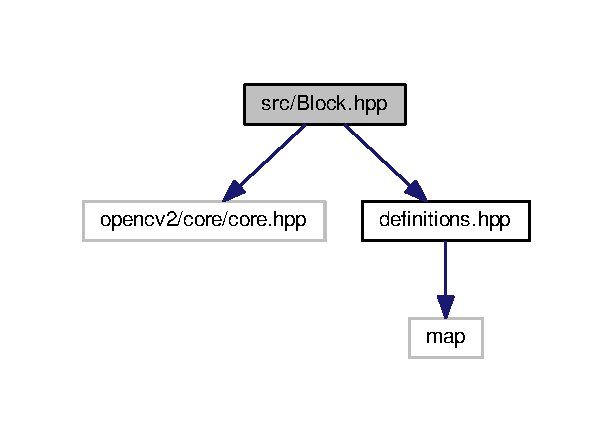
\includegraphics[width=294pt]{Block_8hpp__incl}
\end{center}
\end{figure}
This graph shows which files directly or indirectly include this file\+:
\nopagebreak
\begin{figure}[H]
\begin{center}
\leavevmode
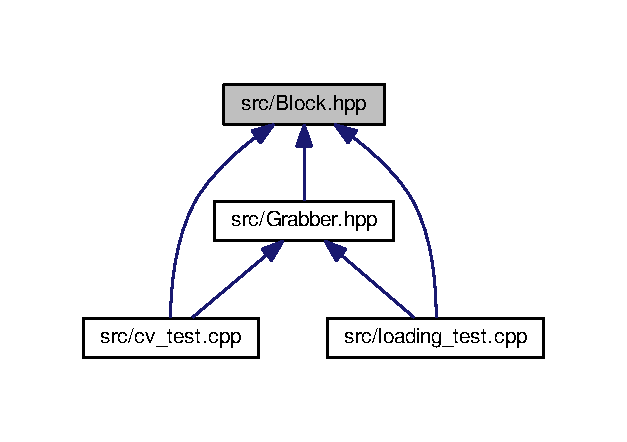
\includegraphics[width=301pt]{Block_8hpp__dep__incl}
\end{center}
\end{figure}
\subsection*{Classes}
\begin{DoxyCompactItemize}
\item 
class \hyperlink{classChipChipArray_1_1Block}{Chip\+Chip\+Array\+::\+Block}
\end{DoxyCompactItemize}
\subsection*{Namespaces}
\begin{DoxyCompactItemize}
\item 
 \hyperlink{namespaceChipChipArray}{Chip\+Chip\+Array}
\end{DoxyCompactItemize}


\subsection{Detailed Description}
Contains Block class. 

\begin{DoxyAuthor}{Author}
Samuel Andrew Wisner, \href{mailto:awisner94@gmail.com}{\tt awisner94@gmail.\+com} 
\end{DoxyAuthor}


Definition in file \hyperlink{Block_8hpp_source}{Block.\+hpp}.


\hypertarget{cv__hue_8cpp}{\section{src/cv\+\_\+hue.cpp File Reference}
\label{cv__hue_8cpp}\index{src/cv\+\_\+hue.\+cpp@{src/cv\+\_\+hue.\+cpp}}
}
{\ttfamily \#include $<$iostream$>$}\\*
{\ttfamily \#include \char`\"{}opencv2/highgui/highgui.\+hpp\char`\"{}}\\*
{\ttfamily \#include \char`\"{}opencv2/imgproc/imgproc.\+hpp\char`\"{}}\\*
{\ttfamily \#include \char`\"{}Pi\+Camera.\+hpp\char`\"{}}\\*
Include dependency graph for cv\+\_\+hue.\+cpp\+:
\nopagebreak
\begin{figure}[H]
\begin{center}
\leavevmode
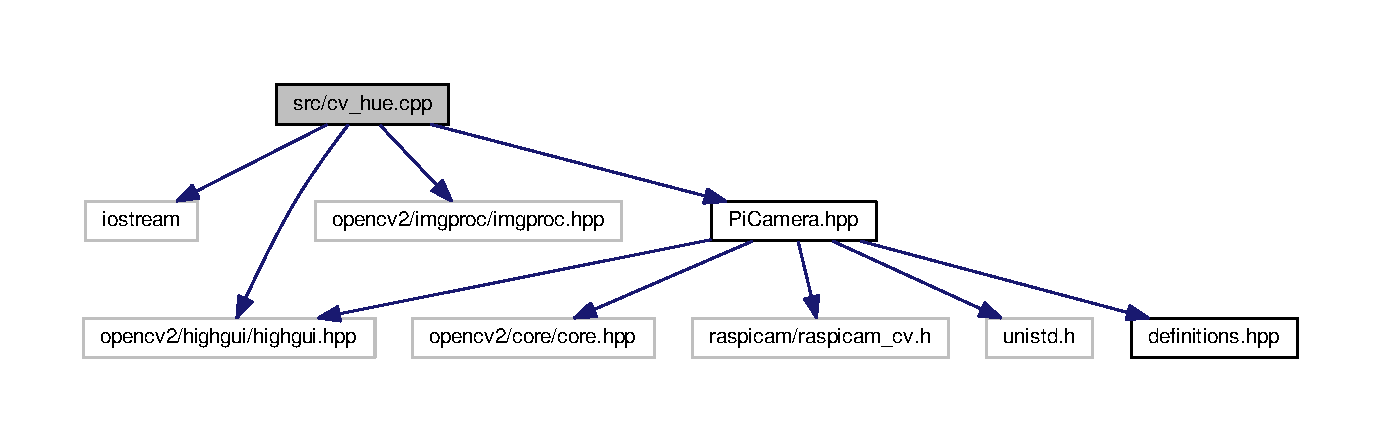
\includegraphics[width=350pt]{cv__hue_8cpp__incl}
\end{center}
\end{figure}
\subsection*{Namespaces}
\begin{DoxyCompactItemize}
\item 
 \hyperlink{namespaceChipChipArray}{Chip\+Chip\+Array}
\begin{DoxyCompactList}\small\item\em contains \hyperlink{classChipChipArray_1_1Block}{Block} class \end{DoxyCompactList}\end{DoxyCompactItemize}
\subsection*{Functions}
\begin{DoxyCompactItemize}
\item 
int \hyperlink{namespaceChipChipArray_a7fc3d1edffca11531cd09fdab7c8b88d}{Chip\+Chip\+Array\+::main} (int argc, char $\ast$$\ast$argv)
\end{DoxyCompactItemize}

\hypertarget{cv__shape_8cpp}{\section{src/cv\+\_\+shape.cpp File Reference}
\label{cv__shape_8cpp}\index{src/cv\+\_\+shape.\+cpp@{src/cv\+\_\+shape.\+cpp}}
}
{\ttfamily \#include $<$iostream$>$}\\*
{\ttfamily \#include $<$opencv2/highgui/highgui.\+hpp$>$}\\*
{\ttfamily \#include $<$opencv2/imgproc/imgproc.\+hpp$>$}\\*
{\ttfamily \#include $<$string$>$}\\*
{\ttfamily \#include \char`\"{}definitions.\+hpp\char`\"{}}\\*
{\ttfamily \#include \char`\"{}Pi\+Camera.\+hpp\char`\"{}}\\*
Include dependency graph for cv\+\_\+shape.\+cpp\+:
\nopagebreak
\begin{figure}[H]
\begin{center}
\leavevmode
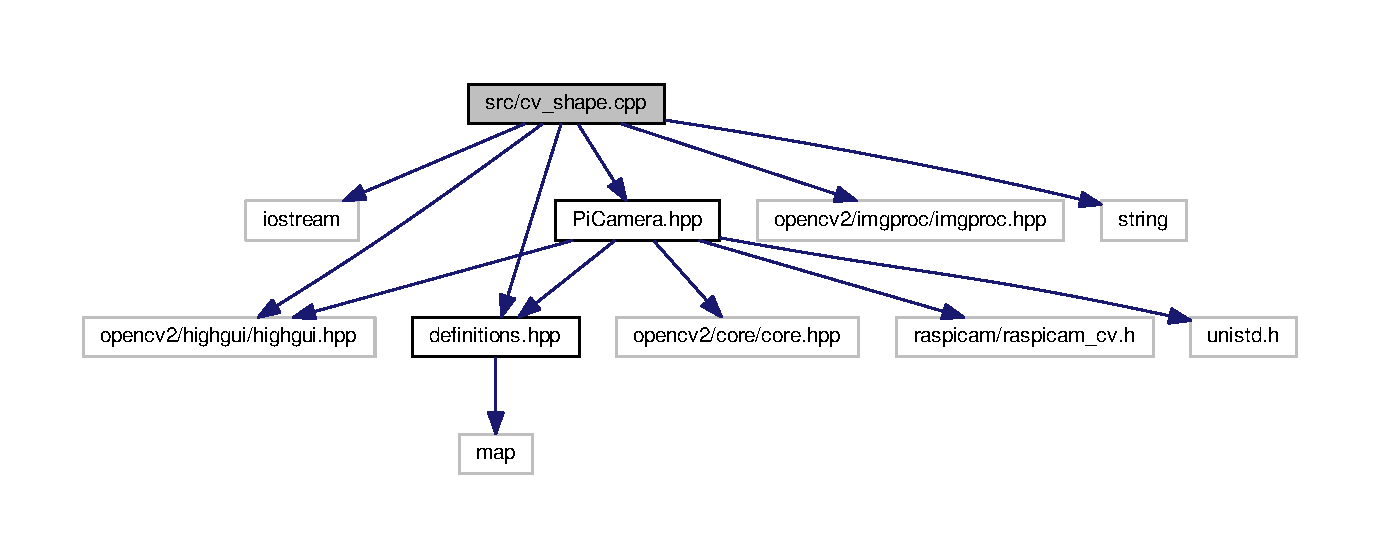
\includegraphics[width=350pt]{cv__shape_8cpp__incl}
\end{center}
\end{figure}
\subsection*{Functions}
\begin{DoxyCompactItemize}
\item 
int \hyperlink{cv__shape_8cpp_ae66f6b31b5ad750f1fe042a706a4e3d4}{main} ()
\end{DoxyCompactItemize}


\subsection{Function Documentation}
\hypertarget{cv__shape_8cpp_ae66f6b31b5ad750f1fe042a706a4e3d4}{\index{cv\+\_\+shape.\+cpp@{cv\+\_\+shape.\+cpp}!main@{main}}
\index{main@{main}!cv\+\_\+shape.\+cpp@{cv\+\_\+shape.\+cpp}}
\subsubsection[{main}]{\setlength{\rightskip}{0pt plus 5cm}int main (
\begin{DoxyParamCaption}
{}
\end{DoxyParamCaption}
)}}\label{cv__shape_8cpp_ae66f6b31b5ad750f1fe042a706a4e3d4}
This program (a single function) is a test of the computer vision algorithms for loading the blocks. It will likely be in development for some time to come. The plan currently is to develop and test all C\+V algorithms for block loading here before moving it all into class functions and testing again.

This code is based on several online articles\+:
\begin{DoxyItemize}
\item \char`\"{}\+Color Detectionn \& Object Tracking\char`\"{} by Shermal Fernando (\href{http://opencv-srf.blogspot.com/2010/09/object-detection-using-color-seperation.html}{\tt http\+://opencv-\/srf.\+blogspot.\+com/2010/09/object-\/detection-\/using-\/color-\/seperation.\+html})
\item \char`\"{}\+Shape Detection \& Tracking using Contours\char`\"{} by Shermal Fernando (\href{http://opencv-srf.blogspot.com/2011/09/object-detection-tracking-using-contours.html}{\tt http\+://opencv-\/srf.\+blogspot.\+com/2011/09/object-\/detection-\/tracking-\/using-\/contours.\+html})
\item \char`\"{}\+Creating Bounding boxes and circles for contours\char`\"{} in the Open\+C\+V 2.\+4 Tutorials (\href{http://opencv-srf.blogspot.com/2011/09/object-detection-tracking-using-contours.html}{\tt http\+://opencv-\/srf.\+blogspot.\+com/2011/09/object-\/detection-\/tracking-\/using-\/contours.\+html}) 
\end{DoxyItemize}

Definition at line 36 of file cv\+\_\+shape.\+cpp.



Here is the call graph for this function\+:
\nopagebreak
\begin{figure}[H]
\begin{center}
\leavevmode
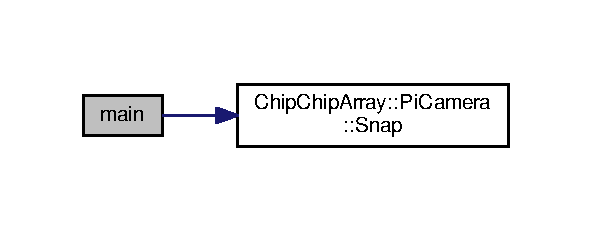
\includegraphics[width=284pt]{cv__shape_8cpp_ae66f6b31b5ad750f1fe042a706a4e3d4_cgraph}
\end{center}
\end{figure}



\hypertarget{cv__test_8cpp}{\section{src/cv\+\_\+test.cpp File Reference}
\label{cv__test_8cpp}\index{src/cv\+\_\+test.\+cpp@{src/cv\+\_\+test.\+cpp}}
}
{\ttfamily \#include $<$iostream$>$}\\*
{\ttfamily \#include \char`\"{}definitions.\+hpp\char`\"{}}\\*
{\ttfamily \#include \char`\"{}Block.\+hpp\char`\"{}}\\*
{\ttfamily \#include \char`\"{}Grabber.\+hpp\char`\"{}}\\*
Include dependency graph for cv\+\_\+test.\+cpp\+:
\nopagebreak
\begin{figure}[H]
\begin{center}
\leavevmode
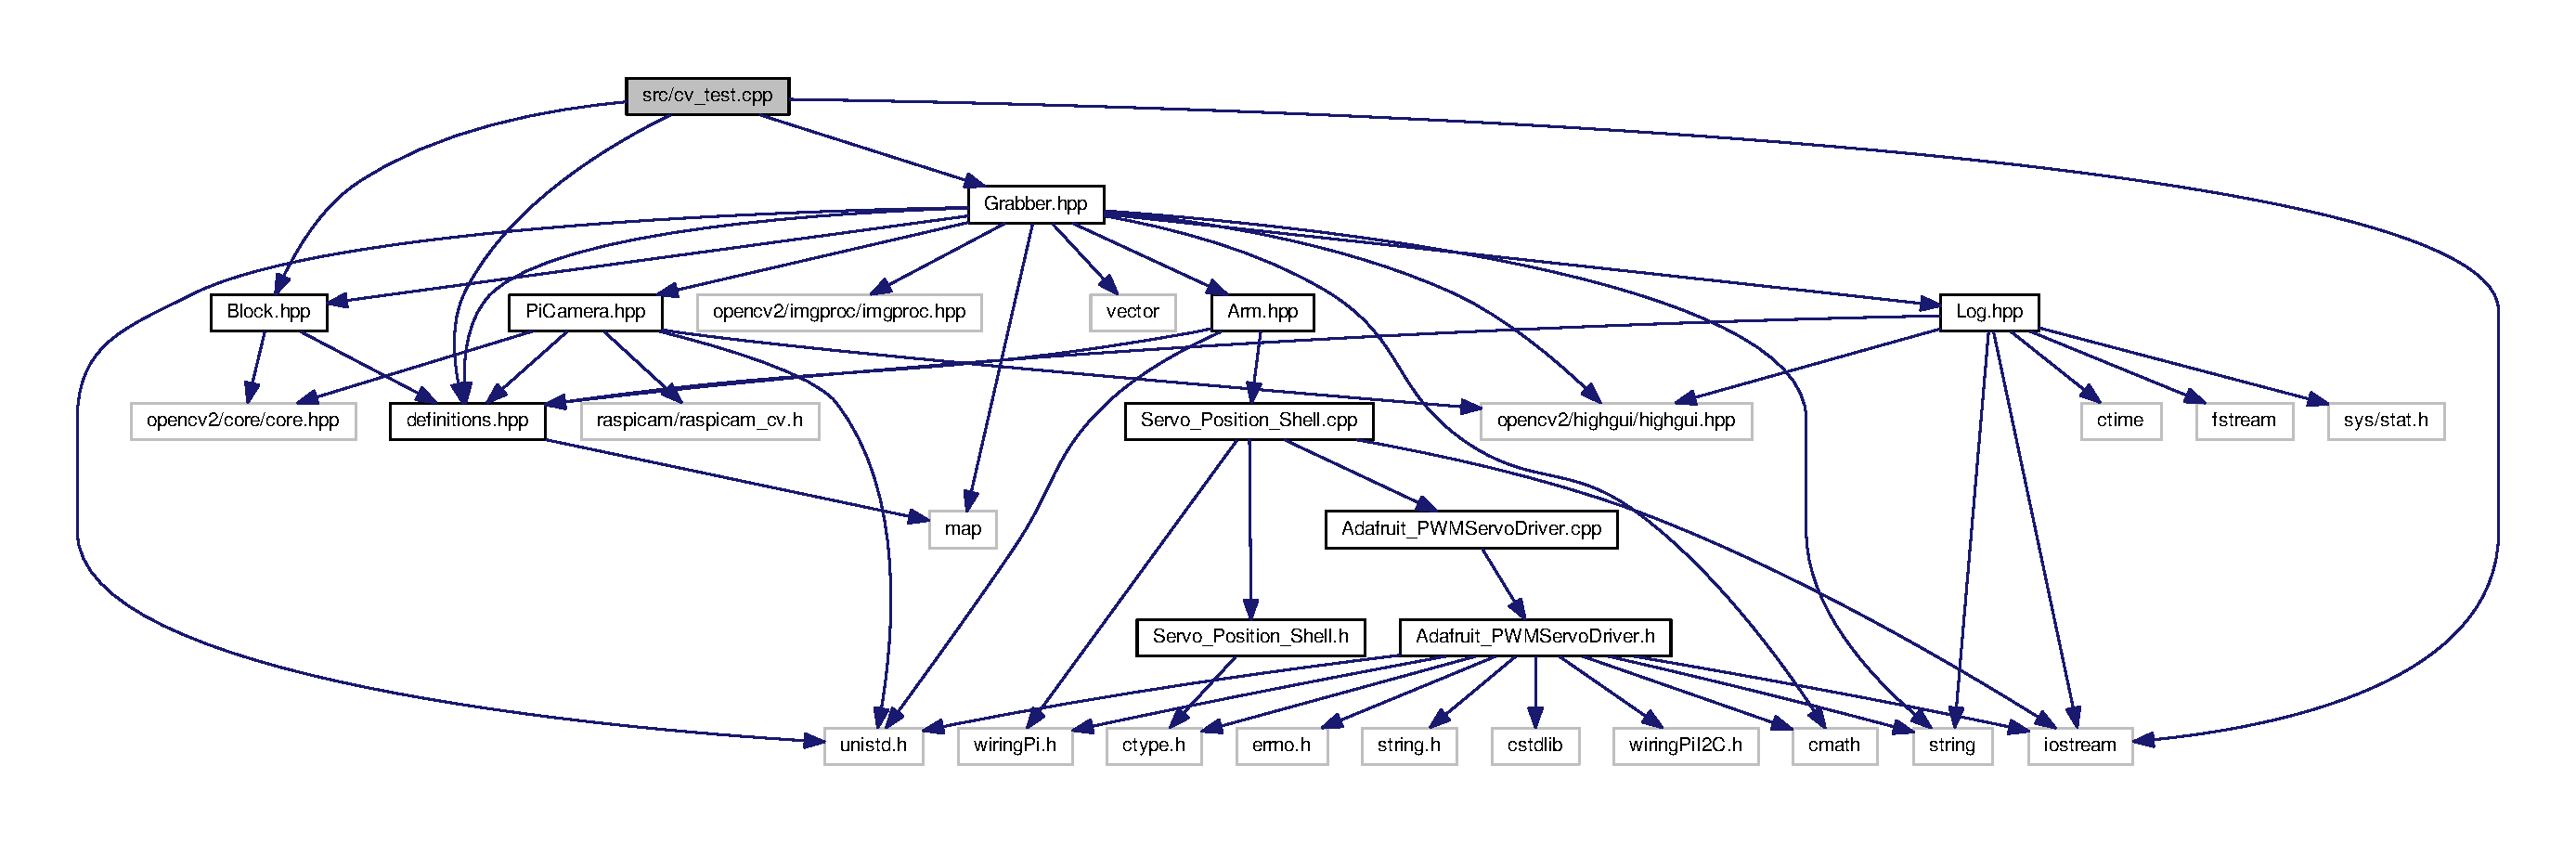
\includegraphics[width=350pt]{cv__test_8cpp__incl}
\end{center}
\end{figure}
\subsection*{Functions}
\begin{DoxyCompactItemize}
\item 
int \hyperlink{cv__test_8cpp_ae66f6b31b5ad750f1fe042a706a4e3d4}{main} ()
\end{DoxyCompactItemize}


\subsection{Function Documentation}
\hypertarget{cv__test_8cpp_ae66f6b31b5ad750f1fe042a706a4e3d4}{\index{cv\+\_\+test.\+cpp@{cv\+\_\+test.\+cpp}!main@{main}}
\index{main@{main}!cv\+\_\+test.\+cpp@{cv\+\_\+test.\+cpp}}
\subsubsection[{main}]{\setlength{\rightskip}{0pt plus 5cm}int main (
\begin{DoxyParamCaption}
{}
\end{DoxyParamCaption}
)}}\label{cv__test_8cpp_ae66f6b31b5ad750f1fe042a706a4e3d4}
This program was used solely to test the Pi\+Camera wrapper class and its compatibility with the raspicam wrapper and ultimately Open\+C\+V. 

Definition at line 18 of file cv\+\_\+test.\+cpp.



Here is the call graph for this function\+:
\nopagebreak
\begin{figure}[H]
\begin{center}
\leavevmode
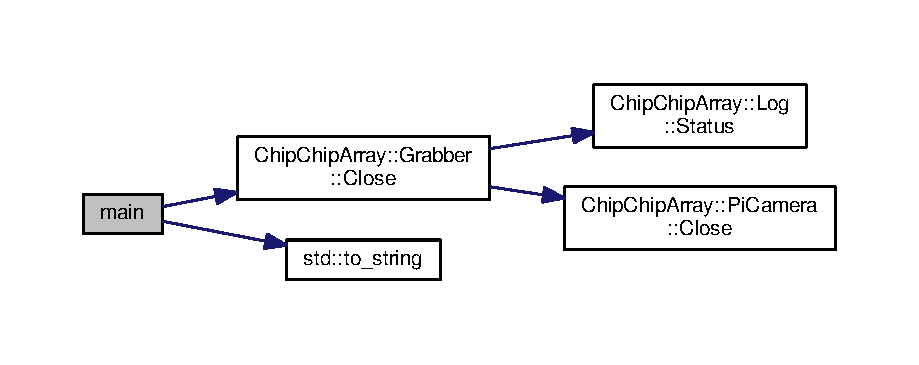
\includegraphics[width=350pt]{cv__test_8cpp_ae66f6b31b5ad750f1fe042a706a4e3d4_cgraph}
\end{center}
\end{figure}



\hypertarget{definitions_8hpp}{\section{src/definitions.hpp File Reference}
\label{definitions_8hpp}\index{src/definitions.\+hpp@{src/definitions.\+hpp}}
}
This graph shows which files directly or indirectly include this file\+:
\subsection*{Namespaces}
\begin{DoxyCompactItemize}
\item 
 \hyperlink{namespacestd}{std}
\end{DoxyCompactItemize}
\subsection*{Macros}
\begin{DoxyCompactItemize}
\item 
\#define \hyperlink{definitions_8hpp_a378181c29a641d58f55d647b5a9599f2}{E\+N\+U\+M}~signed char
\item 
\#define \hyperlink{definitions_8hpp_a8fe83ac76edc595f6b98cd4a4127aed5}{E\+R\+R\+O\+R}~-\/1
\end{DoxyCompactItemize}
\subsection*{Typedefs}
\begin{DoxyCompactItemize}
\item 
typedef unsigned char \hyperlink{definitions_8hpp_a0c8186d9b9b7880309c27230bbb5e69d}{byte}
\item 
typedef unsigned char \hyperlink{definitions_8hpp_adde6aaee8457bee49c2a92621fe22b79}{uint8}
\item 
typedef signed char \hyperlink{definitions_8hpp_a1a6408291ee3cfd0760a61ac64084154}{sint8}
\item 
typedef unsigned short \hyperlink{definitions_8hpp_a05f6b0ae8f6a6e135b0e290c25fe0e4e}{uint16}
\item 
typedef signed short \hyperlink{definitions_8hpp_a74df79fde3c518e55b29ce6360a9c76e}{sint16}
\item 
typedef unsigned int \hyperlink{definitions_8hpp_a1134b580f8da4de94ca6b1de4d37975e}{uint32}
\item 
typedef signed int \hyperlink{definitions_8hpp_a0573de65958b4fda3a0460ed417dafb8}{sint32}
\item 
typedef unsigned long long \hyperlink{definitions_8hpp_a29940ae63ec06c9998bba873e25407ad}{uint64}
\item 
typedef signed long long \hyperlink{definitions_8hpp_ad91d7e42d1c1abce1d9eeacd54cc0497}{sint64}
\item 
typedef float \hyperlink{definitions_8hpp_aacdc525d6f7bddb3ae95d5c311bd06a1}{float32}
\item 
typedef double \hyperlink{definitions_8hpp_a232fad1b0d6dcc7c16aabde98b2e2a80}{float64}
\end{DoxyCompactItemize}
\subsection*{Enumerations}
\begin{DoxyCompactItemize}
\item 
enum \hyperlink{definitions_8hpp_ac8e1b1f4bbac5914204c97f66f97d01f}{Block\+Position} \+: E\+N\+U\+M \{ \hyperlink{definitions_8hpp_ac8e1b1f4bbac5914204c97f66f97d01fa5835bab1ade0060909e31a06af2e2cde}{Block\+Position\+::\+Front}, 
\hyperlink{definitions_8hpp_ac8e1b1f4bbac5914204c97f66f97d01fa0557fa923dcee4d0f86b1409f5c2167f}{Block\+Position\+::\+Back}
 \}
\item 
enum \hyperlink{definitions_8hpp_abc05a0f46084a3477cf5d5c939ff1436}{Color} \+: E\+N\+U\+M \{ \hyperlink{definitions_8hpp_abc05a0f46084a3477cf5d5c939ff1436aee38e4d5dd68c4e440825018d549cb47}{Color\+::\+Red}, 
\hyperlink{definitions_8hpp_abc05a0f46084a3477cf5d5c939ff1436a51e6cd92b6c45f9affdc158ecca2b8b8}{Color\+::\+Yellow}, 
\hyperlink{definitions_8hpp_abc05a0f46084a3477cf5d5c939ff1436ad382816a3cbeed082c9e216e7392eed1}{Color\+::\+Green}, 
\hyperlink{definitions_8hpp_abc05a0f46084a3477cf5d5c939ff1436a9594eec95be70e7b1710f730fdda33d9}{Color\+::\+Blue}
 \}
\item 
enum \hyperlink{definitions_8hpp_aa7380b6d694cab49f07aed6a7af592d9}{Log\+Mode} \+: E\+N\+U\+M \{ \hyperlink{definitions_8hpp_aa7380b6d694cab49f07aed6a7af592d9a9dffbf69ffba8bc38bc4e01abf4b1675}{Log\+Mode\+::\+Text}, 
\hyperlink{definitions_8hpp_aa7380b6d694cab49f07aed6a7af592d9ace7898536dd0e928d1640ee2ad531cc8}{Log\+Mode\+::\+Multi}
 \}
\item 
enum \hyperlink{definitions_8hpp_ab84ebabb02540c4a7ec341a213abf1dc}{Result} \+: E\+N\+U\+M \{ \hyperlink{definitions_8hpp_ab84ebabb02540c4a7ec341a213abf1dca32075034997ab91e886dbcad47ed902d}{Result\+::\+No\+\_\+\+Blocks} = -\/1, 
\hyperlink{definitions_8hpp_ab84ebabb02540c4a7ec341a213abf1dcabdf267b7c95f2ffd040b32d8b005e9a0}{Result\+::\+No\+\_\+\+Halves} = 0, 
\hyperlink{definitions_8hpp_ab84ebabb02540c4a7ec341a213abf1dca5b00716e5e6f2e2dc1b10ffed2e0ef6d}{Result\+::\+Two\+\_\+\+Halves} = 2, 
\hyperlink{definitions_8hpp_ab84ebabb02540c4a7ec341a213abf1dca01f87e08f72dd8784d0665346a006fa3}{Result\+::\+Four\+\_\+\+Halves} = 4
 \}
\item 
enum \hyperlink{definitions_8hpp_a03325a8a9d4f105db5e37dd587128142}{Side} \+: E\+N\+U\+M \{ \hyperlink{definitions_8hpp_a03325a8a9d4f105db5e37dd587128142a945d5e233cf7d6240f6b783b36a374ff}{Side\+::\+Left}, 
\hyperlink{definitions_8hpp_a03325a8a9d4f105db5e37dd587128142a92b09c7c48c520c3c55e497875da437c}{Side\+::\+Right}
 \}
\item 
enum \hyperlink{definitions_8hpp_a9809446fd16a744b6df9808293f14153}{Size} \+: E\+N\+U\+M \{ \hyperlink{definitions_8hpp_a9809446fd16a744b6df9808293f14153a30bb747c98bccdd11b3f89e644c4d0ad}{Size\+::\+Short}, 
\hyperlink{definitions_8hpp_a9809446fd16a744b6df9808293f14153a8394f0347c184cf156ac5924dccb773b}{Size\+::\+Long}
 \}
\item 
enum \hyperlink{definitions_8hpp_adbd1e7a33d3e1751c7b2aa2562d0ecb9}{Zone} \+: E\+N\+U\+M \{ \hyperlink{definitions_8hpp_adbd1e7a33d3e1751c7b2aa2562d0ecb9a7fc56270e7a70fa81a5935b72eacbe29}{Zone\+::\+A} = 'A', 
\hyperlink{definitions_8hpp_adbd1e7a33d3e1751c7b2aa2562d0ecb9a9d5ed678fe57bcca610140957afab571}{Zone\+::\+B} = 'B', 
\hyperlink{definitions_8hpp_adbd1e7a33d3e1751c7b2aa2562d0ecb9a0d61f8370cad1d412f80b84d143e1257}{Zone\+::\+C} = 'C'
 \}
\end{DoxyCompactItemize}
\subsection*{Functions}
\begin{DoxyCompactItemize}
\item 
string \hyperlink{namespacestd_aa5ddf582a1c96ffe258c997be9a294a3}{std\+::to\+\_\+string} (\hyperlink{definitions_8hpp_ac8e1b1f4bbac5914204c97f66f97d01f}{Block\+Position} pos)
\item 
string \hyperlink{namespacestd_a6a0c3c323562edbd2f57da3d2bb74326}{std\+::to\+\_\+string} (\hyperlink{definitions_8hpp_abc05a0f46084a3477cf5d5c939ff1436}{Color} color)
\item 
string \hyperlink{namespacestd_adb24d6df94a83c325573f7710df84953}{std\+::to\+\_\+string} (\hyperlink{definitions_8hpp_aa7380b6d694cab49f07aed6a7af592d9}{Log\+Mode} mode)
\item 
string \hyperlink{namespacestd_a7fb649b1361ca7d95cc74045c0dadcdd}{std\+::to\+\_\+string} (\hyperlink{definitions_8hpp_ab84ebabb02540c4a7ec341a213abf1dc}{Result} res)
\item 
string \hyperlink{namespacestd_aae21fd95009e4cc9fa25e1ad3830980b}{std\+::to\+\_\+string} (\hyperlink{definitions_8hpp_a03325a8a9d4f105db5e37dd587128142}{Side} side)
\item 
string \hyperlink{namespacestd_a6bfcd2c3377165652c64085d7acb5c64}{std\+::to\+\_\+string} (\hyperlink{definitions_8hpp_a9809446fd16a744b6df9808293f14153}{Size} size)
\item 
string \hyperlink{namespacestd_ac50951e195256b4c2311f90189f64ba8}{std\+::to\+\_\+string} (\hyperlink{definitions_8hpp_adbd1e7a33d3e1751c7b2aa2562d0ecb9}{Zone} zone)
\end{DoxyCompactItemize}


\subsection{Macro Definition Documentation}
\hypertarget{definitions_8hpp_a378181c29a641d58f55d647b5a9599f2}{\index{definitions.\+hpp@{definitions.\+hpp}!E\+N\+U\+M@{E\+N\+U\+M}}
\index{E\+N\+U\+M@{E\+N\+U\+M}!definitions.\+hpp@{definitions.\+hpp}}
\subsubsection[{E\+N\+U\+M}]{\setlength{\rightskip}{0pt plus 5cm}\#define E\+N\+U\+M~signed char}}\label{definitions_8hpp_a378181c29a641d58f55d647b5a9599f2}


Definition at line 4 of file definitions.\+hpp.

\hypertarget{definitions_8hpp_a8fe83ac76edc595f6b98cd4a4127aed5}{\index{definitions.\+hpp@{definitions.\+hpp}!E\+R\+R\+O\+R@{E\+R\+R\+O\+R}}
\index{E\+R\+R\+O\+R@{E\+R\+R\+O\+R}!definitions.\+hpp@{definitions.\+hpp}}
\subsubsection[{E\+R\+R\+O\+R}]{\setlength{\rightskip}{0pt plus 5cm}\#define E\+R\+R\+O\+R~-\/1}}\label{definitions_8hpp_a8fe83ac76edc595f6b98cd4a4127aed5}


Definition at line 5 of file definitions.\+hpp.



\subsection{Typedef Documentation}
\hypertarget{definitions_8hpp_a0c8186d9b9b7880309c27230bbb5e69d}{\index{definitions.\+hpp@{definitions.\+hpp}!byte@{byte}}
\index{byte@{byte}!definitions.\+hpp@{definitions.\+hpp}}
\subsubsection[{byte}]{\setlength{\rightskip}{0pt plus 5cm}typedef unsigned char {\bf byte}}}\label{definitions_8hpp_a0c8186d9b9b7880309c27230bbb5e69d}


Definition at line 7 of file definitions.\+hpp.

\hypertarget{definitions_8hpp_aacdc525d6f7bddb3ae95d5c311bd06a1}{\index{definitions.\+hpp@{definitions.\+hpp}!float32@{float32}}
\index{float32@{float32}!definitions.\+hpp@{definitions.\+hpp}}
\subsubsection[{float32}]{\setlength{\rightskip}{0pt plus 5cm}typedef float {\bf float32}}}\label{definitions_8hpp_aacdc525d6f7bddb3ae95d5c311bd06a1}


Definition at line 20 of file definitions.\+hpp.

\hypertarget{definitions_8hpp_a232fad1b0d6dcc7c16aabde98b2e2a80}{\index{definitions.\+hpp@{definitions.\+hpp}!float64@{float64}}
\index{float64@{float64}!definitions.\+hpp@{definitions.\+hpp}}
\subsubsection[{float64}]{\setlength{\rightskip}{0pt plus 5cm}typedef double {\bf float64}}}\label{definitions_8hpp_a232fad1b0d6dcc7c16aabde98b2e2a80}


Definition at line 21 of file definitions.\+hpp.

\hypertarget{definitions_8hpp_a74df79fde3c518e55b29ce6360a9c76e}{\index{definitions.\+hpp@{definitions.\+hpp}!sint16@{sint16}}
\index{sint16@{sint16}!definitions.\+hpp@{definitions.\+hpp}}
\subsubsection[{sint16}]{\setlength{\rightskip}{0pt plus 5cm}typedef signed short {\bf sint16}}}\label{definitions_8hpp_a74df79fde3c518e55b29ce6360a9c76e}


Definition at line 12 of file definitions.\+hpp.

\hypertarget{definitions_8hpp_a0573de65958b4fda3a0460ed417dafb8}{\index{definitions.\+hpp@{definitions.\+hpp}!sint32@{sint32}}
\index{sint32@{sint32}!definitions.\+hpp@{definitions.\+hpp}}
\subsubsection[{sint32}]{\setlength{\rightskip}{0pt plus 5cm}typedef signed int {\bf sint32}}}\label{definitions_8hpp_a0573de65958b4fda3a0460ed417dafb8}


Definition at line 15 of file definitions.\+hpp.

\hypertarget{definitions_8hpp_ad91d7e42d1c1abce1d9eeacd54cc0497}{\index{definitions.\+hpp@{definitions.\+hpp}!sint64@{sint64}}
\index{sint64@{sint64}!definitions.\+hpp@{definitions.\+hpp}}
\subsubsection[{sint64}]{\setlength{\rightskip}{0pt plus 5cm}typedef signed long long {\bf sint64}}}\label{definitions_8hpp_ad91d7e42d1c1abce1d9eeacd54cc0497}


Definition at line 18 of file definitions.\+hpp.

\hypertarget{definitions_8hpp_a1a6408291ee3cfd0760a61ac64084154}{\index{definitions.\+hpp@{definitions.\+hpp}!sint8@{sint8}}
\index{sint8@{sint8}!definitions.\+hpp@{definitions.\+hpp}}
\subsubsection[{sint8}]{\setlength{\rightskip}{0pt plus 5cm}typedef signed char {\bf sint8}}}\label{definitions_8hpp_a1a6408291ee3cfd0760a61ac64084154}


Definition at line 9 of file definitions.\+hpp.

\hypertarget{definitions_8hpp_a05f6b0ae8f6a6e135b0e290c25fe0e4e}{\index{definitions.\+hpp@{definitions.\+hpp}!uint16@{uint16}}
\index{uint16@{uint16}!definitions.\+hpp@{definitions.\+hpp}}
\subsubsection[{uint16}]{\setlength{\rightskip}{0pt plus 5cm}typedef unsigned short {\bf uint16}}}\label{definitions_8hpp_a05f6b0ae8f6a6e135b0e290c25fe0e4e}


Definition at line 11 of file definitions.\+hpp.

\hypertarget{definitions_8hpp_a1134b580f8da4de94ca6b1de4d37975e}{\index{definitions.\+hpp@{definitions.\+hpp}!uint32@{uint32}}
\index{uint32@{uint32}!definitions.\+hpp@{definitions.\+hpp}}
\subsubsection[{uint32}]{\setlength{\rightskip}{0pt plus 5cm}typedef unsigned int {\bf uint32}}}\label{definitions_8hpp_a1134b580f8da4de94ca6b1de4d37975e}


Definition at line 14 of file definitions.\+hpp.

\hypertarget{definitions_8hpp_a29940ae63ec06c9998bba873e25407ad}{\index{definitions.\+hpp@{definitions.\+hpp}!uint64@{uint64}}
\index{uint64@{uint64}!definitions.\+hpp@{definitions.\+hpp}}
\subsubsection[{uint64}]{\setlength{\rightskip}{0pt plus 5cm}typedef unsigned long long {\bf uint64}}}\label{definitions_8hpp_a29940ae63ec06c9998bba873e25407ad}


Definition at line 17 of file definitions.\+hpp.

\hypertarget{definitions_8hpp_adde6aaee8457bee49c2a92621fe22b79}{\index{definitions.\+hpp@{definitions.\+hpp}!uint8@{uint8}}
\index{uint8@{uint8}!definitions.\+hpp@{definitions.\+hpp}}
\subsubsection[{uint8}]{\setlength{\rightskip}{0pt plus 5cm}typedef unsigned char {\bf uint8}}}\label{definitions_8hpp_adde6aaee8457bee49c2a92621fe22b79}


Definition at line 8 of file definitions.\+hpp.



\subsection{Enumeration Type Documentation}
\hypertarget{definitions_8hpp_ac8e1b1f4bbac5914204c97f66f97d01f}{\index{definitions.\+hpp@{definitions.\+hpp}!Block\+Position@{Block\+Position}}
\index{Block\+Position@{Block\+Position}!definitions.\+hpp@{definitions.\+hpp}}
\subsubsection[{Block\+Position}]{\setlength{\rightskip}{0pt plus 5cm}enum {\bf Block\+Position} \+: {\bf E\+N\+U\+M}\hspace{0.3cm}{\ttfamily [strong]}}}\label{definitions_8hpp_ac8e1b1f4bbac5914204c97f66f97d01f}
The position of the block relative to the arm. \begin{Desc}
\item[Enumerator]\par
\begin{description}
\index{Front@{Front}!definitions.\+hpp@{definitions.\+hpp}}\index{definitions.\+hpp@{definitions.\+hpp}!Front@{Front}}\item[{\em 
\hypertarget{definitions_8hpp_ac8e1b1f4bbac5914204c97f66f97d01fa5835bab1ade0060909e31a06af2e2cde}{Front}\label{definitions_8hpp_ac8e1b1f4bbac5914204c97f66f97d01fa5835bab1ade0060909e31a06af2e2cde}
}]\index{Back@{Back}!definitions.\+hpp@{definitions.\+hpp}}\index{definitions.\+hpp@{definitions.\+hpp}!Back@{Back}}\item[{\em 
\hypertarget{definitions_8hpp_ac8e1b1f4bbac5914204c97f66f97d01fa0557fa923dcee4d0f86b1409f5c2167f}{Back}\label{definitions_8hpp_ac8e1b1f4bbac5914204c97f66f97d01fa0557fa923dcee4d0f86b1409f5c2167f}
}]\end{description}
\end{Desc}


Definition at line 24 of file definitions.\+hpp.

\hypertarget{definitions_8hpp_abc05a0f46084a3477cf5d5c939ff1436}{\index{definitions.\+hpp@{definitions.\+hpp}!Color@{Color}}
\index{Color@{Color}!definitions.\+hpp@{definitions.\+hpp}}
\subsubsection[{Color}]{\setlength{\rightskip}{0pt plus 5cm}enum {\bf Color} \+: {\bf E\+N\+U\+M}\hspace{0.3cm}{\ttfamily [strong]}}}\label{definitions_8hpp_abc05a0f46084a3477cf5d5c939ff1436}
The color of a block or train car. \begin{Desc}
\item[Enumerator]\par
\begin{description}
\index{Red@{Red}!definitions.\+hpp@{definitions.\+hpp}}\index{definitions.\+hpp@{definitions.\+hpp}!Red@{Red}}\item[{\em 
\hypertarget{definitions_8hpp_abc05a0f46084a3477cf5d5c939ff1436aee38e4d5dd68c4e440825018d549cb47}{Red}\label{definitions_8hpp_abc05a0f46084a3477cf5d5c939ff1436aee38e4d5dd68c4e440825018d549cb47}
}]\index{Yellow@{Yellow}!definitions.\+hpp@{definitions.\+hpp}}\index{definitions.\+hpp@{definitions.\+hpp}!Yellow@{Yellow}}\item[{\em 
\hypertarget{definitions_8hpp_abc05a0f46084a3477cf5d5c939ff1436a51e6cd92b6c45f9affdc158ecca2b8b8}{Yellow}\label{definitions_8hpp_abc05a0f46084a3477cf5d5c939ff1436a51e6cd92b6c45f9affdc158ecca2b8b8}
}]\index{Green@{Green}!definitions.\+hpp@{definitions.\+hpp}}\index{definitions.\+hpp@{definitions.\+hpp}!Green@{Green}}\item[{\em 
\hypertarget{definitions_8hpp_abc05a0f46084a3477cf5d5c939ff1436ad382816a3cbeed082c9e216e7392eed1}{Green}\label{definitions_8hpp_abc05a0f46084a3477cf5d5c939ff1436ad382816a3cbeed082c9e216e7392eed1}
}]\index{Blue@{Blue}!definitions.\+hpp@{definitions.\+hpp}}\index{definitions.\+hpp@{definitions.\+hpp}!Blue@{Blue}}\item[{\em 
\hypertarget{definitions_8hpp_abc05a0f46084a3477cf5d5c939ff1436a9594eec95be70e7b1710f730fdda33d9}{Blue}\label{definitions_8hpp_abc05a0f46084a3477cf5d5c939ff1436a9594eec95be70e7b1710f730fdda33d9}
}]\end{description}
\end{Desc}


Definition at line 30 of file definitions.\+hpp.

\hypertarget{definitions_8hpp_aa7380b6d694cab49f07aed6a7af592d9}{\index{definitions.\+hpp@{definitions.\+hpp}!Log\+Mode@{Log\+Mode}}
\index{Log\+Mode@{Log\+Mode}!definitions.\+hpp@{definitions.\+hpp}}
\subsubsection[{Log\+Mode}]{\setlength{\rightskip}{0pt plus 5cm}enum {\bf Log\+Mode} \+: {\bf E\+N\+U\+M}\hspace{0.3cm}{\ttfamily [strong]}}}\label{definitions_8hpp_aa7380b6d694cab49f07aed6a7af592d9}
The mode in which the Log should prepare (i.\+e., text only or text and images). \begin{Desc}
\item[Enumerator]\par
\begin{description}
\index{Text@{Text}!definitions.\+hpp@{definitions.\+hpp}}\index{definitions.\+hpp@{definitions.\+hpp}!Text@{Text}}\item[{\em 
\hypertarget{definitions_8hpp_aa7380b6d694cab49f07aed6a7af592d9a9dffbf69ffba8bc38bc4e01abf4b1675}{Text}\label{definitions_8hpp_aa7380b6d694cab49f07aed6a7af592d9a9dffbf69ffba8bc38bc4e01abf4b1675}
}]\index{Multi@{Multi}!definitions.\+hpp@{definitions.\+hpp}}\index{definitions.\+hpp@{definitions.\+hpp}!Multi@{Multi}}\item[{\em 
\hypertarget{definitions_8hpp_aa7380b6d694cab49f07aed6a7af592d9ace7898536dd0e928d1640ee2ad531cc8}{Multi}\label{definitions_8hpp_aa7380b6d694cab49f07aed6a7af592d9ace7898536dd0e928d1640ee2ad531cc8}
}]\end{description}
\end{Desc}


Definition at line 41 of file definitions.\+hpp.

\hypertarget{definitions_8hpp_ab84ebabb02540c4a7ec341a213abf1dc}{\index{definitions.\+hpp@{definitions.\+hpp}!Result@{Result}}
\index{Result@{Result}!definitions.\+hpp@{definitions.\+hpp}}
\subsubsection[{Result}]{\setlength{\rightskip}{0pt plus 5cm}enum {\bf Result} \+: {\bf E\+N\+U\+M}\hspace{0.3cm}{\ttfamily [strong]}}}\label{definitions_8hpp_ab84ebabb02540c4a7ec341a213abf1dc}
The number of half blocks picked up in a stack. The integer value of the \begin{Desc}
\item[Enumerator]\par
\begin{description}
\index{No\+\_\+\+Blocks@{No\+\_\+\+Blocks}!definitions.\+hpp@{definitions.\+hpp}}\index{definitions.\+hpp@{definitions.\+hpp}!No\+\_\+\+Blocks@{No\+\_\+\+Blocks}}\item[{\em 
\hypertarget{definitions_8hpp_ab84ebabb02540c4a7ec341a213abf1dca32075034997ab91e886dbcad47ed902d}{No\+\_\+\+Blocks}\label{definitions_8hpp_ab84ebabb02540c4a7ec341a213abf1dca32075034997ab91e886dbcad47ed902d}
}]\index{No\+\_\+\+Halves@{No\+\_\+\+Halves}!definitions.\+hpp@{definitions.\+hpp}}\index{definitions.\+hpp@{definitions.\+hpp}!No\+\_\+\+Halves@{No\+\_\+\+Halves}}\item[{\em 
\hypertarget{definitions_8hpp_ab84ebabb02540c4a7ec341a213abf1dcabdf267b7c95f2ffd040b32d8b005e9a0}{No\+\_\+\+Halves}\label{definitions_8hpp_ab84ebabb02540c4a7ec341a213abf1dcabdf267b7c95f2ffd040b32d8b005e9a0}
}]\index{Two\+\_\+\+Halves@{Two\+\_\+\+Halves}!definitions.\+hpp@{definitions.\+hpp}}\index{definitions.\+hpp@{definitions.\+hpp}!Two\+\_\+\+Halves@{Two\+\_\+\+Halves}}\item[{\em 
\hypertarget{definitions_8hpp_ab84ebabb02540c4a7ec341a213abf1dca5b00716e5e6f2e2dc1b10ffed2e0ef6d}{Two\+\_\+\+Halves}\label{definitions_8hpp_ab84ebabb02540c4a7ec341a213abf1dca5b00716e5e6f2e2dc1b10ffed2e0ef6d}
}]\index{Four\+\_\+\+Halves@{Four\+\_\+\+Halves}!definitions.\+hpp@{definitions.\+hpp}}\index{definitions.\+hpp@{definitions.\+hpp}!Four\+\_\+\+Halves@{Four\+\_\+\+Halves}}\item[{\em 
\hypertarget{definitions_8hpp_ab84ebabb02540c4a7ec341a213abf1dca01f87e08f72dd8784d0665346a006fa3}{Four\+\_\+\+Halves}\label{definitions_8hpp_ab84ebabb02540c4a7ec341a213abf1dca01f87e08f72dd8784d0665346a006fa3}
}]\end{description}
\end{Desc}


Definition at line 50 of file definitions.\+hpp.

\hypertarget{definitions_8hpp_a03325a8a9d4f105db5e37dd587128142}{\index{definitions.\+hpp@{definitions.\+hpp}!Side@{Side}}
\index{Side@{Side}!definitions.\+hpp@{definitions.\+hpp}}
\subsubsection[{Side}]{\setlength{\rightskip}{0pt plus 5cm}enum {\bf Side} \+: {\bf E\+N\+U\+M}\hspace{0.3cm}{\ttfamily [strong]}}}\label{definitions_8hpp_a03325a8a9d4f105db5e37dd587128142}
Represents which block to pick up when multiple blocks are visible. \begin{Desc}
\item[Enumerator]\par
\begin{description}
\index{Left@{Left}!definitions.\+hpp@{definitions.\+hpp}}\index{definitions.\+hpp@{definitions.\+hpp}!Left@{Left}}\item[{\em 
\hypertarget{definitions_8hpp_a03325a8a9d4f105db5e37dd587128142a945d5e233cf7d6240f6b783b36a374ff}{Left}\label{definitions_8hpp_a03325a8a9d4f105db5e37dd587128142a945d5e233cf7d6240f6b783b36a374ff}
}]\index{Right@{Right}!definitions.\+hpp@{definitions.\+hpp}}\index{definitions.\+hpp@{definitions.\+hpp}!Right@{Right}}\item[{\em 
\hypertarget{definitions_8hpp_a03325a8a9d4f105db5e37dd587128142a92b09c7c48c520c3c55e497875da437c}{Right}\label{definitions_8hpp_a03325a8a9d4f105db5e37dd587128142a92b09c7c48c520c3c55e497875da437c}
}]\end{description}
\end{Desc}


Definition at line 58 of file definitions.\+hpp.

\hypertarget{definitions_8hpp_a9809446fd16a744b6df9808293f14153}{\index{definitions.\+hpp@{definitions.\+hpp}!Size@{Size}}
\index{Size@{Size}!definitions.\+hpp@{definitions.\+hpp}}
\subsubsection[{Size}]{\setlength{\rightskip}{0pt plus 5cm}enum {\bf Size} \+: {\bf E\+N\+U\+M}\hspace{0.3cm}{\ttfamily [strong]}}}\label{definitions_8hpp_a9809446fd16a744b6df9808293f14153}
The block size, either 2.\+5\char`\"{} or 5\char`\"{}. \begin{Desc}
\item[Enumerator]\par
\begin{description}
\index{Short@{Short}!definitions.\+hpp@{definitions.\+hpp}}\index{definitions.\+hpp@{definitions.\+hpp}!Short@{Short}}\item[{\em 
\hypertarget{definitions_8hpp_a9809446fd16a744b6df9808293f14153a30bb747c98bccdd11b3f89e644c4d0ad}{Short}\label{definitions_8hpp_a9809446fd16a744b6df9808293f14153a30bb747c98bccdd11b3f89e644c4d0ad}
}]\index{Long@{Long}!definitions.\+hpp@{definitions.\+hpp}}\index{definitions.\+hpp@{definitions.\+hpp}!Long@{Long}}\item[{\em 
\hypertarget{definitions_8hpp_a9809446fd16a744b6df9808293f14153a8394f0347c184cf156ac5924dccb773b}{Long}\label{definitions_8hpp_a9809446fd16a744b6df9808293f14153a8394f0347c184cf156ac5924dccb773b}
}]\end{description}
\end{Desc}


Definition at line 64 of file definitions.\+hpp.

\hypertarget{definitions_8hpp_adbd1e7a33d3e1751c7b2aa2562d0ecb9}{\index{definitions.\+hpp@{definitions.\+hpp}!Zone@{Zone}}
\index{Zone@{Zone}!definitions.\+hpp@{definitions.\+hpp}}
\subsubsection[{Zone}]{\setlength{\rightskip}{0pt plus 5cm}enum {\bf Zone} \+: {\bf E\+N\+U\+M}\hspace{0.3cm}{\ttfamily [strong]}}}\label{definitions_8hpp_adbd1e7a33d3e1751c7b2aa2562d0ecb9}
Zone A, B, or C \begin{Desc}
\item[Enumerator]\par
\begin{description}
\index{A@{A}!definitions.\+hpp@{definitions.\+hpp}}\index{definitions.\+hpp@{definitions.\+hpp}!A@{A}}\item[{\em 
\hypertarget{definitions_8hpp_adbd1e7a33d3e1751c7b2aa2562d0ecb9a7fc56270e7a70fa81a5935b72eacbe29}{A}\label{definitions_8hpp_adbd1e7a33d3e1751c7b2aa2562d0ecb9a7fc56270e7a70fa81a5935b72eacbe29}
}]\index{B@{B}!definitions.\+hpp@{definitions.\+hpp}}\index{definitions.\+hpp@{definitions.\+hpp}!B@{B}}\item[{\em 
\hypertarget{definitions_8hpp_adbd1e7a33d3e1751c7b2aa2562d0ecb9a9d5ed678fe57bcca610140957afab571}{B}\label{definitions_8hpp_adbd1e7a33d3e1751c7b2aa2562d0ecb9a9d5ed678fe57bcca610140957afab571}
}]\index{C@{C}!definitions.\+hpp@{definitions.\+hpp}}\index{definitions.\+hpp@{definitions.\+hpp}!C@{C}}\item[{\em 
\hypertarget{definitions_8hpp_adbd1e7a33d3e1751c7b2aa2562d0ecb9a0d61f8370cad1d412f80b84d143e1257}{C}\label{definitions_8hpp_adbd1e7a33d3e1751c7b2aa2562d0ecb9a0d61f8370cad1d412f80b84d143e1257}
}]\end{description}
\end{Desc}


Definition at line 70 of file definitions.\+hpp.


\hypertarget{Grabber_8hpp}{\section{src/\+Grabber.hpp File Reference}
\label{Grabber_8hpp}\index{src/\+Grabber.\+hpp@{src/\+Grabber.\+hpp}}
}
{\ttfamily \#include $<$cmath$>$}\\*
{\ttfamily \#include $<$map$>$}\\*
{\ttfamily \#include $<$opencv2/highgui/highgui.\+hpp$>$}\\*
{\ttfamily \#include $<$opencv2/imgproc/imgproc.\+hpp$>$}\\*
{\ttfamily \#include $<$string$>$}\\*
{\ttfamily \#include $<$unistd.\+h$>$}\\*
{\ttfamily \#include $<$vector$>$}\\*
{\ttfamily \#include \char`\"{}Arm.\+hpp\char`\"{}}\\*
{\ttfamily \#include \char`\"{}definitions.\+hpp\char`\"{}}\\*
{\ttfamily \#include \char`\"{}Block.\+hpp\char`\"{}}\\*
{\ttfamily \#include \char`\"{}Log.\+hpp\char`\"{}}\\*
{\ttfamily \#include \char`\"{}Pi\+Camera.\+hpp\char`\"{}}\\*
Include dependency graph for Grabber.\+hpp\+:
\nopagebreak
\begin{figure}[H]
\begin{center}
\leavevmode
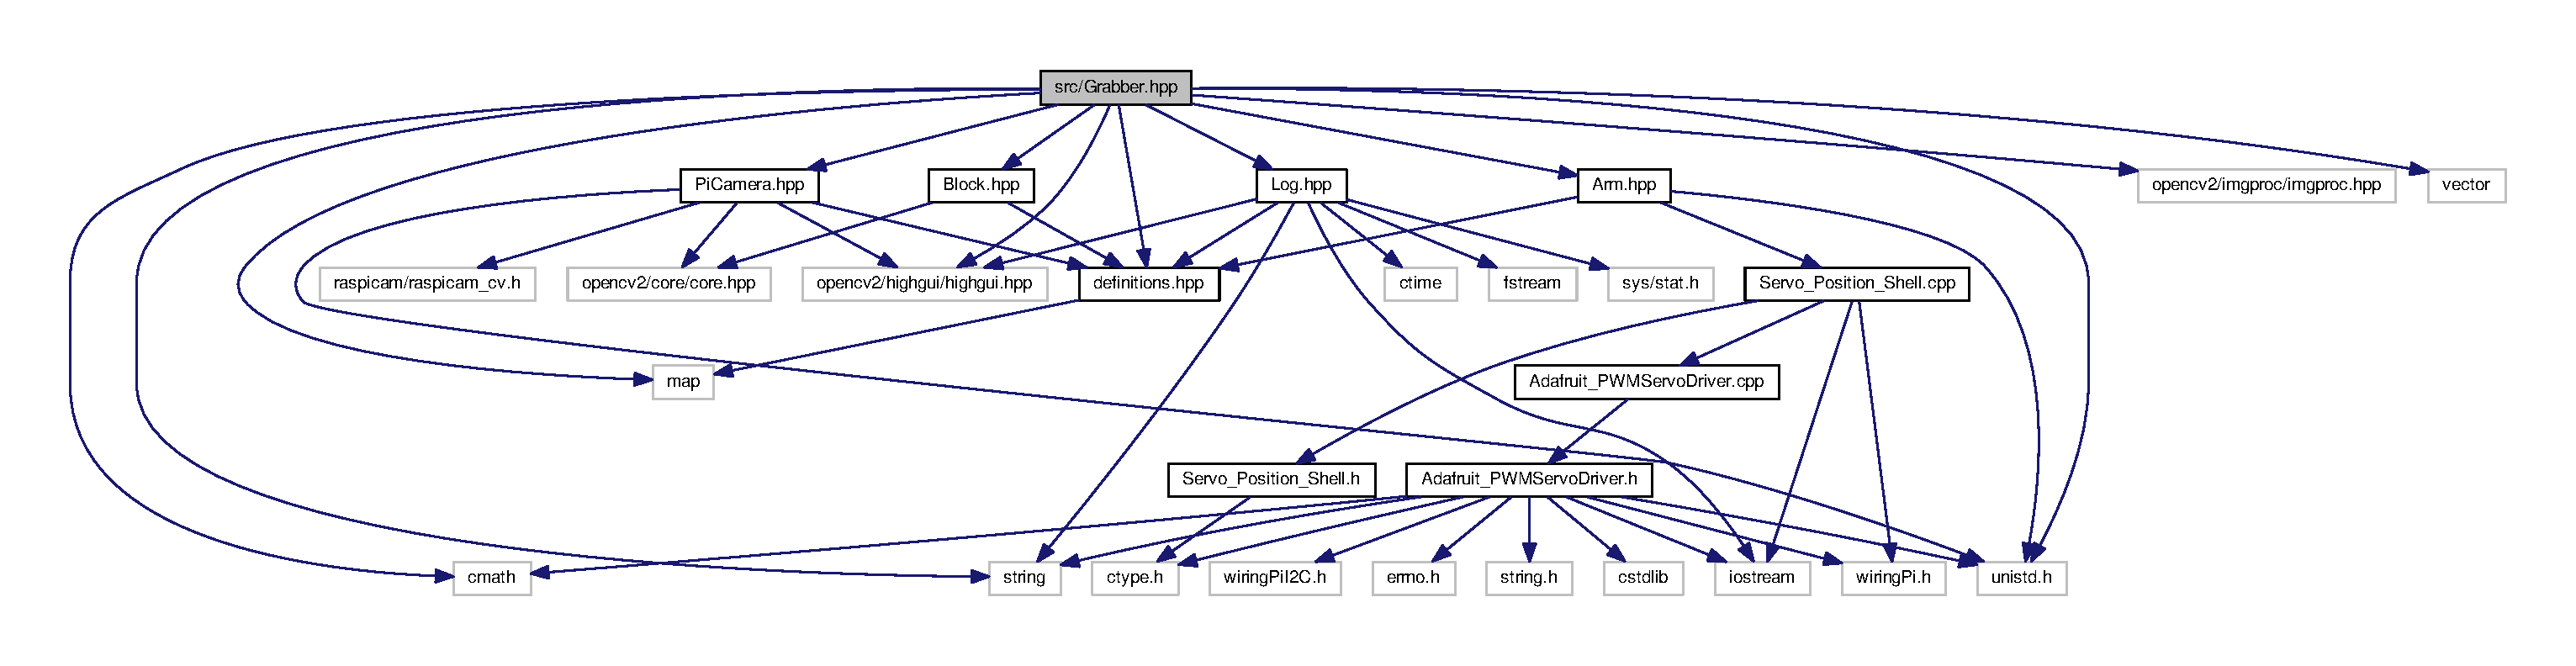
\includegraphics[width=350pt]{Grabber_8hpp__incl}
\end{center}
\end{figure}
This graph shows which files directly or indirectly include this file\+:
\nopagebreak
\begin{figure}[H]
\begin{center}
\leavevmode
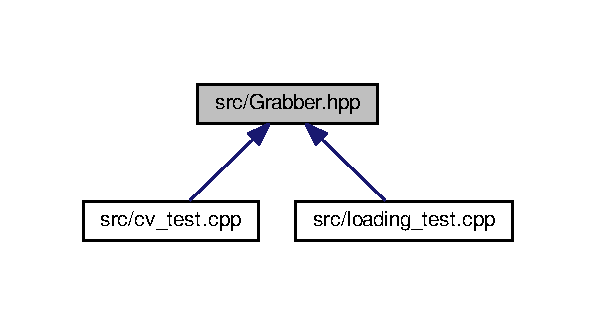
\includegraphics[width=286pt]{Grabber_8hpp__dep__incl}
\end{center}
\end{figure}
\subsection*{Classes}
\begin{DoxyCompactItemize}
\item 
class \hyperlink{classChipChipArray_1_1Grabber}{Chip\+Chip\+Array\+::\+Grabber}
\end{DoxyCompactItemize}
\subsection*{Namespaces}
\begin{DoxyCompactItemize}
\item 
 \hyperlink{namespaceChipChipArray}{Chip\+Chip\+Array}
\begin{DoxyCompactList}\small\item\em contains \hyperlink{classChipChipArray_1_1Block}{Block} class \end{DoxyCompactList}\end{DoxyCompactItemize}

\hypertarget{Log_8hpp}{\section{src/\+Log.hpp File Reference}
\label{Log_8hpp}\index{src/\+Log.\+hpp@{src/\+Log.\+hpp}}
}


Contains Log class.  


{\ttfamily \#include $<$ctime$>$}\\*
{\ttfamily \#include $<$fstream$>$}\\*
{\ttfamily \#include $<$iostream$>$}\\*
{\ttfamily \#include $<$opencv2/highgui/highgui.\+hpp$>$}\\*
{\ttfamily \#include $<$string$>$}\\*
{\ttfamily \#include $<$sys/stat.\+h$>$}\\*
{\ttfamily \#include \char`\"{}definitions.\+hpp\char`\"{}}\\*
Include dependency graph for Log.\+hpp\+:
\nopagebreak
\begin{figure}[H]
\begin{center}
\leavevmode
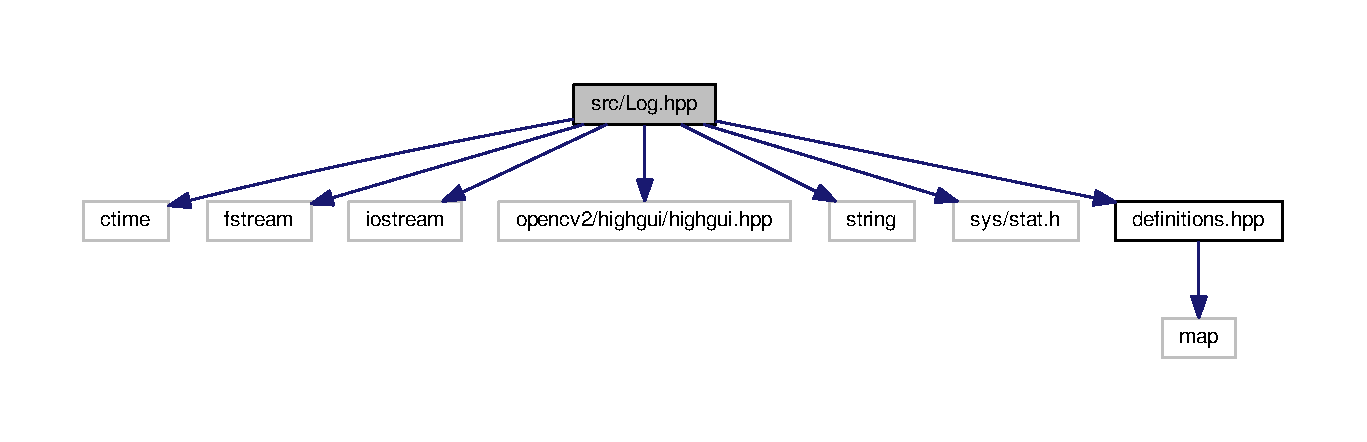
\includegraphics[width=350pt]{Log_8hpp__incl}
\end{center}
\end{figure}
This graph shows which files directly or indirectly include this file\+:
\nopagebreak
\begin{figure}[H]
\begin{center}
\leavevmode
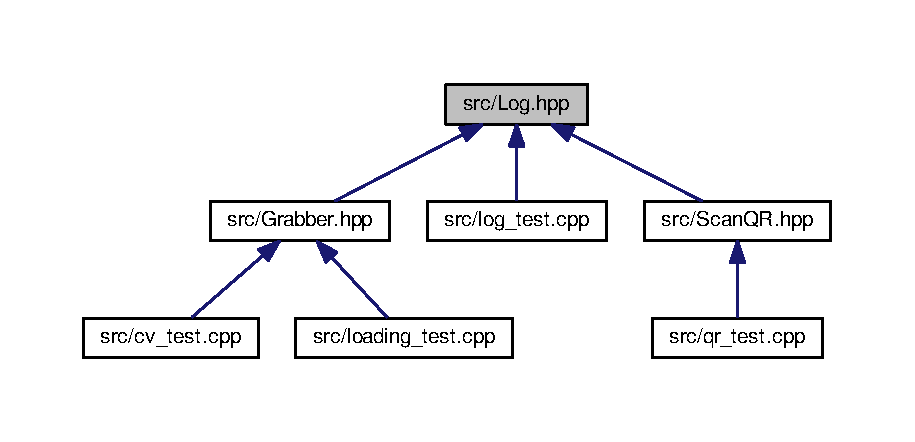
\includegraphics[width=350pt]{Log_8hpp__dep__incl}
\end{center}
\end{figure}
\subsection*{Classes}
\begin{DoxyCompactItemize}
\item 
class \hyperlink{classChipChipArray_1_1Log}{Chip\+Chip\+Array\+::\+Log}
\end{DoxyCompactItemize}
\subsection*{Namespaces}
\begin{DoxyCompactItemize}
\item 
 \hyperlink{namespaceChipChipArray}{Chip\+Chip\+Array}
\end{DoxyCompactItemize}


\subsection{Detailed Description}
Contains Log class. 

\begin{DoxyAuthor}{Author}
Samuel Andrew Wisner, \href{mailto:awisner94@gmail.com}{\tt awisner94@gmail.\+com} 
\end{DoxyAuthor}


Definition in file \hyperlink{Log_8hpp_source}{Log.\+hpp}.


\hypertarget{log__test_8cpp}{\section{src/log\+\_\+test.cpp File Reference}
\label{log__test_8cpp}\index{src/log\+\_\+test.\+cpp@{src/log\+\_\+test.\+cpp}}
}
{\ttfamily \#include $<$iostream$>$}\\*
{\ttfamily \#include $<$sstream$>$}\\*
{\ttfamily \#include $<$string$>$}\\*
{\ttfamily \#include \char`\"{}definitions.\+hpp\char`\"{}}\\*
{\ttfamily \#include \char`\"{}Log.\+hpp\char`\"{}}\\*
Include dependency graph for log\+\_\+test.\+cpp\+:
\subsection*{Functions}
\begin{DoxyCompactItemize}
\item 
int \hyperlink{log__test_8cpp_ae66f6b31b5ad750f1fe042a706a4e3d4}{main} ()
\end{DoxyCompactItemize}


\subsection{Function Documentation}
\hypertarget{log__test_8cpp_ae66f6b31b5ad750f1fe042a706a4e3d4}{\index{log\+\_\+test.\+cpp@{log\+\_\+test.\+cpp}!main@{main}}
\index{main@{main}!log\+\_\+test.\+cpp@{log\+\_\+test.\+cpp}}
\subsubsection[{main}]{\setlength{\rightskip}{0pt plus 5cm}int main (
\begin{DoxyParamCaption}
{}
\end{DoxyParamCaption}
)}}\label{log__test_8cpp_ae66f6b31b5ad750f1fe042a706a4e3d4}
This program partially tests the Log class. 

Definition at line 12 of file log\+\_\+test.\+cpp.



Here is the call graph for this function\+:



\hypertarget{main_8cpp}{\section{src/main.cpp File Reference}
\label{main_8cpp}\index{src/main.\+cpp@{src/main.\+cpp}}
}
{\ttfamily \#include $<$cstdlib$>$}\\*
{\ttfamily \#include $<$unistd.\+h$>$}\\*
{\ttfamily \#include \char`\"{}Servo\+\_\+\+Position\+\_\+\+Shell.\+h\char`\"{}}\\*
{\ttfamily \#include \char`\"{}Adafruit\+\_\+\+P\+W\+M\+Servo\+Driver.\+h\char`\"{}}\\*
{\ttfamily \#include $<$iostream$>$}\\*
{\ttfamily \#include $<$map$>$}\\*
{\ttfamily \#include \char`\"{}Navigation\+Control.\+h\char`\"{}}\\*
Include dependency graph for main.\+cpp\+:
\nopagebreak
\begin{figure}[H]
\begin{center}
\leavevmode
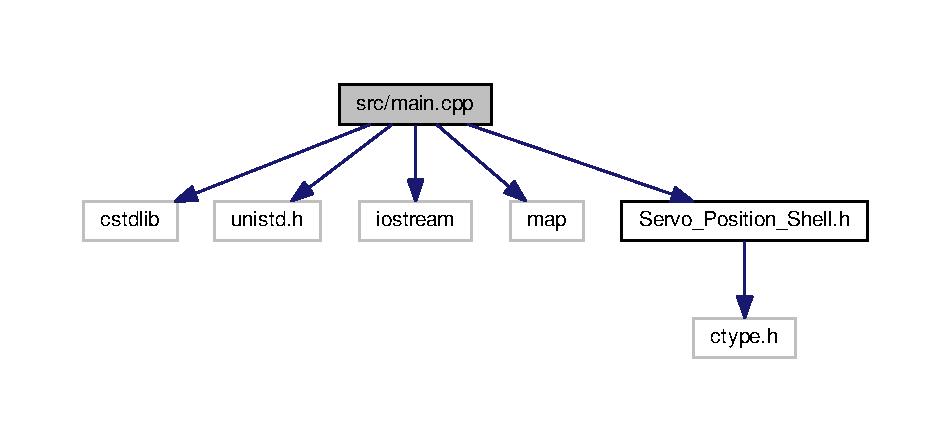
\includegraphics[width=350pt]{main_8cpp__incl}
\end{center}
\end{figure}
\subsection*{Macros}
\begin{DoxyCompactItemize}
\item 
\#define \hyperlink{main_8cpp_a33be95e76777822717adaa706897dba9}{A\+R\+M\+T\+E\+S\+T}
\end{DoxyCompactItemize}
\subsection*{Functions}
\begin{DoxyCompactItemize}
\item 
int \hyperlink{main_8cpp_ae66f6b31b5ad750f1fe042a706a4e3d4}{main} ()
\end{DoxyCompactItemize}


\subsection{Macro Definition Documentation}
\hypertarget{main_8cpp_a33be95e76777822717adaa706897dba9}{\index{main.\+cpp@{main.\+cpp}!A\+R\+M\+T\+E\+S\+T@{A\+R\+M\+T\+E\+S\+T}}
\index{A\+R\+M\+T\+E\+S\+T@{A\+R\+M\+T\+E\+S\+T}!main.\+cpp@{main.\+cpp}}
\subsubsection[{A\+R\+M\+T\+E\+S\+T}]{\setlength{\rightskip}{0pt plus 5cm}\#define A\+R\+M\+T\+E\+S\+T}}\label{main_8cpp_a33be95e76777822717adaa706897dba9}


Definition at line 16 of file main.\+cpp.



\subsection{Function Documentation}
\hypertarget{main_8cpp_ae66f6b31b5ad750f1fe042a706a4e3d4}{\index{main.\+cpp@{main.\+cpp}!main@{main}}
\index{main@{main}!main.\+cpp@{main.\+cpp}}
\subsubsection[{main}]{\setlength{\rightskip}{0pt plus 5cm}int main (
\begin{DoxyParamCaption}
{}
\end{DoxyParamCaption}
)}}\label{main_8cpp_ae66f6b31b5ad750f1fe042a706a4e3d4}


Definition at line 23 of file main.\+cpp.



Here is the call graph for this function\+:
\nopagebreak
\begin{figure}[H]
\begin{center}
\leavevmode
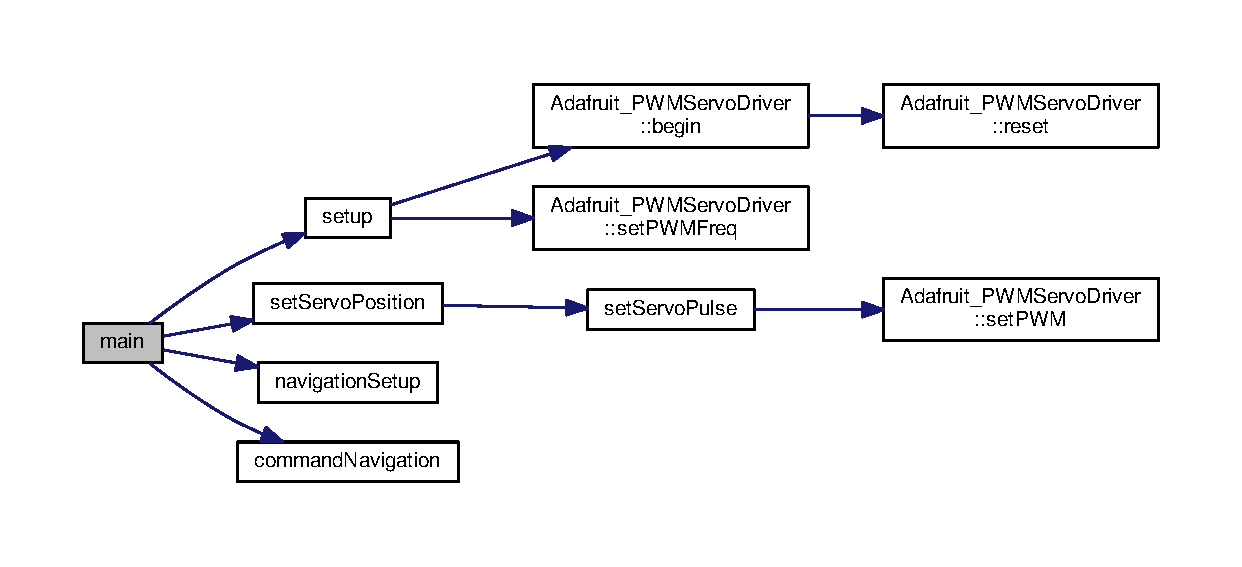
\includegraphics[width=350pt]{main_8cpp_ae66f6b31b5ad750f1fe042a706a4e3d4_cgraph}
\end{center}
\end{figure}



\hypertarget{net__qr__test_8cpp}{\section{src/net\+\_\+qr\+\_\+test.cpp File Reference}
\label{net__qr__test_8cpp}\index{src/net\+\_\+qr\+\_\+test.\+cpp@{src/net\+\_\+qr\+\_\+test.\+cpp}}
}
{\ttfamily \#include $<$opencv2/highgui/highgui.\+hpp$>$}\\*
{\ttfamily \#include $<$opencv2/imgproc/imgproc.\+hpp$>$}\\*
{\ttfamily \#include $<$zbar.\+h$>$}\\*
{\ttfamily \#include $<$iostream$>$}\\*
{\ttfamily \#include \char`\"{}Pi\+Camera.\+hpp\char`\"{}}\\*
Include dependency graph for net\+\_\+qr\+\_\+test.\+cpp\+:
\nopagebreak
\begin{figure}[H]
\begin{center}
\leavevmode
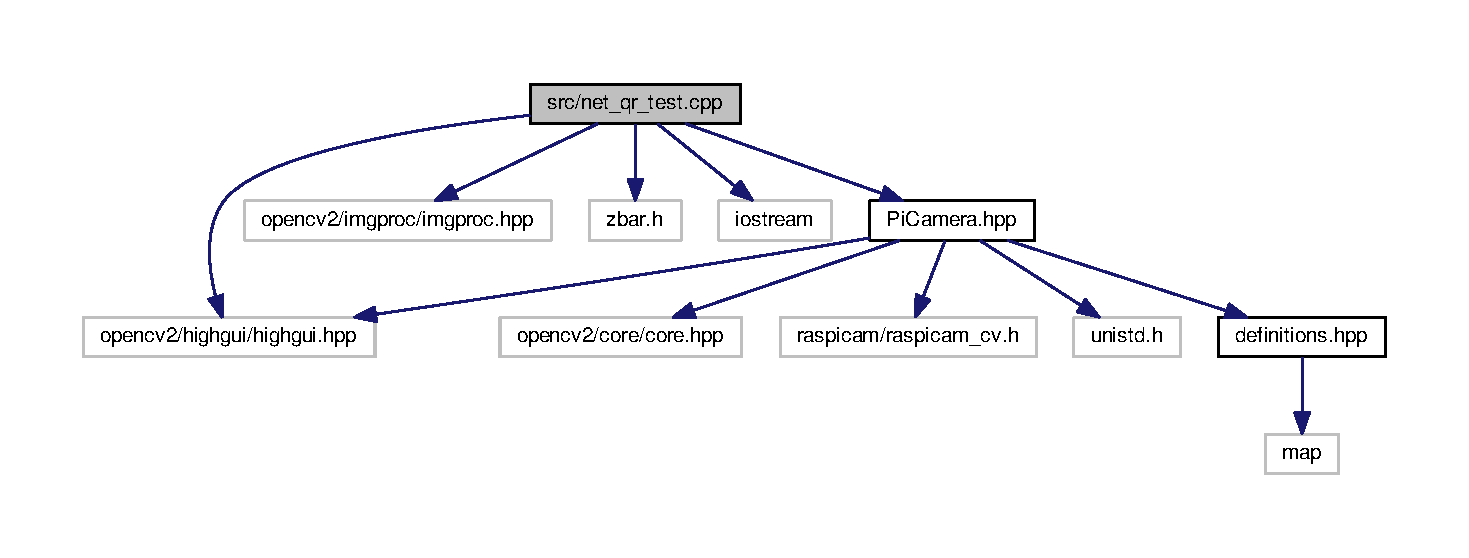
\includegraphics[width=350pt]{net__qr__test_8cpp__incl}
\end{center}
\end{figure}
\subsection*{Functions}
\begin{DoxyCompactItemize}
\item 
int \hyperlink{net__qr__test_8cpp_a0ddf1224851353fc92bfbff6f499fa97}{main} (int argc, char $\ast$argv\mbox{[}$\,$\mbox{]})
\end{DoxyCompactItemize}


\subsection{Function Documentation}
\hypertarget{net__qr__test_8cpp_a0ddf1224851353fc92bfbff6f499fa97}{\index{net\+\_\+qr\+\_\+test.\+cpp@{net\+\_\+qr\+\_\+test.\+cpp}!main@{main}}
\index{main@{main}!net\+\_\+qr\+\_\+test.\+cpp@{net\+\_\+qr\+\_\+test.\+cpp}}
\subsubsection[{main}]{\setlength{\rightskip}{0pt plus 5cm}int main (
\begin{DoxyParamCaption}
\item[{int}]{argc, }
\item[{char $\ast$}]{argv\mbox{[}$\,$\mbox{]}}
\end{DoxyParamCaption}
)}}\label{net__qr__test_8cpp_a0ddf1224851353fc92bfbff6f499fa97}
This is a (modified) test program written by Michael Young (\href{https://github.com/ayoungprogrammer/WebcamCodeScanner}{\tt https\+://github.\+com/ayoungprogrammer/\+Webcam\+Code\+Scanner}). It was modified to work with the Raspicam. 

Definition at line 24 of file net\+\_\+qr\+\_\+test.\+cpp.



Here is the call graph for this function\+:
\nopagebreak
\begin{figure}[H]
\begin{center}
\leavevmode
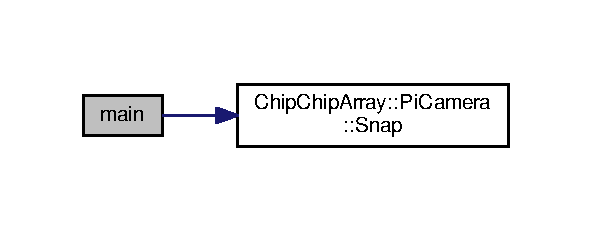
\includegraphics[width=284pt]{net__qr__test_8cpp_a0ddf1224851353fc92bfbff6f499fa97_cgraph}
\end{center}
\end{figure}



\hypertarget{old__cv__test_8cpp}{\section{src/old\+\_\+cv\+\_\+test.cpp File Reference}
\label{old__cv__test_8cpp}\index{src/old\+\_\+cv\+\_\+test.\+cpp@{src/old\+\_\+cv\+\_\+test.\+cpp}}
}
{\ttfamily \#include $<$core/core.\+hpp$>$}\\*
{\ttfamily \#include $<$highgui/highgui.\+hpp$>$}\\*
{\ttfamily \#include $<$iostream$>$}\\*
{\ttfamily \#include \char`\"{}raspicam\+\_\+cv.\+h\char`\"{}}\\*
Include dependency graph for old\+\_\+cv\+\_\+test.\+cpp\+:
\nopagebreak
\begin{figure}[H]
\begin{center}
\leavevmode
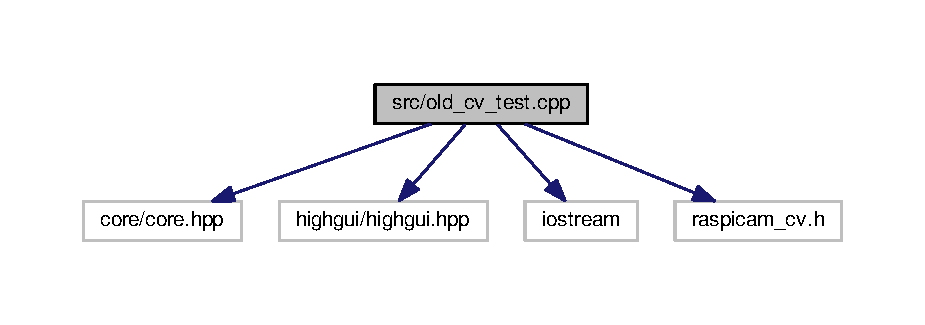
\includegraphics[width=350pt]{old__cv__test_8cpp__incl}
\end{center}
\end{figure}
\subsection*{Functions}
\begin{DoxyCompactItemize}
\item 
int \hyperlink{old__cv__test_8cpp_ae66f6b31b5ad750f1fe042a706a4e3d4}{main} ()
\begin{DoxyCompactList}\small\item\em contains old test program for the Raspi\+Cam\+\_\+\+Cv class \end{DoxyCompactList}\end{DoxyCompactItemize}


\subsection{Function Documentation}
\hypertarget{old__cv__test_8cpp_ae66f6b31b5ad750f1fe042a706a4e3d4}{\index{old\+\_\+cv\+\_\+test.\+cpp@{old\+\_\+cv\+\_\+test.\+cpp}!main@{main}}
\index{main@{main}!old\+\_\+cv\+\_\+test.\+cpp@{old\+\_\+cv\+\_\+test.\+cpp}}
\subsubsection[{main}]{\setlength{\rightskip}{0pt plus 5cm}int main (
\begin{DoxyParamCaption}
{}
\end{DoxyParamCaption}
)}}\label{old__cv__test_8cpp_ae66f6b31b5ad750f1fe042a706a4e3d4}


contains old test program for the Raspi\+Cam\+\_\+\+Cv class 

\begin{DoxyAuthor}{Author}
Samuel Andrew Wisner, \href{mailto:awisner94@gmail.com}{\tt awisner94@gmail.\+com} This program was used to test the raspicam wrapper for Open\+C\+V before implementing it in a more projet-\/friendly form as the Pi\+Camera class. 
\end{DoxyAuthor}


Definition at line 16 of file old\+\_\+cv\+\_\+test.\+cpp.


\hypertarget{PiCamera_8hpp}{\section{src/\+Pi\+Camera.hpp File Reference}
\label{PiCamera_8hpp}\index{src/\+Pi\+Camera.\+hpp@{src/\+Pi\+Camera.\+hpp}}
}


Contains Pi\+Camera class.  


{\ttfamily \#include $<$opencv2/core/core.\+hpp$>$}\\*
{\ttfamily \#include $<$opencv2/highgui/highgui.\+hpp$>$}\\*
{\ttfamily \#include $<$raspicam/raspicam\+\_\+cv.\+h$>$}\\*
{\ttfamily \#include $<$unistd.\+h$>$}\\*
{\ttfamily \#include \char`\"{}definitions.\+hpp\char`\"{}}\\*
Include dependency graph for Pi\+Camera.\+hpp\+:
\nopagebreak
\begin{figure}[H]
\begin{center}
\leavevmode
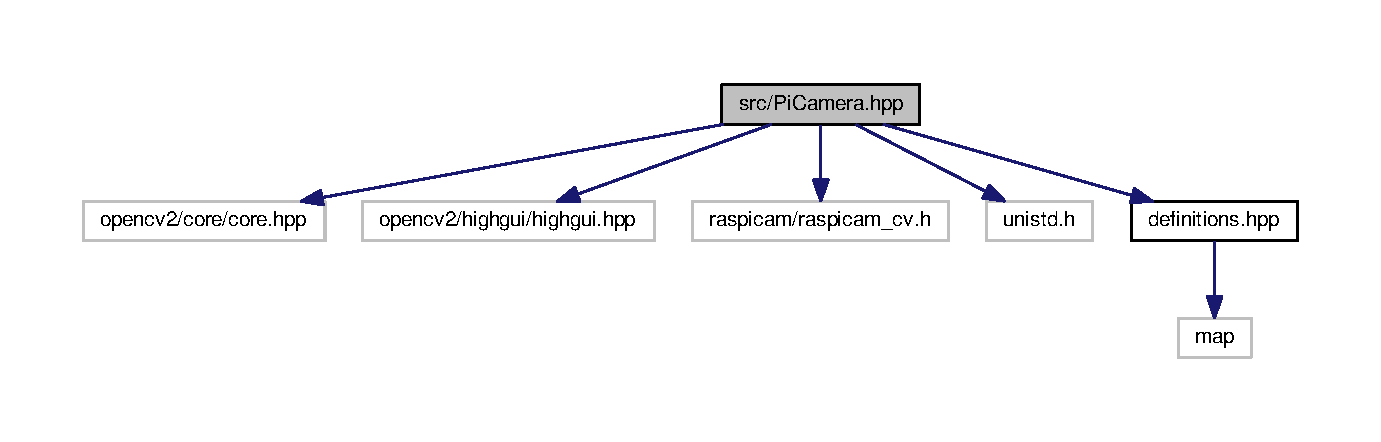
\includegraphics[width=350pt]{PiCamera_8hpp__incl}
\end{center}
\end{figure}
This graph shows which files directly or indirectly include this file\+:
\nopagebreak
\begin{figure}[H]
\begin{center}
\leavevmode
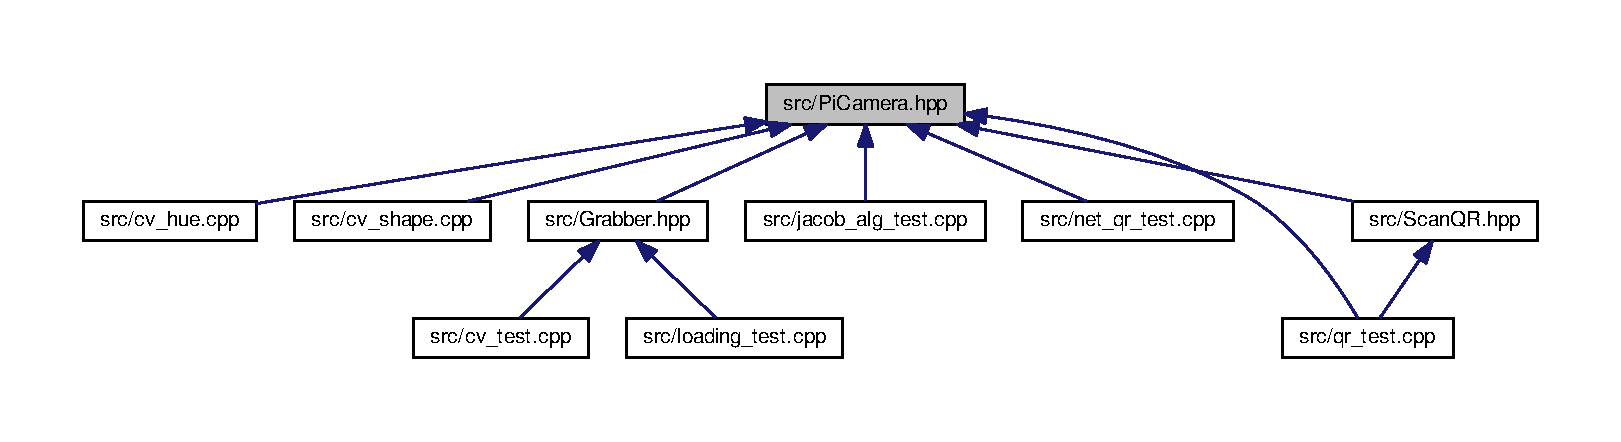
\includegraphics[width=350pt]{PiCamera_8hpp__dep__incl}
\end{center}
\end{figure}
\subsection*{Classes}
\begin{DoxyCompactItemize}
\item 
class \hyperlink{classChipChipArray_1_1PiCamera}{Chip\+Chip\+Array\+::\+Pi\+Camera}
\end{DoxyCompactItemize}
\subsection*{Namespaces}
\begin{DoxyCompactItemize}
\item 
 \hyperlink{namespaceChipChipArray}{Chip\+Chip\+Array}
\end{DoxyCompactItemize}


\subsection{Detailed Description}
Contains Pi\+Camera class. 

\begin{DoxyAuthor}{Author}
Samuel Andrew Wisner, \href{mailto:awisner94@gmail.com}{\tt awisner94@gmail.\+com} 
\end{DoxyAuthor}


Definition in file \hyperlink{PiCamera_8hpp_source}{Pi\+Camera.\+hpp}.


\hypertarget{qr__test_8cpp}{\section{src/qr\+\_\+test.cpp File Reference}
\label{qr__test_8cpp}\index{src/qr\+\_\+test.\+cpp@{src/qr\+\_\+test.\+cpp}}
}


Contains test program for \hyperlink{namespaceChipChipArray_a6c7465049b5d408e1a238b6d8ffa887d}{Scan\+Q\+R()} function.  


{\ttfamily \#include $<$iostream$>$}\\*
{\ttfamily \#include $<$opencv2/core/core.\+hpp$>$}\\*
{\ttfamily \#include $<$opencv2/highgui/highgui.\+hpp$>$}\\*
{\ttfamily \#include $<$string$>$}\\*
{\ttfamily \#include \char`\"{}definitions.\+hpp\char`\"{}}\\*
{\ttfamily \#include \char`\"{}Pi\+Camera.\+hpp\char`\"{}}\\*
{\ttfamily \#include \char`\"{}Scan\+Q\+R.\+hpp\char`\"{}}\\*
Include dependency graph for qr\+\_\+test.\+cpp\+:
\nopagebreak
\begin{figure}[H]
\begin{center}
\leavevmode
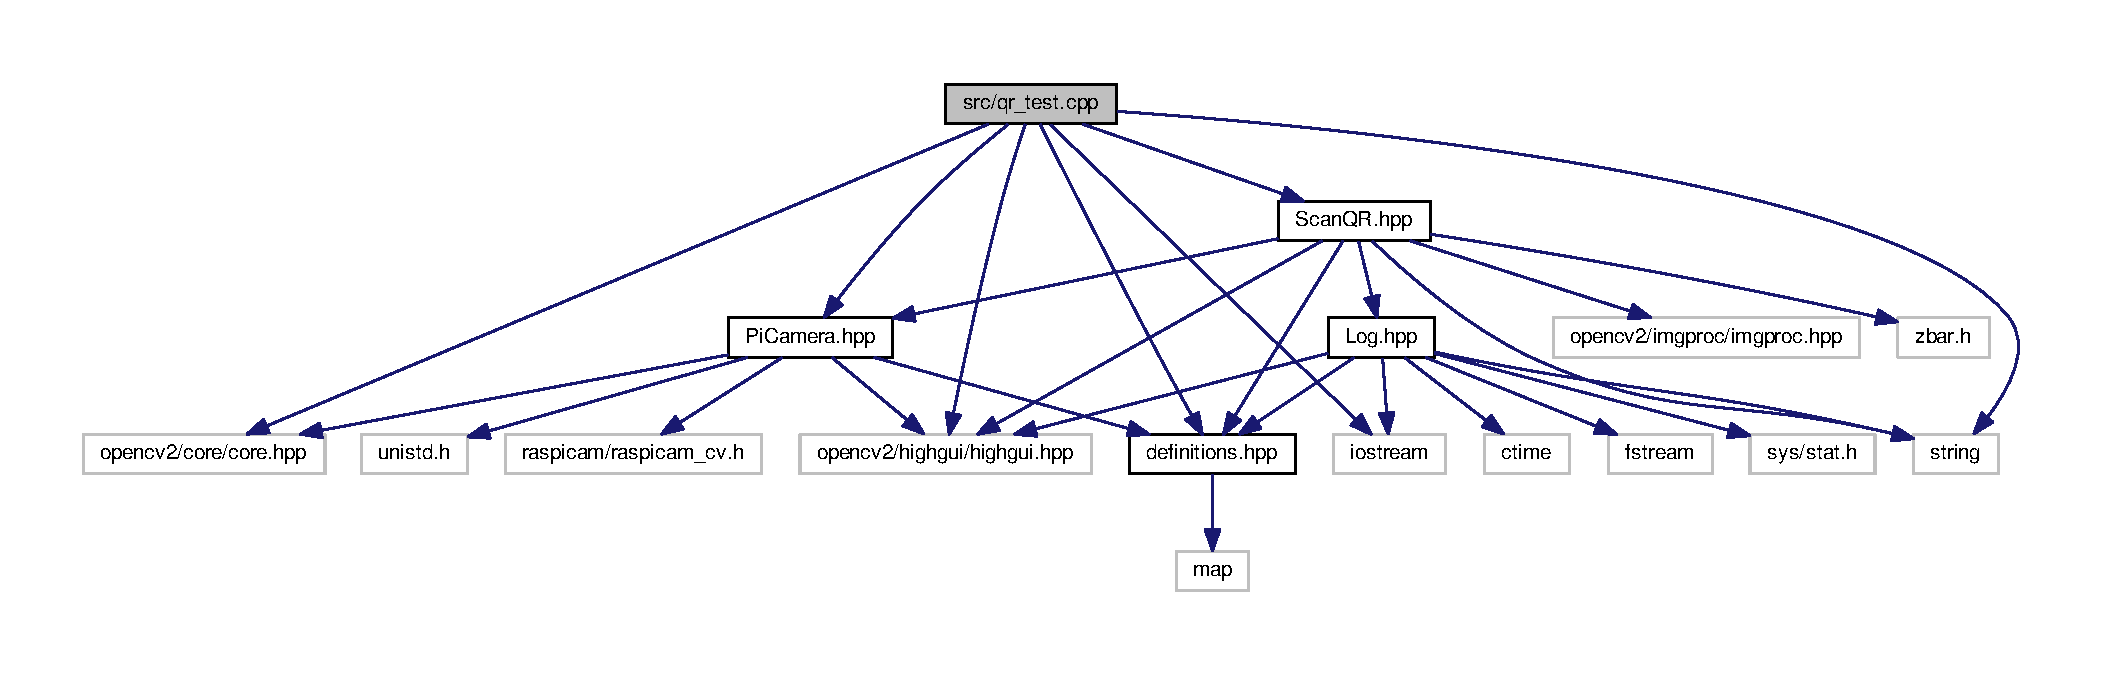
\includegraphics[width=350pt]{qr__test_8cpp__incl}
\end{center}
\end{figure}
\subsection*{Functions}
\begin{DoxyCompactItemize}
\item 
int \hyperlink{qr__test_8cpp_ae66f6b31b5ad750f1fe042a706a4e3d4}{main} ()
\end{DoxyCompactItemize}


\subsection{Detailed Description}
Contains test program for \hyperlink{namespaceChipChipArray_a6c7465049b5d408e1a238b6d8ffa887d}{Scan\+Q\+R()} function. 

\begin{DoxyAuthor}{Author}
Samuel Andrew Wisner, \href{mailto:awisner94@gmail.com}{\tt awisner94@gmail.\+com} 
\end{DoxyAuthor}


Definition in file \hyperlink{qr__test_8cpp_source}{qr\+\_\+test.\+cpp}.



\subsection{Function Documentation}
\hypertarget{qr__test_8cpp_ae66f6b31b5ad750f1fe042a706a4e3d4}{\index{qr\+\_\+test.\+cpp@{qr\+\_\+test.\+cpp}!main@{main}}
\index{main@{main}!qr\+\_\+test.\+cpp@{qr\+\_\+test.\+cpp}}
\subsubsection[{main}]{\setlength{\rightskip}{0pt plus 5cm}int main (
\begin{DoxyParamCaption}
{}
\end{DoxyParamCaption}
)}}\label{qr__test_8cpp_ae66f6b31b5ad750f1fe042a706a4e3d4}
This program tests the \hyperlink{namespaceChipChipArray_a6c7465049b5d408e1a238b6d8ffa887d}{Scan\+Q\+R()} function in terms of reading Q\+R codes (not moving the arm). 

Definition at line \hyperlink{qr__test_8cpp_source_l00022}{22} of file \hyperlink{qr__test_8cpp_source}{qr\+\_\+test.\+cpp}.


\begin{DoxyCode}
00022            \{
00023     \textcolor{keywordflow}{while}(\textcolor{keyword}{true}) \{
00024         \hyperlink{definitions_8hpp_abc05a0f46084a3477cf5d5c939ff1436}{Color} color = \hyperlink{namespaceChipChipArray_a6c7465049b5d408e1a238b6d8ffa887d}{ScanQR}();
00025         std::string colstr;
00026 
00027         \textcolor{keywordflow}{switch}(color) \{
00028             \textcolor{keywordflow}{case} \hyperlink{definitions_8hpp_abc05a0f46084a3477cf5d5c939ff1436aee38e4d5dd68c4e440825018d549cb47}{Color::Red}:
00029                 colstr = \textcolor{stringliteral}{"RED"};
00030                 \textcolor{keywordflow}{break};
00031 
00032             \textcolor{keywordflow}{case} \hyperlink{definitions_8hpp_abc05a0f46084a3477cf5d5c939ff1436a51e6cd92b6c45f9affdc158ecca2b8b8}{Color::Yellow}:
00033                 colstr = \textcolor{stringliteral}{"YELLOW"};
00034                 \textcolor{keywordflow}{break};
00035 
00036             \textcolor{keywordflow}{case} \hyperlink{definitions_8hpp_abc05a0f46084a3477cf5d5c939ff1436ad382816a3cbeed082c9e216e7392eed1}{Color::Green}:
00037                 colstr = \textcolor{stringliteral}{"GREEN"};
00038                 \textcolor{keywordflow}{break};
00039 
00040             \textcolor{keywordflow}{case} \hyperlink{definitions_8hpp_abc05a0f46084a3477cf5d5c939ff1436a9594eec95be70e7b1710f730fdda33d9}{Color::Blue}:
00041                 colstr = \textcolor{stringliteral}{"BLUE"};
00042                 \textcolor{keywordflow}{break};
00043 
00044         \}
00045 
00046         std::cout << colstr << std::endl;
00047     \}
00048 \}
\end{DoxyCode}


Here is the call graph for this function\+:
\nopagebreak
\begin{figure}[H]
\begin{center}
\leavevmode
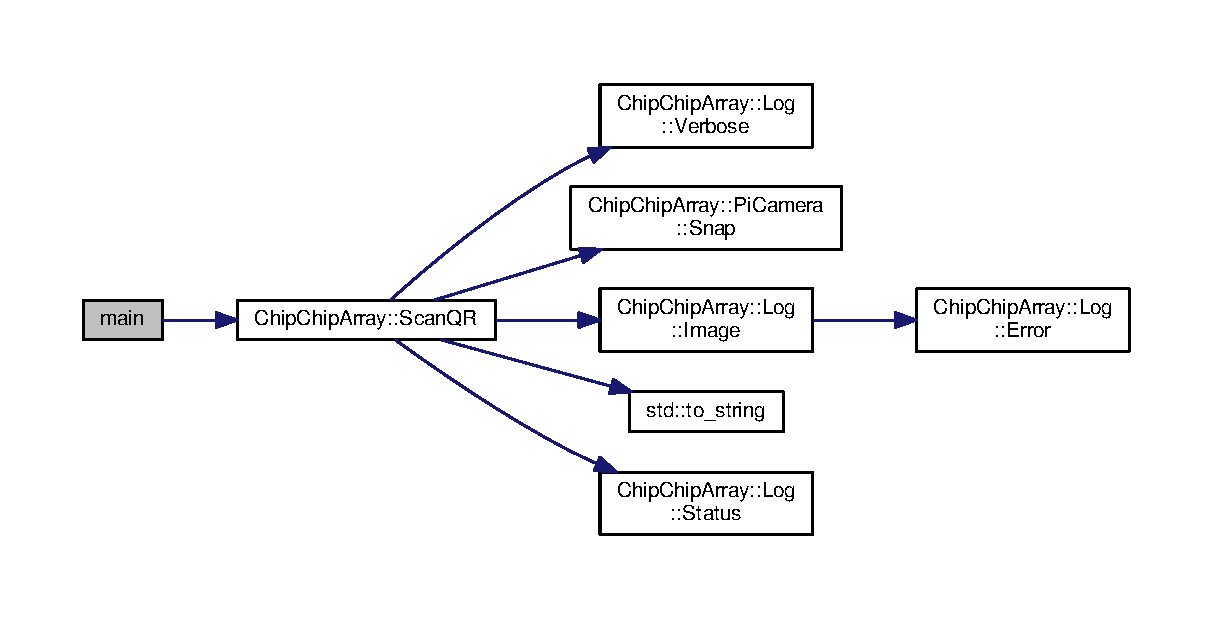
\includegraphics[width=350pt]{qr__test_8cpp_ae66f6b31b5ad750f1fe042a706a4e3d4_cgraph}
\end{center}
\end{figure}



\hypertarget{ScanQR_8hpp}{\section{src/\+Scan\+Q\+R.hpp File Reference}
\label{ScanQR_8hpp}\index{src/\+Scan\+Q\+R.\+hpp@{src/\+Scan\+Q\+R.\+hpp}}
}
{\ttfamily \#include $<$string$>$}\\*
{\ttfamily \#include $<$opencv2/highgui/highgui.\+hpp$>$}\\*
{\ttfamily \#include $<$opencv2/imgproc/imgproc.\+hpp$>$}\\*
{\ttfamily \#include $<$zbar.\+h$>$}\\*
{\ttfamily \#include \char`\"{}definitions.\+hpp\char`\"{}}\\*
{\ttfamily \#include \char`\"{}Pi\+Camera.\+hpp\char`\"{}}\\*
Include dependency graph for Scan\+Q\+R.\+hpp\+:
This graph shows which files directly or indirectly include this file\+:
\subsection*{Namespaces}
\begin{DoxyCompactItemize}
\item 
 \hyperlink{namespaceChipChipArray}{Chip\+Chip\+Array}
\end{DoxyCompactItemize}
\subsection*{Functions}
\begin{DoxyCompactItemize}
\item 
\hyperlink{definitions_8hpp_abc05a0f46084a3477cf5d5c939ff1436}{Color} \hyperlink{namespaceChipChipArray_a6c7465049b5d408e1a238b6d8ffa887d}{Chip\+Chip\+Array\+::\+Scan\+Q\+R} ()
\end{DoxyCompactItemize}

\hypertarget{Servo__Position__Shell_8cpp}{\section{src/\+Servo\+\_\+\+Position\+\_\+\+Shell.cpp File Reference}
\label{Servo__Position__Shell_8cpp}\index{src/\+Servo\+\_\+\+Position\+\_\+\+Shell.\+cpp@{src/\+Servo\+\_\+\+Position\+\_\+\+Shell.\+cpp}}
}


C\+Ontains the function definitions for the servo position shell.  


{\ttfamily \#include $<$wiring\+Pi.\+h$>$}\\*
{\ttfamily \#include \char`\"{}Adafruit\+\_\+\+P\+W\+M\+Servo\+Driver.\+cpp\char`\"{}}\\*
{\ttfamily \#include $<$iostream$>$}\\*
{\ttfamily \#include \char`\"{}Servo\+\_\+\+Position\+\_\+\+Shell.\+h\char`\"{}}\\*
Include dependency graph for Servo\+\_\+\+Position\+\_\+\+Shell.\+cpp\+:
\nopagebreak
\begin{figure}[H]
\begin{center}
\leavevmode
\includegraphics[width=350pt]{Servo__Position__Shell_8cpp__incl}
\end{center}
\end{figure}
This graph shows which files directly or indirectly include this file\+:
\nopagebreak
\begin{figure}[H]
\begin{center}
\leavevmode
\includegraphics[width=333pt]{Servo__Position__Shell_8cpp__dep__incl}
\end{center}
\end{figure}
\subsection*{Macros}
\begin{DoxyCompactItemize}
\item 
\#define \hyperlink{Servo__Position__Shell_8cpp_a65ff49a6e78be84de6e478345b32b508}{S\+E\+R\+V\+O\+M\+I\+N}~150
\item 
\#define \hyperlink{Servo__Position__Shell_8cpp_a357a7e9fa4e4d8ed2f5ef82f37143836}{S\+E\+R\+V\+O\+M\+A\+X}~600
\end{DoxyCompactItemize}
\subsection*{Functions}
\begin{DoxyCompactItemize}
\item 
void \hyperlink{Servo__Position__Shell_8cpp_a4fc01d736fe50cf5b977f755b675f11d}{setup} ()
\item 
void \hyperlink{Servo__Position__Shell_8cpp_a7f07c548295f3696f8881f0c9de708b1}{set\+Servo\+Pulse} (\hyperlink{NavigationControl_8h_ab077fa1127453be2bd9d4c3c8a768fa7}{uint8\+\_\+t} \hyperlink{Servo__Position__Shell_8cpp_ac3fe65cfcd6744437ab3133c702ade33}{servo\+\_\+num}, double pulse)
\item 
void \hyperlink{Servo__Position__Shell_8cpp_abd2cd3c2e36d42a2178a6f2fd12af905}{set\+Servo\+Position} (\hyperlink{Servo__Position__Shell_8h_af629c4ae98db77091b130c7fbc31cab2}{Servo} whichservo, int position)
\end{DoxyCompactItemize}
\subsection*{Variables}
\begin{DoxyCompactItemize}
\item 
\hyperlink{classAdafruit__PWMServoDriver}{Adafruit\+\_\+\+P\+W\+M\+Servo\+Driver} \hyperlink{Servo__Position__Shell_8cpp_a2c06cc8f85429bb0f7cb91917164dc54}{pwm} = \hyperlink{classAdafruit__PWMServoDriver}{Adafruit\+\_\+\+P\+W\+M\+Servo\+Driver}()
\item 
\hyperlink{NavigationControl_8h_ab077fa1127453be2bd9d4c3c8a768fa7}{uint8\+\_\+t} \hyperlink{Servo__Position__Shell_8cpp_ac3fe65cfcd6744437ab3133c702ade33}{servo\+\_\+num}
\end{DoxyCompactItemize}


\subsection{Detailed Description}
C\+Ontains the function definitions for the servo position shell. 

\begin{DoxyAuthor}{Author}
Nickolas Neely 
\end{DoxyAuthor}
\begin{DoxyDate}{Date}
8. February 2016, 12\+:05 P\+M 
\end{DoxyDate}


Definition in file \hyperlink{Servo__Position__Shell_8cpp_source}{Servo\+\_\+\+Position\+\_\+\+Shell.\+cpp}.



\subsection{Macro Definition Documentation}
\hypertarget{Servo__Position__Shell_8cpp_a357a7e9fa4e4d8ed2f5ef82f37143836}{\index{Servo\+\_\+\+Position\+\_\+\+Shell.\+cpp@{Servo\+\_\+\+Position\+\_\+\+Shell.\+cpp}!S\+E\+R\+V\+O\+M\+A\+X@{S\+E\+R\+V\+O\+M\+A\+X}}
\index{S\+E\+R\+V\+O\+M\+A\+X@{S\+E\+R\+V\+O\+M\+A\+X}!Servo\+\_\+\+Position\+\_\+\+Shell.\+cpp@{Servo\+\_\+\+Position\+\_\+\+Shell.\+cpp}}
\subsubsection[{S\+E\+R\+V\+O\+M\+A\+X}]{\setlength{\rightskip}{0pt plus 5cm}\#define S\+E\+R\+V\+O\+M\+A\+X~600}}\label{Servo__Position__Shell_8cpp_a357a7e9fa4e4d8ed2f5ef82f37143836}


Definition at line \hyperlink{Servo__Position__Shell_8cpp_source_l00031}{31} of file \hyperlink{Servo__Position__Shell_8cpp_source}{Servo\+\_\+\+Position\+\_\+\+Shell.\+cpp}.

\hypertarget{Servo__Position__Shell_8cpp_a65ff49a6e78be84de6e478345b32b508}{\index{Servo\+\_\+\+Position\+\_\+\+Shell.\+cpp@{Servo\+\_\+\+Position\+\_\+\+Shell.\+cpp}!S\+E\+R\+V\+O\+M\+I\+N@{S\+E\+R\+V\+O\+M\+I\+N}}
\index{S\+E\+R\+V\+O\+M\+I\+N@{S\+E\+R\+V\+O\+M\+I\+N}!Servo\+\_\+\+Position\+\_\+\+Shell.\+cpp@{Servo\+\_\+\+Position\+\_\+\+Shell.\+cpp}}
\subsubsection[{S\+E\+R\+V\+O\+M\+I\+N}]{\setlength{\rightskip}{0pt plus 5cm}\#define S\+E\+R\+V\+O\+M\+I\+N~150}}\label{Servo__Position__Shell_8cpp_a65ff49a6e78be84de6e478345b32b508}


Definition at line \hyperlink{Servo__Position__Shell_8cpp_source_l00030}{30} of file \hyperlink{Servo__Position__Shell_8cpp_source}{Servo\+\_\+\+Position\+\_\+\+Shell.\+cpp}.



\subsection{Function Documentation}
\hypertarget{Servo__Position__Shell_8cpp_abd2cd3c2e36d42a2178a6f2fd12af905}{\index{Servo\+\_\+\+Position\+\_\+\+Shell.\+cpp@{Servo\+\_\+\+Position\+\_\+\+Shell.\+cpp}!set\+Servo\+Position@{set\+Servo\+Position}}
\index{set\+Servo\+Position@{set\+Servo\+Position}!Servo\+\_\+\+Position\+\_\+\+Shell.\+cpp@{Servo\+\_\+\+Position\+\_\+\+Shell.\+cpp}}
\subsubsection[{set\+Servo\+Position}]{\setlength{\rightskip}{0pt plus 5cm}void set\+Servo\+Position (
\begin{DoxyParamCaption}
\item[{{\bf Servo}}]{whichservo, }
\item[{int}]{position}
\end{DoxyParamCaption}
)}}\label{Servo__Position__Shell_8cpp_abd2cd3c2e36d42a2178a6f2fd12af905}
Desc\+: This function sets which servo to use using whichservo and what position out of 180 degrees for each servo (with limits). 
\begin{DoxyParams}{Parameters}
{\em whichservo} & which servo would you like to use on the board \\
\hline
{\em position} & what position do you want to set the servo selected at \\
\hline
\end{DoxyParams}


Definition at line \hyperlink{Servo__Position__Shell_8cpp_source_l00071}{71} of file \hyperlink{Servo__Position__Shell_8cpp_source}{Servo\+\_\+\+Position\+\_\+\+Shell.\+cpp}.


\begin{DoxyCode}
00071                                                       \{
00072     \textcolor{comment}{// works for servo 0, 3, 4}
00073     \textcolor{keywordtype}{double} dividedconstant = 180.0;
00074     \textcolor{keywordtype}{double} highservo = 2.4;
00075     \textcolor{keywordtype}{double} lowservo = 0.6;
00076     \textcolor{comment}{// To fix the magical digital servo on LIFT 1}
00077     \textcolor{keywordtype}{double} highservoweird = 1.9;
00078     \textcolor{keywordtype}{double} lowservoweird = 0.6;
00079     \textcolor{comment}{// To compensate for the bent servo spline on LIFT 2}
00080     \textcolor{keywordtype}{double} highservospline = 2.25;
00081     \textcolor{keywordtype}{double} lowservospline = 0.6;
00082     \textcolor{comment}{// works for servo 1, 2}
00083     \textcolor{keywordtype}{double} digitalservohigh = 2.45;
00084     \textcolor{keywordtype}{double} digitalservolow = 0.9;
00085     \textcolor{comment}{// left gripper servo 5}
00086     \textcolor{keywordtype}{double} gripleftopen = 2.2;
00087     \textcolor{keywordtype}{double} gripleftclose = 1.3;
00088     \textcolor{comment}{// right gripper servo 6}
00089     \textcolor{keywordtype}{double} griprightopen = 2.2;
00090     \textcolor{keywordtype}{double} griprightclose = 1.3;
00091     \textcolor{keywordtype}{double} pulse;
00092 
00093     \textcolor{keywordflow}{switch} (whichservo) \{
00094 
00095             \textcolor{comment}{// BASE TURN}
00096         \textcolor{keywordflow}{case} 0:
00097         \{
00098             \textcolor{keywordflow}{if} (position == -1) \{
00099                 pulse = 0.0;
00100             \}\textcolor{keywordflow}{else} \textcolor{keywordflow}{if} (position < 0)\{
00101                 position = 20;
00102                 pulse = ((((highservo - lowservo) / dividedconstant)*((double) position)) + lowservo);
00103             \}\textcolor{keywordflow}{else} \textcolor{keywordflow}{if} (position > 179)\{
00104                 position = 179;
00105                 pulse = ((((highservo - lowservo) / dividedconstant)*((double) position)) + lowservo);
00106             \}\textcolor{keywordflow}{else}\{
00107                 pulse = ((((highservo - lowservo) / dividedconstant)*((double) position)) + lowservo);
00108             \}
00109             
00110         \}
00111 
00112             \textcolor{keywordflow}{break};
00113 
00114             \textcolor{comment}{// BASE TILT}
00115         \textcolor{keywordflow}{case} 1:
00116         \{
00117             
00118             
00119             \textcolor{keywordflow}{if} (position == -1) \{
00120                 pulse = 0.0;
00121             \} \textcolor{keywordflow}{else} \textcolor{keywordflow}{if} (position < 90)\{
00122                 position = 90;
00123                 pulse = ((((highservo - lowservo) / dividedconstant)*((double) position)) + lowservo);
00124             \} \textcolor{keywordflow}{else} \textcolor{keywordflow}{if} (position > 172)\{
00125                 position = 172;
00126                 pulse = ((((highservo - lowservo) / dividedconstant)*((double) position)) + lowservo);
00127             \} \textcolor{keywordflow}{else} \{
00128                 pulse = ((((highservo - lowservo) / dividedconstant)*((double) position)) + lowservo);
00129             \}
00130         \}
00131             \textcolor{keywordflow}{break};
00132 
00133             \textcolor{comment}{// ELBOW}
00134         \textcolor{keywordflow}{case} 2:
00135         \{
00136             \textcolor{keywordflow}{if} (position == -1) \{
00137                 pulse = 0.0;
00138             \} \textcolor{keywordflow}{else} \textcolor{keywordflow}{if} (position < 43)\{
00139                 position = 43;
00140                 pulse = ((((digitalservohigh - digitalservolow) / dividedconstant)*((double) position)) + 
      digitalservolow);
00141             \} \textcolor{keywordflow}{else} \textcolor{keywordflow}{if} (position > 179)\{
00142                 position = 179;
00143                 pulse = ((((digitalservohigh - digitalservolow) / dividedconstant)*((double) position)) + 
      digitalservolow);
00144             \} \textcolor{keywordflow}{else} \{
00145                 pulse = ((((digitalservohigh - digitalservolow) / dividedconstant)*((double) position)) + 
      digitalservolow);
00146             \}
00147         \}
00148             \textcolor{keywordflow}{break};
00149 
00150             \textcolor{comment}{// WRIST TURN}
00151         \textcolor{keywordflow}{case} 3:
00152         \{
00153             \textcolor{keywordflow}{if} (position == -1) \{
00154                 pulse = 0.0;
00155             \} \textcolor{keywordflow}{else} \{
00156                 pulse = ((((highservo - lowservo) / dividedconstant)*((double) position)) + lowservo);
00157             \}
00158         \}
00159             \textcolor{keywordflow}{break};
00160 
00161             \textcolor{comment}{// WRIST PAN}
00162         \textcolor{keywordflow}{case} 4:
00163         \{
00164             \textcolor{keywordflow}{if} (position == -1) \{
00165                 pulse = 0.0;
00166             \} \textcolor{keywordflow}{else} \textcolor{keywordflow}{if} (position < 0)\{
00167                 position = 0;
00168                 pulse = ((((highservo - lowservo) / dividedconstant)*((double) position)) + lowservo);
00169             \} \textcolor{keywordflow}{else} \textcolor{keywordflow}{if} (position > 180)\{
00170                 position = 180;
00171                 pulse = ((((highservo - lowservo) / dividedconstant)*((double) position)) + lowservo);
00172             \} \textcolor{keywordflow}{else} \{
00173                 pulse = ((((highservo - lowservo) / dividedconstant)*((double) position)) + lowservo);
00174             \}
00175         \}
00176             \textcolor{keywordflow}{break};
00177 
00178             \textcolor{comment}{// GRIP LEFT}
00179         \textcolor{keywordflow}{case} 5:
00180         \{
00181             \textcolor{keywordflow}{if} (position == -1) \{
00182                 pulse = 0.0;
00183             \} \textcolor{keywordflow}{else} \textcolor{keywordflow}{if}(position < 0)\{
00184                 position = 0;
00185                 pulse = ((((griprightopen - griprightclose) / dividedconstant)*((double) position)) + 
      griprightclose);
00186             \}\textcolor{keywordflow}{else} \textcolor{keywordflow}{if}(position > 90)\{
00187                 position = 90;
00188                 pulse = ((((griprightopen - griprightclose) / dividedconstant)*((double) position)) + 
      griprightclose);
00189             \} \textcolor{keywordflow}{else} \{
00190                 pulse = ((((gripleftopen - gripleftclose) / dividedconstant)*((double) position)) + 
      gripleftclose);
00191             \}
00192         \}
00193             \textcolor{keywordflow}{break};
00194 
00195             \textcolor{comment}{// GRIP RIGHT}
00196         \textcolor{keywordflow}{case} 6:
00197         \{
00198             \textcolor{keywordflow}{if} (position == -1) \{
00199                 pulse = 0.0;
00200             \} \textcolor{keywordflow}{else} \textcolor{keywordflow}{if}(position < 90)\{
00201                 position = 90;
00202                 pulse = ((((griprightopen - griprightclose) / dividedconstant)*((double) position)) + 
      griprightclose);
00203             \} \textcolor{keywordflow}{else} \textcolor{keywordflow}{if}(position > 180)\{
00204                 position = 180;
00205                 pulse = ((((griprightopen - griprightclose) / dividedconstant)*((double) position)) + 
      griprightclose);
00206             \}\textcolor{keywordflow}{else}\{
00207                 pulse = ((((griprightopen - griprightclose) / dividedconstant)*((double) position)) + 
      griprightclose);
00208             \}
00209         \}
00210             \textcolor{keywordflow}{break};
00211 
00212             \textcolor{comment}{// Michael Yellow Gate}
00213         \textcolor{keywordflow}{case} 7:
00214         \{
00215             \textcolor{keywordflow}{if} (position == -1) \{
00216                 pulse = 0.0;
00217             \} \textcolor{keywordflow}{else} \textcolor{keywordflow}{if}(position < 0)\{
00218                 position = 0;
00219                 pulse = ((((highservo - lowservo) / dividedconstant)*((double) position)) + lowservo);
00220             \} \textcolor{keywordflow}{else} \textcolor{keywordflow}{if}(position > 90)\{
00221                 position = 90;
00222                 pulse = ((((highservo - lowservo) / dividedconstant)*((double) position)) + lowservo);
00223             \} \textcolor{keywordflow}{else} \{
00224                 pulse = ((((highservo - lowservo) / dividedconstant)*((double) position)) + lowservo);
00225             \}
00226         \}
00227             \textcolor{keywordflow}{break};
00228 
00229             \textcolor{comment}{// Michael Green Gate}
00230         \textcolor{keywordflow}{case} 8:
00231         \{
00232             \textcolor{keywordflow}{if} (position == -1) \{
00233                 pulse = 0.0;
00234             \} \textcolor{keywordflow}{else} \textcolor{keywordflow}{if}(position < 0)\{
00235                 position = 0;
00236                 pulse = ((((highservo - lowservo) / dividedconstant)*((double) position)) + lowservo);
00237             \} \textcolor{keywordflow}{else} \textcolor{keywordflow}{if}(position > 90)\{
00238                 position = 90;
00239                 pulse = ((((highservo - lowservo) / dividedconstant)*((double) position)) + lowservo);
00240             \} \textcolor{keywordflow}{else} \{
00241                 pulse = ((((highservo - lowservo) / dividedconstant)*((double) position)) + lowservo);
00242             \}
00243         \}
00244             \textcolor{keywordflow}{break};
00245 
00246             \textcolor{comment}{// Michael Blue Gate}
00247         \textcolor{keywordflow}{case} 9:
00248         \{
00249             \textcolor{keywordflow}{if} (position == -1) \{
00250                 pulse = 0.0;
00251             \} \textcolor{keywordflow}{else} \textcolor{keywordflow}{if}(position < 0)\{
00252                 position = 0;
00253                 pulse = ((((highservo - lowservo) / dividedconstant)*((double) position)) + lowservo);
00254             \} \textcolor{keywordflow}{else} \textcolor{keywordflow}{if}(position > 90)\{
00255                 position = 90;
00256                 pulse = ((((highservo - lowservo) / dividedconstant)*((double) position)) + lowservo);
00257             \} \textcolor{keywordflow}{else} \{
00258                 pulse = ((((highservo - lowservo) / dividedconstant)*((double) position)) + lowservo);
00259             \}
00260         \}
00261             \textcolor{keywordflow}{break};
00262 
00263             \textcolor{comment}{// Michael Lift 1}
00264         \textcolor{keywordflow}{case} 10:
00265         \{
00266             \textcolor{keywordflow}{if} (position == -1) \{
00267                 pulse = 0.0;
00268             \} \textcolor{keywordflow}{else} \textcolor{keywordflow}{if}(position < 0)\{
00269                 position = 0;
00270                 pulse = ((((highservoweird - lowservoweird) / dividedconstant)*((double) position)) + 
      lowservoweird);
00271             \} \textcolor{keywordflow}{else} \textcolor{keywordflow}{if}(position > 105)\{
00272                 position = 105;
00273                 pulse = ((((highservoweird - lowservoweird) / dividedconstant)*((double) position)) + 
      lowservoweird);
00274             \} \textcolor{keywordflow}{else} \{
00275                 pulse = ((((highservoweird - lowservoweird) / dividedconstant)*((double) position)) + 
      lowservoweird);
00276             \}
00277         \}
00278             \textcolor{keywordflow}{break};
00279 
00280             \textcolor{comment}{//Michael Lift 2}
00281         \textcolor{keywordflow}{case} 11:
00282         \{
00283             \textcolor{keywordflow}{if} (position == -1) \{
00284                 pulse = 0.0;
00285             \} \textcolor{keywordflow}{else} \textcolor{keywordflow}{if}(position < 0)\{
00286                 position = 0;
00287                 pulse = ((((highservospline - lowservospline) / dividedconstant)*((double) position)) + 
      lowservospline);
00288             \} \textcolor{keywordflow}{else} \textcolor{keywordflow}{if}(position > 105)\{
00289                 position = 105;
00290                 pulse = ((((highservospline - lowservospline) / dividedconstant)*((double) position)) + 
      lowservospline);
00291             \} \textcolor{keywordflow}{else} \{
00292                 pulse = ((((highservospline - lowservospline) / dividedconstant)*((double) position)) + 
      lowservospline);
00293             \}
00294         \}
00295             \textcolor{keywordflow}{break};
00296 
00297             \textcolor{comment}{//Michael lift 3}
00298         \textcolor{keywordflow}{case} 12:
00299         \{
00300             \textcolor{keywordflow}{if} (position == -1) \{
00301                 pulse = 0.0;
00302             \} \textcolor{keywordflow}{else} \textcolor{keywordflow}{if}(position < 0)\{
00303                 position = 0;
00304                 pulse = ((((highservo - lowservo) / dividedconstant)*((double) position)) + lowservo);
00305             \} \textcolor{keywordflow}{else} \textcolor{keywordflow}{if}(position > 105)\{
00306                 position = 105;
00307                 pulse = ((((highservo - lowservo) / dividedconstant)*((double) position)) + lowservo);
00308             \} \textcolor{keywordflow}{else} \{
00309                 pulse = ((((highservo - lowservo) / dividedconstant)*((double) position)) + lowservo);
00310             \}
00311         \}
00312             \textcolor{keywordflow}{break};
00313 
00314             \textcolor{comment}{// Michael lift 4}
00315         \textcolor{keywordflow}{case} 13:
00316         \{
00317             \textcolor{keywordflow}{if} (position == -1) \{
00318                 pulse = 0.0;
00319             \} \textcolor{keywordflow}{else} \textcolor{keywordflow}{if}(position < 0)\{
00320                 position = 0;
00321                 pulse = ((((highservo - lowservo) / dividedconstant)*((double) position)) + lowservo);
00322             \} \textcolor{keywordflow}{else} \textcolor{keywordflow}{if}(position > 105)\{
00323                 position = 105;
00324                 pulse = ((((highservo - lowservo) / dividedconstant)*((double) position)) + lowservo);
00325             \} \textcolor{keywordflow}{else} \{
00326                 pulse = ((((highservo - lowservo) / dividedconstant)*((double) position)) + lowservo);
00327             \}
00328         \}
00329             \textcolor{keywordflow}{break};
00330 
00331             \textcolor{comment}{// Michael RED GATE}
00332         \textcolor{keywordflow}{case} 14:
00333         \{
00334             \textcolor{keywordflow}{if} (position == -1) \{
00335                 pulse = 0.0;
00336             \} \textcolor{keywordflow}{else} \textcolor{keywordflow}{if}(position < 0)\{
00337                 position = 0;
00338                 pulse = ((((highservo - lowservo) / dividedconstant)*((double) position)) + lowservo);
00339             \} \textcolor{keywordflow}{else} \textcolor{keywordflow}{if}(position > 105)\{
00340                 position = 105;
00341                 pulse = ((((highservo - lowservo) / dividedconstant)*((double) position)) + lowservo);
00342             \} \textcolor{keywordflow}{else} \{
00343                 pulse = ((((highservo - lowservo) / dividedconstant)*((double) position)) + lowservo);
00344             \}
00345         \}
00346             \textcolor{keywordflow}{break};
00347     \}
00348     \hyperlink{Servo__Position__Shell_8cpp_a7f07c548295f3696f8881f0c9de708b1}{setServoPulse}(whichservo, pulse);
00349 
00350 \}
\end{DoxyCode}


Here is the call graph for this function\+:
\nopagebreak
\begin{figure}[H]
\begin{center}
\leavevmode
\includegraphics[width=350pt]{Servo__Position__Shell_8cpp_abd2cd3c2e36d42a2178a6f2fd12af905_cgraph}
\end{center}
\end{figure}




Here is the caller graph for this function\+:
\nopagebreak
\begin{figure}[H]
\begin{center}
\leavevmode
\includegraphics[width=350pt]{Servo__Position__Shell_8cpp_abd2cd3c2e36d42a2178a6f2fd12af905_icgraph}
\end{center}
\end{figure}


\hypertarget{Servo__Position__Shell_8cpp_a7f07c548295f3696f8881f0c9de708b1}{\index{Servo\+\_\+\+Position\+\_\+\+Shell.\+cpp@{Servo\+\_\+\+Position\+\_\+\+Shell.\+cpp}!set\+Servo\+Pulse@{set\+Servo\+Pulse}}
\index{set\+Servo\+Pulse@{set\+Servo\+Pulse}!Servo\+\_\+\+Position\+\_\+\+Shell.\+cpp@{Servo\+\_\+\+Position\+\_\+\+Shell.\+cpp}}
\subsubsection[{set\+Servo\+Pulse}]{\setlength{\rightskip}{0pt plus 5cm}void set\+Servo\+Pulse (
\begin{DoxyParamCaption}
\item[{{\bf uint8\+\_\+t}}]{n, }
\item[{double}]{pulse}
\end{DoxyParamCaption}
)}}\label{Servo__Position__Shell_8cpp_a7f07c548295f3696f8881f0c9de708b1}
Desc\+: This function sets which servo to use and what pulse to set that servos pwm to. 
\begin{DoxyParams}{Parameters}
{\em n} & which servo on the breakout board am I calling. Starting with 0. \\
\hline
{\em pulse} & what is the pulse length (in micro seconds) the pwm of the servo is set to. \\
\hline
\end{DoxyParams}


Definition at line \hyperlink{Servo__Position__Shell_8cpp_source_l00050}{50} of file \hyperlink{Servo__Position__Shell_8cpp_source}{Servo\+\_\+\+Position\+\_\+\+Shell.\+cpp}.


\begin{DoxyCode}
00050                                                     \{
00051     \textcolor{keywordtype}{double} pulselength;
00052 
00053     pulselength = 1000000; \textcolor{comment}{// 1,000,000 us per second}
00054     pulselength /= 60; \textcolor{comment}{// 60 Hz}
00055     \textcolor{comment}{//cout << pulselength << " us per period" << endl;}
00056     pulselength /= 4096; \textcolor{comment}{// 12 bits of resolution}
00057     \textcolor{comment}{//cout << pulselength << "us per bit" << endl;}
00058     pulse *= 1000;
00059     pulse /= pulselength;
00060     \textcolor{comment}{//cout << (uint16\_t) pulse << endl;}
00061     \hyperlink{Servo__Position__Shell_8cpp_a2c06cc8f85429bb0f7cb91917164dc54}{pwm}.\hyperlink{classAdafruit__PWMServoDriver_a724a7fc39c6fba34478ecc0eea038bd3}{setPWM}(\hyperlink{Servo__Position__Shell_8cpp_ac3fe65cfcd6744437ab3133c702ade33}{servo\_num}, 0, (\hyperlink{Adafruit__PWMServoDriver_8h_a395b3b2bf5cb4674ab41b6bda68c15bb}{uint16\_t}) pulse);
00062     \textcolor{comment}{//cout << endl;}
00063 \}
\end{DoxyCode}


Here is the call graph for this function\+:
\nopagebreak
\begin{figure}[H]
\begin{center}
\leavevmode
\includegraphics[width=328pt]{Servo__Position__Shell_8cpp_a7f07c548295f3696f8881f0c9de708b1_cgraph}
\end{center}
\end{figure}




Here is the caller graph for this function\+:
\nopagebreak
\begin{figure}[H]
\begin{center}
\leavevmode
\includegraphics[width=350pt]{Servo__Position__Shell_8cpp_a7f07c548295f3696f8881f0c9de708b1_icgraph}
\end{center}
\end{figure}


\hypertarget{Servo__Position__Shell_8cpp_a4fc01d736fe50cf5b977f755b675f11d}{\index{Servo\+\_\+\+Position\+\_\+\+Shell.\+cpp@{Servo\+\_\+\+Position\+\_\+\+Shell.\+cpp}!setup@{setup}}
\index{setup@{setup}!Servo\+\_\+\+Position\+\_\+\+Shell.\+cpp@{Servo\+\_\+\+Position\+\_\+\+Shell.\+cpp}}
\subsubsection[{setup}]{\setlength{\rightskip}{0pt plus 5cm}void setup (
\begin{DoxyParamCaption}
{}
\end{DoxyParamCaption}
)}}\label{Servo__Position__Shell_8cpp_a4fc01d736fe50cf5b977f755b675f11d}
Desc\+: This function sets up the breakout board communication with I2\+C using Adafruits\+\_\+\+P\+W\+M\+Servo\+Driver.\+cpp and to set the frequency of the servos to 60\+Hz. 

Definition at line \hyperlink{Servo__Position__Shell_8cpp_source_l00041}{41} of file \hyperlink{Servo__Position__Shell_8cpp_source}{Servo\+\_\+\+Position\+\_\+\+Shell.\+cpp}.


\begin{DoxyCode}
00041              \{
00042     \textcolor{comment}{//cout << "Testing Servos" << endl;}
00043     \hyperlink{Servo__Position__Shell_8cpp_a2c06cc8f85429bb0f7cb91917164dc54}{pwm}.\hyperlink{classAdafruit__PWMServoDriver_aef401eaad3c34222ac916eb7bd936bc2}{begin}();
00044     \hyperlink{Servo__Position__Shell_8cpp_a2c06cc8f85429bb0f7cb91917164dc54}{pwm}.\hyperlink{classAdafruit__PWMServoDriver_a0ef6f1e3c81aebbd1d1da1bb12f3ed5c}{setPWMFreq}(60.0); \textcolor{comment}{// Analog servos run at ~60 Hz updates}
00045 \}
\end{DoxyCode}


Here is the call graph for this function\+:
\nopagebreak
\begin{figure}[H]
\begin{center}
\leavevmode
\includegraphics[width=350pt]{Servo__Position__Shell_8cpp_a4fc01d736fe50cf5b977f755b675f11d_cgraph}
\end{center}
\end{figure}




Here is the caller graph for this function\+:
\nopagebreak
\begin{figure}[H]
\begin{center}
\leavevmode
\includegraphics[width=285pt]{Servo__Position__Shell_8cpp_a4fc01d736fe50cf5b977f755b675f11d_icgraph}
\end{center}
\end{figure}




\subsection{Variable Documentation}
\hypertarget{Servo__Position__Shell_8cpp_a2c06cc8f85429bb0f7cb91917164dc54}{\index{Servo\+\_\+\+Position\+\_\+\+Shell.\+cpp@{Servo\+\_\+\+Position\+\_\+\+Shell.\+cpp}!pwm@{pwm}}
\index{pwm@{pwm}!Servo\+\_\+\+Position\+\_\+\+Shell.\+cpp@{Servo\+\_\+\+Position\+\_\+\+Shell.\+cpp}}
\subsubsection[{pwm}]{\setlength{\rightskip}{0pt plus 5cm}{\bf Adafruit\+\_\+\+P\+W\+M\+Servo\+Driver} pwm = {\bf Adafruit\+\_\+\+P\+W\+M\+Servo\+Driver}()}}\label{Servo__Position__Shell_8cpp_a2c06cc8f85429bb0f7cb91917164dc54}


Definition at line \hyperlink{Servo__Position__Shell_8cpp_source_l00022}{22} of file \hyperlink{Servo__Position__Shell_8cpp_source}{Servo\+\_\+\+Position\+\_\+\+Shell.\+cpp}.

\hypertarget{Servo__Position__Shell_8cpp_ac3fe65cfcd6744437ab3133c702ade33}{\index{Servo\+\_\+\+Position\+\_\+\+Shell.\+cpp@{Servo\+\_\+\+Position\+\_\+\+Shell.\+cpp}!servo\+\_\+num@{servo\+\_\+num}}
\index{servo\+\_\+num@{servo\+\_\+num}!Servo\+\_\+\+Position\+\_\+\+Shell.\+cpp@{Servo\+\_\+\+Position\+\_\+\+Shell.\+cpp}}
\subsubsection[{servo\+\_\+num}]{\setlength{\rightskip}{0pt plus 5cm}{\bf uint8\+\_\+t} servo\+\_\+num}}\label{Servo__Position__Shell_8cpp_ac3fe65cfcd6744437ab3133c702ade33}


Definition at line \hyperlink{Servo__Position__Shell_8cpp_source_l00034}{34} of file \hyperlink{Servo__Position__Shell_8cpp_source}{Servo\+\_\+\+Position\+\_\+\+Shell.\+cpp}.


\hypertarget{Servo__Position__Shell_8h}{\section{src/\+Servo\+\_\+\+Position\+\_\+\+Shell.h File Reference}
\label{Servo__Position__Shell_8h}\index{src/\+Servo\+\_\+\+Position\+\_\+\+Shell.\+h@{src/\+Servo\+\_\+\+Position\+\_\+\+Shell.\+h}}
}


Contains the function prototypes for the servo position shell.  


{\ttfamily \#include $<$wiring\+Pi.\+h$>$}\\*
{\ttfamily \#include \char`\"{}Adafruit\+\_\+\+P\+W\+M\+Servo\+Driver.\+h\char`\"{}}\\*
{\ttfamily \#include $<$iostream$>$}\\*
{\ttfamily \#include $<$ctype.\+h$>$}\\*
{\ttfamily \#include $<$cstdint$>$}\\*
Include dependency graph for Servo\+\_\+\+Position\+\_\+\+Shell.\+h\+:
\nopagebreak
\begin{figure}[H]
\begin{center}
\leavevmode
\includegraphics[width=350pt]{Servo__Position__Shell_8h__incl}
\end{center}
\end{figure}
This graph shows which files directly or indirectly include this file\+:
\nopagebreak
\begin{figure}[H]
\begin{center}
\leavevmode
\includegraphics[width=350pt]{Servo__Position__Shell_8h__dep__incl}
\end{center}
\end{figure}
\subsection*{Enumerations}
\begin{DoxyCompactItemize}
\item 
enum \hyperlink{Servo__Position__Shell_8h_af629c4ae98db77091b130c7fbc31cab2}{Servo} \{ \\*
\hyperlink{Servo__Position__Shell_8h_af629c4ae98db77091b130c7fbc31cab2a87afce59ad3a309ba92f43778dde0edf}{B\+A\+S\+E\+\_\+\+T\+U\+R\+N} = 0, 
\hyperlink{Servo__Position__Shell_8h_af629c4ae98db77091b130c7fbc31cab2a793d7330231df1a295a841e5b2bb9a8c}{B\+A\+S\+E\+\_\+\+T\+I\+L\+T} = 1, 
\hyperlink{Servo__Position__Shell_8h_af629c4ae98db77091b130c7fbc31cab2a9b1c0cf4eb53d13971a120133cf44232}{E\+L\+B\+O\+W} = 2, 
\hyperlink{Servo__Position__Shell_8h_af629c4ae98db77091b130c7fbc31cab2abb1046e4dfca68924f935e255b6fae54}{W\+R\+I\+S\+T\+\_\+\+T\+I\+L\+T} = 3, 
\\*
\hyperlink{Servo__Position__Shell_8h_af629c4ae98db77091b130c7fbc31cab2a6e375b725a2efd65c7221fd35055d1b6}{W\+R\+I\+S\+T\+\_\+\+P\+A\+N} = 4, 
\hyperlink{Servo__Position__Shell_8h_af629c4ae98db77091b130c7fbc31cab2a084d4bf780fc2715f33c1f33387c3c76}{G\+R\+I\+P\+\_\+\+R\+I\+G\+H\+T} = 5, 
\hyperlink{Servo__Position__Shell_8h_af629c4ae98db77091b130c7fbc31cab2ab8d73f94c1a766d2715c193e847ec85e}{G\+R\+I\+P\+\_\+\+L\+E\+F\+T} = 6, 
\hyperlink{Servo__Position__Shell_8h_af629c4ae98db77091b130c7fbc31cab2aa4b1e397f96cc2c9b856feb7ae86db1b}{G\+A\+T\+E\+\_\+1} = 7, 
\\*
\hyperlink{Servo__Position__Shell_8h_af629c4ae98db77091b130c7fbc31cab2a2ba9e7fbd14701f6ab75a0d878f5bff5}{G\+A\+T\+E\+\_\+2} = 8, 
\hyperlink{Servo__Position__Shell_8h_af629c4ae98db77091b130c7fbc31cab2a7efed7de31c7f8224914bfb243ab91cc}{G\+A\+T\+E\+\_\+3} = 9, 
\hyperlink{Servo__Position__Shell_8h_af629c4ae98db77091b130c7fbc31cab2ac868392cdc707ca9d887c2cba8c44f5c}{L\+I\+F\+T\+\_\+1} = 10, 
\hyperlink{Servo__Position__Shell_8h_af629c4ae98db77091b130c7fbc31cab2aa4a122e83188c31a3f0596383319748b}{L\+I\+F\+T\+\_\+2} = 11, 
\\*
\hyperlink{Servo__Position__Shell_8h_af629c4ae98db77091b130c7fbc31cab2af49c3bfd424512cde18a587555e1baa9}{L\+I\+F\+T\+\_\+3} = 12, 
\hyperlink{Servo__Position__Shell_8h_af629c4ae98db77091b130c7fbc31cab2aa402faf24610ffd8a00ef62ec2b8b0ba}{L\+I\+F\+T\+\_\+4} = 13, 
\hyperlink{Servo__Position__Shell_8h_af629c4ae98db77091b130c7fbc31cab2a6f3729bc3715716f8cf12f6dda6cbb89}{G\+A\+T\+E\+\_\+4} = 14
 \}
\end{DoxyCompactItemize}
\subsection*{Functions}
\begin{DoxyCompactItemize}
\item 
void \hyperlink{Servo__Position__Shell_8h_a323a36dcf89ccad28f3ed2312e26ed8a}{set\+Servo\+Pulse} (\hyperlink{NavigationControl_8h_ab077fa1127453be2bd9d4c3c8a768fa7}{uint8\+\_\+t} n, double pulse)
\item 
void \hyperlink{Servo__Position__Shell_8h_a4fc01d736fe50cf5b977f755b675f11d}{setup} ()
\item 
void \hyperlink{Servo__Position__Shell_8h_abd2cd3c2e36d42a2178a6f2fd12af905}{set\+Servo\+Position} (\hyperlink{Servo__Position__Shell_8h_af629c4ae98db77091b130c7fbc31cab2}{Servo} whichservo, int position)
\end{DoxyCompactItemize}


\subsection{Detailed Description}
Contains the function prototypes for the servo position shell. 

\begin{DoxyAuthor}{Author}
Nickolas Neely 
\end{DoxyAuthor}
\begin{DoxyDate}{Date}
8. February 2016, 12\+:05 P\+M 
\end{DoxyDate}


Definition in file \hyperlink{Servo__Position__Shell_8h_source}{Servo\+\_\+\+Position\+\_\+\+Shell.\+h}.



\subsection{Enumeration Type Documentation}
\hypertarget{Servo__Position__Shell_8h_af629c4ae98db77091b130c7fbc31cab2}{\index{Servo\+\_\+\+Position\+\_\+\+Shell.\+h@{Servo\+\_\+\+Position\+\_\+\+Shell.\+h}!Servo@{Servo}}
\index{Servo@{Servo}!Servo\+\_\+\+Position\+\_\+\+Shell.\+h@{Servo\+\_\+\+Position\+\_\+\+Shell.\+h}}
\subsubsection[{Servo}]{\setlength{\rightskip}{0pt plus 5cm}enum {\bf Servo}}}\label{Servo__Position__Shell_8h_af629c4ae98db77091b130c7fbc31cab2}
Defines each of the servos on the robot. \begin{Desc}
\item[Enumerator]\par
\begin{description}
\index{B\+A\+S\+E\+\_\+\+T\+U\+R\+N@{B\+A\+S\+E\+\_\+\+T\+U\+R\+N}!Servo\+\_\+\+Position\+\_\+\+Shell.\+h@{Servo\+\_\+\+Position\+\_\+\+Shell.\+h}}\index{Servo\+\_\+\+Position\+\_\+\+Shell.\+h@{Servo\+\_\+\+Position\+\_\+\+Shell.\+h}!B\+A\+S\+E\+\_\+\+T\+U\+R\+N@{B\+A\+S\+E\+\_\+\+T\+U\+R\+N}}\item[{\em 
\hypertarget{Servo__Position__Shell_8h_af629c4ae98db77091b130c7fbc31cab2a87afce59ad3a309ba92f43778dde0edf}{B\+A\+S\+E\+\_\+\+T\+U\+R\+N}\label{Servo__Position__Shell_8h_af629c4ae98db77091b130c7fbc31cab2a87afce59ad3a309ba92f43778dde0edf}
}]\index{B\+A\+S\+E\+\_\+\+T\+I\+L\+T@{B\+A\+S\+E\+\_\+\+T\+I\+L\+T}!Servo\+\_\+\+Position\+\_\+\+Shell.\+h@{Servo\+\_\+\+Position\+\_\+\+Shell.\+h}}\index{Servo\+\_\+\+Position\+\_\+\+Shell.\+h@{Servo\+\_\+\+Position\+\_\+\+Shell.\+h}!B\+A\+S\+E\+\_\+\+T\+I\+L\+T@{B\+A\+S\+E\+\_\+\+T\+I\+L\+T}}\item[{\em 
\hypertarget{Servo__Position__Shell_8h_af629c4ae98db77091b130c7fbc31cab2a793d7330231df1a295a841e5b2bb9a8c}{B\+A\+S\+E\+\_\+\+T\+I\+L\+T}\label{Servo__Position__Shell_8h_af629c4ae98db77091b130c7fbc31cab2a793d7330231df1a295a841e5b2bb9a8c}
}]\index{E\+L\+B\+O\+W@{E\+L\+B\+O\+W}!Servo\+\_\+\+Position\+\_\+\+Shell.\+h@{Servo\+\_\+\+Position\+\_\+\+Shell.\+h}}\index{Servo\+\_\+\+Position\+\_\+\+Shell.\+h@{Servo\+\_\+\+Position\+\_\+\+Shell.\+h}!E\+L\+B\+O\+W@{E\+L\+B\+O\+W}}\item[{\em 
\hypertarget{Servo__Position__Shell_8h_af629c4ae98db77091b130c7fbc31cab2a9b1c0cf4eb53d13971a120133cf44232}{E\+L\+B\+O\+W}\label{Servo__Position__Shell_8h_af629c4ae98db77091b130c7fbc31cab2a9b1c0cf4eb53d13971a120133cf44232}
}]\index{W\+R\+I\+S\+T\+\_\+\+T\+I\+L\+T@{W\+R\+I\+S\+T\+\_\+\+T\+I\+L\+T}!Servo\+\_\+\+Position\+\_\+\+Shell.\+h@{Servo\+\_\+\+Position\+\_\+\+Shell.\+h}}\index{Servo\+\_\+\+Position\+\_\+\+Shell.\+h@{Servo\+\_\+\+Position\+\_\+\+Shell.\+h}!W\+R\+I\+S\+T\+\_\+\+T\+I\+L\+T@{W\+R\+I\+S\+T\+\_\+\+T\+I\+L\+T}}\item[{\em 
\hypertarget{Servo__Position__Shell_8h_af629c4ae98db77091b130c7fbc31cab2abb1046e4dfca68924f935e255b6fae54}{W\+R\+I\+S\+T\+\_\+\+T\+I\+L\+T}\label{Servo__Position__Shell_8h_af629c4ae98db77091b130c7fbc31cab2abb1046e4dfca68924f935e255b6fae54}
}]\index{W\+R\+I\+S\+T\+\_\+\+P\+A\+N@{W\+R\+I\+S\+T\+\_\+\+P\+A\+N}!Servo\+\_\+\+Position\+\_\+\+Shell.\+h@{Servo\+\_\+\+Position\+\_\+\+Shell.\+h}}\index{Servo\+\_\+\+Position\+\_\+\+Shell.\+h@{Servo\+\_\+\+Position\+\_\+\+Shell.\+h}!W\+R\+I\+S\+T\+\_\+\+P\+A\+N@{W\+R\+I\+S\+T\+\_\+\+P\+A\+N}}\item[{\em 
\hypertarget{Servo__Position__Shell_8h_af629c4ae98db77091b130c7fbc31cab2a6e375b725a2efd65c7221fd35055d1b6}{W\+R\+I\+S\+T\+\_\+\+P\+A\+N}\label{Servo__Position__Shell_8h_af629c4ae98db77091b130c7fbc31cab2a6e375b725a2efd65c7221fd35055d1b6}
}]\index{G\+R\+I\+P\+\_\+\+R\+I\+G\+H\+T@{G\+R\+I\+P\+\_\+\+R\+I\+G\+H\+T}!Servo\+\_\+\+Position\+\_\+\+Shell.\+h@{Servo\+\_\+\+Position\+\_\+\+Shell.\+h}}\index{Servo\+\_\+\+Position\+\_\+\+Shell.\+h@{Servo\+\_\+\+Position\+\_\+\+Shell.\+h}!G\+R\+I\+P\+\_\+\+R\+I\+G\+H\+T@{G\+R\+I\+P\+\_\+\+R\+I\+G\+H\+T}}\item[{\em 
\hypertarget{Servo__Position__Shell_8h_af629c4ae98db77091b130c7fbc31cab2a084d4bf780fc2715f33c1f33387c3c76}{G\+R\+I\+P\+\_\+\+R\+I\+G\+H\+T}\label{Servo__Position__Shell_8h_af629c4ae98db77091b130c7fbc31cab2a084d4bf780fc2715f33c1f33387c3c76}
}]\index{G\+R\+I\+P\+\_\+\+L\+E\+F\+T@{G\+R\+I\+P\+\_\+\+L\+E\+F\+T}!Servo\+\_\+\+Position\+\_\+\+Shell.\+h@{Servo\+\_\+\+Position\+\_\+\+Shell.\+h}}\index{Servo\+\_\+\+Position\+\_\+\+Shell.\+h@{Servo\+\_\+\+Position\+\_\+\+Shell.\+h}!G\+R\+I\+P\+\_\+\+L\+E\+F\+T@{G\+R\+I\+P\+\_\+\+L\+E\+F\+T}}\item[{\em 
\hypertarget{Servo__Position__Shell_8h_af629c4ae98db77091b130c7fbc31cab2ab8d73f94c1a766d2715c193e847ec85e}{G\+R\+I\+P\+\_\+\+L\+E\+F\+T}\label{Servo__Position__Shell_8h_af629c4ae98db77091b130c7fbc31cab2ab8d73f94c1a766d2715c193e847ec85e}
}]\index{G\+A\+T\+E\+\_\+1@{G\+A\+T\+E\+\_\+1}!Servo\+\_\+\+Position\+\_\+\+Shell.\+h@{Servo\+\_\+\+Position\+\_\+\+Shell.\+h}}\index{Servo\+\_\+\+Position\+\_\+\+Shell.\+h@{Servo\+\_\+\+Position\+\_\+\+Shell.\+h}!G\+A\+T\+E\+\_\+1@{G\+A\+T\+E\+\_\+1}}\item[{\em 
\hypertarget{Servo__Position__Shell_8h_af629c4ae98db77091b130c7fbc31cab2aa4b1e397f96cc2c9b856feb7ae86db1b}{G\+A\+T\+E\+\_\+1}\label{Servo__Position__Shell_8h_af629c4ae98db77091b130c7fbc31cab2aa4b1e397f96cc2c9b856feb7ae86db1b}
}]\index{G\+A\+T\+E\+\_\+2@{G\+A\+T\+E\+\_\+2}!Servo\+\_\+\+Position\+\_\+\+Shell.\+h@{Servo\+\_\+\+Position\+\_\+\+Shell.\+h}}\index{Servo\+\_\+\+Position\+\_\+\+Shell.\+h@{Servo\+\_\+\+Position\+\_\+\+Shell.\+h}!G\+A\+T\+E\+\_\+2@{G\+A\+T\+E\+\_\+2}}\item[{\em 
\hypertarget{Servo__Position__Shell_8h_af629c4ae98db77091b130c7fbc31cab2a2ba9e7fbd14701f6ab75a0d878f5bff5}{G\+A\+T\+E\+\_\+2}\label{Servo__Position__Shell_8h_af629c4ae98db77091b130c7fbc31cab2a2ba9e7fbd14701f6ab75a0d878f5bff5}
}]\index{G\+A\+T\+E\+\_\+3@{G\+A\+T\+E\+\_\+3}!Servo\+\_\+\+Position\+\_\+\+Shell.\+h@{Servo\+\_\+\+Position\+\_\+\+Shell.\+h}}\index{Servo\+\_\+\+Position\+\_\+\+Shell.\+h@{Servo\+\_\+\+Position\+\_\+\+Shell.\+h}!G\+A\+T\+E\+\_\+3@{G\+A\+T\+E\+\_\+3}}\item[{\em 
\hypertarget{Servo__Position__Shell_8h_af629c4ae98db77091b130c7fbc31cab2a7efed7de31c7f8224914bfb243ab91cc}{G\+A\+T\+E\+\_\+3}\label{Servo__Position__Shell_8h_af629c4ae98db77091b130c7fbc31cab2a7efed7de31c7f8224914bfb243ab91cc}
}]\index{L\+I\+F\+T\+\_\+1@{L\+I\+F\+T\+\_\+1}!Servo\+\_\+\+Position\+\_\+\+Shell.\+h@{Servo\+\_\+\+Position\+\_\+\+Shell.\+h}}\index{Servo\+\_\+\+Position\+\_\+\+Shell.\+h@{Servo\+\_\+\+Position\+\_\+\+Shell.\+h}!L\+I\+F\+T\+\_\+1@{L\+I\+F\+T\+\_\+1}}\item[{\em 
\hypertarget{Servo__Position__Shell_8h_af629c4ae98db77091b130c7fbc31cab2ac868392cdc707ca9d887c2cba8c44f5c}{L\+I\+F\+T\+\_\+1}\label{Servo__Position__Shell_8h_af629c4ae98db77091b130c7fbc31cab2ac868392cdc707ca9d887c2cba8c44f5c}
}]\index{L\+I\+F\+T\+\_\+2@{L\+I\+F\+T\+\_\+2}!Servo\+\_\+\+Position\+\_\+\+Shell.\+h@{Servo\+\_\+\+Position\+\_\+\+Shell.\+h}}\index{Servo\+\_\+\+Position\+\_\+\+Shell.\+h@{Servo\+\_\+\+Position\+\_\+\+Shell.\+h}!L\+I\+F\+T\+\_\+2@{L\+I\+F\+T\+\_\+2}}\item[{\em 
\hypertarget{Servo__Position__Shell_8h_af629c4ae98db77091b130c7fbc31cab2aa4a122e83188c31a3f0596383319748b}{L\+I\+F\+T\+\_\+2}\label{Servo__Position__Shell_8h_af629c4ae98db77091b130c7fbc31cab2aa4a122e83188c31a3f0596383319748b}
}]\index{L\+I\+F\+T\+\_\+3@{L\+I\+F\+T\+\_\+3}!Servo\+\_\+\+Position\+\_\+\+Shell.\+h@{Servo\+\_\+\+Position\+\_\+\+Shell.\+h}}\index{Servo\+\_\+\+Position\+\_\+\+Shell.\+h@{Servo\+\_\+\+Position\+\_\+\+Shell.\+h}!L\+I\+F\+T\+\_\+3@{L\+I\+F\+T\+\_\+3}}\item[{\em 
\hypertarget{Servo__Position__Shell_8h_af629c4ae98db77091b130c7fbc31cab2af49c3bfd424512cde18a587555e1baa9}{L\+I\+F\+T\+\_\+3}\label{Servo__Position__Shell_8h_af629c4ae98db77091b130c7fbc31cab2af49c3bfd424512cde18a587555e1baa9}
}]\index{L\+I\+F\+T\+\_\+4@{L\+I\+F\+T\+\_\+4}!Servo\+\_\+\+Position\+\_\+\+Shell.\+h@{Servo\+\_\+\+Position\+\_\+\+Shell.\+h}}\index{Servo\+\_\+\+Position\+\_\+\+Shell.\+h@{Servo\+\_\+\+Position\+\_\+\+Shell.\+h}!L\+I\+F\+T\+\_\+4@{L\+I\+F\+T\+\_\+4}}\item[{\em 
\hypertarget{Servo__Position__Shell_8h_af629c4ae98db77091b130c7fbc31cab2aa402faf24610ffd8a00ef62ec2b8b0ba}{L\+I\+F\+T\+\_\+4}\label{Servo__Position__Shell_8h_af629c4ae98db77091b130c7fbc31cab2aa402faf24610ffd8a00ef62ec2b8b0ba}
}]\index{G\+A\+T\+E\+\_\+4@{G\+A\+T\+E\+\_\+4}!Servo\+\_\+\+Position\+\_\+\+Shell.\+h@{Servo\+\_\+\+Position\+\_\+\+Shell.\+h}}\index{Servo\+\_\+\+Position\+\_\+\+Shell.\+h@{Servo\+\_\+\+Position\+\_\+\+Shell.\+h}!G\+A\+T\+E\+\_\+4@{G\+A\+T\+E\+\_\+4}}\item[{\em 
\hypertarget{Servo__Position__Shell_8h_af629c4ae98db77091b130c7fbc31cab2a6f3729bc3715716f8cf12f6dda6cbb89}{G\+A\+T\+E\+\_\+4}\label{Servo__Position__Shell_8h_af629c4ae98db77091b130c7fbc31cab2a6f3729bc3715716f8cf12f6dda6cbb89}
}]\end{description}
\end{Desc}


Definition at line \hyperlink{Servo__Position__Shell_8h_source_l00028}{28} of file \hyperlink{Servo__Position__Shell_8h_source}{Servo\+\_\+\+Position\+\_\+\+Shell.\+h}.


\begin{DoxyCode}
00028           \{
00029     \hyperlink{Servo__Position__Shell_8h_af629c4ae98db77091b130c7fbc31cab2a87afce59ad3a309ba92f43778dde0edf}{BASE\_TURN} = 0,
00030     \hyperlink{Servo__Position__Shell_8h_af629c4ae98db77091b130c7fbc31cab2a793d7330231df1a295a841e5b2bb9a8c}{BASE\_TILT} = 1,
00031     \hyperlink{Servo__Position__Shell_8h_af629c4ae98db77091b130c7fbc31cab2a9b1c0cf4eb53d13971a120133cf44232}{ELBOW} = 2,
00032     \hyperlink{Servo__Position__Shell_8h_af629c4ae98db77091b130c7fbc31cab2abb1046e4dfca68924f935e255b6fae54}{WRIST\_TILT} = 3,
00033     \hyperlink{Servo__Position__Shell_8h_af629c4ae98db77091b130c7fbc31cab2a6e375b725a2efd65c7221fd35055d1b6}{WRIST\_PAN} = 4,
00034     \hyperlink{Servo__Position__Shell_8h_af629c4ae98db77091b130c7fbc31cab2a084d4bf780fc2715f33c1f33387c3c76}{GRIP\_RIGHT} = 5,
00035     \hyperlink{Servo__Position__Shell_8h_af629c4ae98db77091b130c7fbc31cab2ab8d73f94c1a766d2715c193e847ec85e}{GRIP\_LEFT} = 6,
00036     \hyperlink{Servo__Position__Shell_8h_af629c4ae98db77091b130c7fbc31cab2aa4b1e397f96cc2c9b856feb7ae86db1b}{GATE\_1} = 7,
00037     \hyperlink{Servo__Position__Shell_8h_af629c4ae98db77091b130c7fbc31cab2a2ba9e7fbd14701f6ab75a0d878f5bff5}{GATE\_2} = 8,
00038     \hyperlink{Servo__Position__Shell_8h_af629c4ae98db77091b130c7fbc31cab2a7efed7de31c7f8224914bfb243ab91cc}{GATE\_3} = 9,
00039     \hyperlink{Servo__Position__Shell_8h_af629c4ae98db77091b130c7fbc31cab2ac868392cdc707ca9d887c2cba8c44f5c}{LIFT\_1} = 10,
00040     \hyperlink{Servo__Position__Shell_8h_af629c4ae98db77091b130c7fbc31cab2aa4a122e83188c31a3f0596383319748b}{LIFT\_2} = 11,
00041     \hyperlink{Servo__Position__Shell_8h_af629c4ae98db77091b130c7fbc31cab2af49c3bfd424512cde18a587555e1baa9}{LIFT\_3} = 12,
00042     \hyperlink{Servo__Position__Shell_8h_af629c4ae98db77091b130c7fbc31cab2aa402faf24610ffd8a00ef62ec2b8b0ba}{LIFT\_4} = 13,
00043     \hyperlink{Servo__Position__Shell_8h_af629c4ae98db77091b130c7fbc31cab2a6f3729bc3715716f8cf12f6dda6cbb89}{GATE\_4} = 14
00044 \};
\end{DoxyCode}


\subsection{Function Documentation}
\hypertarget{Servo__Position__Shell_8h_abd2cd3c2e36d42a2178a6f2fd12af905}{\index{Servo\+\_\+\+Position\+\_\+\+Shell.\+h@{Servo\+\_\+\+Position\+\_\+\+Shell.\+h}!set\+Servo\+Position@{set\+Servo\+Position}}
\index{set\+Servo\+Position@{set\+Servo\+Position}!Servo\+\_\+\+Position\+\_\+\+Shell.\+h@{Servo\+\_\+\+Position\+\_\+\+Shell.\+h}}
\subsubsection[{set\+Servo\+Position}]{\setlength{\rightskip}{0pt plus 5cm}void set\+Servo\+Position (
\begin{DoxyParamCaption}
\item[{{\bf Servo}}]{whichservo, }
\item[{int}]{position}
\end{DoxyParamCaption}
)}}\label{Servo__Position__Shell_8h_abd2cd3c2e36d42a2178a6f2fd12af905}
Desc\+: This function sets which servo to use using whichservo and what position out of 180 degrees for each servo (with limits). 
\begin{DoxyParams}{Parameters}
{\em whichservo} & which servo would you like to use on the board \\
\hline
{\em position} & what position do you want to set the servo selected at \\
\hline
\end{DoxyParams}


Definition at line \hyperlink{Servo__Position__Shell_8cpp_source_l00071}{71} of file \hyperlink{Servo__Position__Shell_8cpp_source}{Servo\+\_\+\+Position\+\_\+\+Shell.\+cpp}.


\begin{DoxyCode}
00071                                                       \{
00072     \textcolor{comment}{// works for servo 0, 3, 4}
00073     \textcolor{keywordtype}{double} dividedconstant = 180.0;
00074     \textcolor{keywordtype}{double} highservo = 2.4;
00075     \textcolor{keywordtype}{double} lowservo = 0.6;
00076     \textcolor{comment}{// To fix the magical digital servo on LIFT 1}
00077     \textcolor{keywordtype}{double} highservoweird = 1.9;
00078     \textcolor{keywordtype}{double} lowservoweird = 0.6;
00079     \textcolor{comment}{// To compensate for the bent servo spline on LIFT 2}
00080     \textcolor{keywordtype}{double} highservospline = 2.25;
00081     \textcolor{keywordtype}{double} lowservospline = 0.6;
00082     \textcolor{comment}{// works for servo 1, 2}
00083     \textcolor{keywordtype}{double} digitalservohigh = 2.45;
00084     \textcolor{keywordtype}{double} digitalservolow = 0.9;
00085     \textcolor{comment}{// left gripper servo 5}
00086     \textcolor{keywordtype}{double} gripleftopen = 2.2;
00087     \textcolor{keywordtype}{double} gripleftclose = 1.3;
00088     \textcolor{comment}{// right gripper servo 6}
00089     \textcolor{keywordtype}{double} griprightopen = 2.2;
00090     \textcolor{keywordtype}{double} griprightclose = 1.3;
00091     \textcolor{keywordtype}{double} pulse;
00092 
00093     \textcolor{keywordflow}{switch} (whichservo) \{
00094 
00095             \textcolor{comment}{// BASE TURN}
00096         \textcolor{keywordflow}{case} 0:
00097         \{
00098             \textcolor{keywordflow}{if} (position == -1) \{
00099                 pulse = 0.0;
00100             \}\textcolor{keywordflow}{else} \textcolor{keywordflow}{if} (position < 0)\{
00101                 position = 20;
00102                 pulse = ((((highservo - lowservo) / dividedconstant)*((double) position)) + lowservo);
00103             \}\textcolor{keywordflow}{else} \textcolor{keywordflow}{if} (position > 179)\{
00104                 position = 179;
00105                 pulse = ((((highservo - lowservo) / dividedconstant)*((double) position)) + lowservo);
00106             \}\textcolor{keywordflow}{else}\{
00107                 pulse = ((((highservo - lowservo) / dividedconstant)*((double) position)) + lowservo);
00108             \}
00109             
00110         \}
00111 
00112             \textcolor{keywordflow}{break};
00113 
00114             \textcolor{comment}{// BASE TILT}
00115         \textcolor{keywordflow}{case} 1:
00116         \{
00117             
00118             
00119             \textcolor{keywordflow}{if} (position == -1) \{
00120                 pulse = 0.0;
00121             \} \textcolor{keywordflow}{else} \textcolor{keywordflow}{if} (position < 90)\{
00122                 position = 90;
00123                 pulse = ((((highservo - lowservo) / dividedconstant)*((double) position)) + lowservo);
00124             \} \textcolor{keywordflow}{else} \textcolor{keywordflow}{if} (position > 172)\{
00125                 position = 172;
00126                 pulse = ((((highservo - lowservo) / dividedconstant)*((double) position)) + lowservo);
00127             \} \textcolor{keywordflow}{else} \{
00128                 pulse = ((((highservo - lowservo) / dividedconstant)*((double) position)) + lowservo);
00129             \}
00130         \}
00131             \textcolor{keywordflow}{break};
00132 
00133             \textcolor{comment}{// ELBOW}
00134         \textcolor{keywordflow}{case} 2:
00135         \{
00136             \textcolor{keywordflow}{if} (position == -1) \{
00137                 pulse = 0.0;
00138             \} \textcolor{keywordflow}{else} \textcolor{keywordflow}{if} (position < 43)\{
00139                 position = 43;
00140                 pulse = ((((digitalservohigh - digitalservolow) / dividedconstant)*((double) position)) + 
      digitalservolow);
00141             \} \textcolor{keywordflow}{else} \textcolor{keywordflow}{if} (position > 179)\{
00142                 position = 179;
00143                 pulse = ((((digitalservohigh - digitalservolow) / dividedconstant)*((double) position)) + 
      digitalservolow);
00144             \} \textcolor{keywordflow}{else} \{
00145                 pulse = ((((digitalservohigh - digitalservolow) / dividedconstant)*((double) position)) + 
      digitalservolow);
00146             \}
00147         \}
00148             \textcolor{keywordflow}{break};
00149 
00150             \textcolor{comment}{// WRIST TURN}
00151         \textcolor{keywordflow}{case} 3:
00152         \{
00153             \textcolor{keywordflow}{if} (position == -1) \{
00154                 pulse = 0.0;
00155             \} \textcolor{keywordflow}{else} \{
00156                 pulse = ((((highservo - lowservo) / dividedconstant)*((double) position)) + lowservo);
00157             \}
00158         \}
00159             \textcolor{keywordflow}{break};
00160 
00161             \textcolor{comment}{// WRIST PAN}
00162         \textcolor{keywordflow}{case} 4:
00163         \{
00164             \textcolor{keywordflow}{if} (position == -1) \{
00165                 pulse = 0.0;
00166             \} \textcolor{keywordflow}{else} \textcolor{keywordflow}{if} (position < 0)\{
00167                 position = 0;
00168                 pulse = ((((highservo - lowservo) / dividedconstant)*((double) position)) + lowservo);
00169             \} \textcolor{keywordflow}{else} \textcolor{keywordflow}{if} (position > 180)\{
00170                 position = 180;
00171                 pulse = ((((highservo - lowservo) / dividedconstant)*((double) position)) + lowservo);
00172             \} \textcolor{keywordflow}{else} \{
00173                 pulse = ((((highservo - lowservo) / dividedconstant)*((double) position)) + lowservo);
00174             \}
00175         \}
00176             \textcolor{keywordflow}{break};
00177 
00178             \textcolor{comment}{// GRIP LEFT}
00179         \textcolor{keywordflow}{case} 5:
00180         \{
00181             \textcolor{keywordflow}{if} (position == -1) \{
00182                 pulse = 0.0;
00183             \} \textcolor{keywordflow}{else} \textcolor{keywordflow}{if}(position < 0)\{
00184                 position = 0;
00185                 pulse = ((((griprightopen - griprightclose) / dividedconstant)*((double) position)) + 
      griprightclose);
00186             \}\textcolor{keywordflow}{else} \textcolor{keywordflow}{if}(position > 90)\{
00187                 position = 90;
00188                 pulse = ((((griprightopen - griprightclose) / dividedconstant)*((double) position)) + 
      griprightclose);
00189             \} \textcolor{keywordflow}{else} \{
00190                 pulse = ((((gripleftopen - gripleftclose) / dividedconstant)*((double) position)) + 
      gripleftclose);
00191             \}
00192         \}
00193             \textcolor{keywordflow}{break};
00194 
00195             \textcolor{comment}{// GRIP RIGHT}
00196         \textcolor{keywordflow}{case} 6:
00197         \{
00198             \textcolor{keywordflow}{if} (position == -1) \{
00199                 pulse = 0.0;
00200             \} \textcolor{keywordflow}{else} \textcolor{keywordflow}{if}(position < 90)\{
00201                 position = 90;
00202                 pulse = ((((griprightopen - griprightclose) / dividedconstant)*((double) position)) + 
      griprightclose);
00203             \} \textcolor{keywordflow}{else} \textcolor{keywordflow}{if}(position > 180)\{
00204                 position = 180;
00205                 pulse = ((((griprightopen - griprightclose) / dividedconstant)*((double) position)) + 
      griprightclose);
00206             \}\textcolor{keywordflow}{else}\{
00207                 pulse = ((((griprightopen - griprightclose) / dividedconstant)*((double) position)) + 
      griprightclose);
00208             \}
00209         \}
00210             \textcolor{keywordflow}{break};
00211 
00212             \textcolor{comment}{// Michael Yellow Gate}
00213         \textcolor{keywordflow}{case} 7:
00214         \{
00215             \textcolor{keywordflow}{if} (position == -1) \{
00216                 pulse = 0.0;
00217             \} \textcolor{keywordflow}{else} \textcolor{keywordflow}{if}(position < 0)\{
00218                 position = 0;
00219                 pulse = ((((highservo - lowservo) / dividedconstant)*((double) position)) + lowservo);
00220             \} \textcolor{keywordflow}{else} \textcolor{keywordflow}{if}(position > 90)\{
00221                 position = 90;
00222                 pulse = ((((highservo - lowservo) / dividedconstant)*((double) position)) + lowservo);
00223             \} \textcolor{keywordflow}{else} \{
00224                 pulse = ((((highservo - lowservo) / dividedconstant)*((double) position)) + lowservo);
00225             \}
00226         \}
00227             \textcolor{keywordflow}{break};
00228 
00229             \textcolor{comment}{// Michael Green Gate}
00230         \textcolor{keywordflow}{case} 8:
00231         \{
00232             \textcolor{keywordflow}{if} (position == -1) \{
00233                 pulse = 0.0;
00234             \} \textcolor{keywordflow}{else} \textcolor{keywordflow}{if}(position < 0)\{
00235                 position = 0;
00236                 pulse = ((((highservo - lowservo) / dividedconstant)*((double) position)) + lowservo);
00237             \} \textcolor{keywordflow}{else} \textcolor{keywordflow}{if}(position > 90)\{
00238                 position = 90;
00239                 pulse = ((((highservo - lowservo) / dividedconstant)*((double) position)) + lowservo);
00240             \} \textcolor{keywordflow}{else} \{
00241                 pulse = ((((highservo - lowservo) / dividedconstant)*((double) position)) + lowservo);
00242             \}
00243         \}
00244             \textcolor{keywordflow}{break};
00245 
00246             \textcolor{comment}{// Michael Blue Gate}
00247         \textcolor{keywordflow}{case} 9:
00248         \{
00249             \textcolor{keywordflow}{if} (position == -1) \{
00250                 pulse = 0.0;
00251             \} \textcolor{keywordflow}{else} \textcolor{keywordflow}{if}(position < 0)\{
00252                 position = 0;
00253                 pulse = ((((highservo - lowservo) / dividedconstant)*((double) position)) + lowservo);
00254             \} \textcolor{keywordflow}{else} \textcolor{keywordflow}{if}(position > 90)\{
00255                 position = 90;
00256                 pulse = ((((highservo - lowservo) / dividedconstant)*((double) position)) + lowservo);
00257             \} \textcolor{keywordflow}{else} \{
00258                 pulse = ((((highservo - lowservo) / dividedconstant)*((double) position)) + lowservo);
00259             \}
00260         \}
00261             \textcolor{keywordflow}{break};
00262 
00263             \textcolor{comment}{// Michael Lift 1}
00264         \textcolor{keywordflow}{case} 10:
00265         \{
00266             \textcolor{keywordflow}{if} (position == -1) \{
00267                 pulse = 0.0;
00268             \} \textcolor{keywordflow}{else} \textcolor{keywordflow}{if}(position < 0)\{
00269                 position = 0;
00270                 pulse = ((((highservoweird - lowservoweird) / dividedconstant)*((double) position)) + 
      lowservoweird);
00271             \} \textcolor{keywordflow}{else} \textcolor{keywordflow}{if}(position > 105)\{
00272                 position = 105;
00273                 pulse = ((((highservoweird - lowservoweird) / dividedconstant)*((double) position)) + 
      lowservoweird);
00274             \} \textcolor{keywordflow}{else} \{
00275                 pulse = ((((highservoweird - lowservoweird) / dividedconstant)*((double) position)) + 
      lowservoweird);
00276             \}
00277         \}
00278             \textcolor{keywordflow}{break};
00279 
00280             \textcolor{comment}{//Michael Lift 2}
00281         \textcolor{keywordflow}{case} 11:
00282         \{
00283             \textcolor{keywordflow}{if} (position == -1) \{
00284                 pulse = 0.0;
00285             \} \textcolor{keywordflow}{else} \textcolor{keywordflow}{if}(position < 0)\{
00286                 position = 0;
00287                 pulse = ((((highservospline - lowservospline) / dividedconstant)*((double) position)) + 
      lowservospline);
00288             \} \textcolor{keywordflow}{else} \textcolor{keywordflow}{if}(position > 105)\{
00289                 position = 105;
00290                 pulse = ((((highservospline - lowservospline) / dividedconstant)*((double) position)) + 
      lowservospline);
00291             \} \textcolor{keywordflow}{else} \{
00292                 pulse = ((((highservospline - lowservospline) / dividedconstant)*((double) position)) + 
      lowservospline);
00293             \}
00294         \}
00295             \textcolor{keywordflow}{break};
00296 
00297             \textcolor{comment}{//Michael lift 3}
00298         \textcolor{keywordflow}{case} 12:
00299         \{
00300             \textcolor{keywordflow}{if} (position == -1) \{
00301                 pulse = 0.0;
00302             \} \textcolor{keywordflow}{else} \textcolor{keywordflow}{if}(position < 0)\{
00303                 position = 0;
00304                 pulse = ((((highservo - lowservo) / dividedconstant)*((double) position)) + lowservo);
00305             \} \textcolor{keywordflow}{else} \textcolor{keywordflow}{if}(position > 105)\{
00306                 position = 105;
00307                 pulse = ((((highservo - lowservo) / dividedconstant)*((double) position)) + lowservo);
00308             \} \textcolor{keywordflow}{else} \{
00309                 pulse = ((((highservo - lowservo) / dividedconstant)*((double) position)) + lowservo);
00310             \}
00311         \}
00312             \textcolor{keywordflow}{break};
00313 
00314             \textcolor{comment}{// Michael lift 4}
00315         \textcolor{keywordflow}{case} 13:
00316         \{
00317             \textcolor{keywordflow}{if} (position == -1) \{
00318                 pulse = 0.0;
00319             \} \textcolor{keywordflow}{else} \textcolor{keywordflow}{if}(position < 0)\{
00320                 position = 0;
00321                 pulse = ((((highservo - lowservo) / dividedconstant)*((double) position)) + lowservo);
00322             \} \textcolor{keywordflow}{else} \textcolor{keywordflow}{if}(position > 105)\{
00323                 position = 105;
00324                 pulse = ((((highservo - lowservo) / dividedconstant)*((double) position)) + lowservo);
00325             \} \textcolor{keywordflow}{else} \{
00326                 pulse = ((((highservo - lowservo) / dividedconstant)*((double) position)) + lowservo);
00327             \}
00328         \}
00329             \textcolor{keywordflow}{break};
00330 
00331             \textcolor{comment}{// Michael RED GATE}
00332         \textcolor{keywordflow}{case} 14:
00333         \{
00334             \textcolor{keywordflow}{if} (position == -1) \{
00335                 pulse = 0.0;
00336             \} \textcolor{keywordflow}{else} \textcolor{keywordflow}{if}(position < 0)\{
00337                 position = 0;
00338                 pulse = ((((highservo - lowservo) / dividedconstant)*((double) position)) + lowservo);
00339             \} \textcolor{keywordflow}{else} \textcolor{keywordflow}{if}(position > 105)\{
00340                 position = 105;
00341                 pulse = ((((highservo - lowservo) / dividedconstant)*((double) position)) + lowservo);
00342             \} \textcolor{keywordflow}{else} \{
00343                 pulse = ((((highservo - lowservo) / dividedconstant)*((double) position)) + lowservo);
00344             \}
00345         \}
00346             \textcolor{keywordflow}{break};
00347     \}
00348     \hyperlink{Servo__Position__Shell_8cpp_a7f07c548295f3696f8881f0c9de708b1}{setServoPulse}(whichservo, pulse);
00349 
00350 \}
\end{DoxyCode}


Here is the call graph for this function\+:
\nopagebreak
\begin{figure}[H]
\begin{center}
\leavevmode
\includegraphics[width=350pt]{Servo__Position__Shell_8h_abd2cd3c2e36d42a2178a6f2fd12af905_cgraph}
\end{center}
\end{figure}




Here is the caller graph for this function\+:
\nopagebreak
\begin{figure}[H]
\begin{center}
\leavevmode
\includegraphics[width=350pt]{Servo__Position__Shell_8h_abd2cd3c2e36d42a2178a6f2fd12af905_icgraph}
\end{center}
\end{figure}


\hypertarget{Servo__Position__Shell_8h_a323a36dcf89ccad28f3ed2312e26ed8a}{\index{Servo\+\_\+\+Position\+\_\+\+Shell.\+h@{Servo\+\_\+\+Position\+\_\+\+Shell.\+h}!set\+Servo\+Pulse@{set\+Servo\+Pulse}}
\index{set\+Servo\+Pulse@{set\+Servo\+Pulse}!Servo\+\_\+\+Position\+\_\+\+Shell.\+h@{Servo\+\_\+\+Position\+\_\+\+Shell.\+h}}
\subsubsection[{set\+Servo\+Pulse}]{\setlength{\rightskip}{0pt plus 5cm}void set\+Servo\+Pulse (
\begin{DoxyParamCaption}
\item[{{\bf uint8\+\_\+t}}]{n, }
\item[{double}]{pulse}
\end{DoxyParamCaption}
)}}\label{Servo__Position__Shell_8h_a323a36dcf89ccad28f3ed2312e26ed8a}
Desc\+: This function sets which servo to use and what pulse to set that servos pwm to. 
\begin{DoxyParams}{Parameters}
{\em n} & which servo on the breakout board am I calling. Starting with 0. \\
\hline
{\em pulse} & what is the pulse length (in micro seconds) the pwm of the servo is set to. \\
\hline
\end{DoxyParams}


Definition at line \hyperlink{Servo__Position__Shell_8cpp_source_l00050}{50} of file \hyperlink{Servo__Position__Shell_8cpp_source}{Servo\+\_\+\+Position\+\_\+\+Shell.\+cpp}.


\begin{DoxyCode}
00050                                                     \{
00051     \textcolor{keywordtype}{double} pulselength;
00052 
00053     pulselength = 1000000; \textcolor{comment}{// 1,000,000 us per second}
00054     pulselength /= 60; \textcolor{comment}{// 60 Hz}
00055     \textcolor{comment}{//cout << pulselength << " us per period" << endl;}
00056     pulselength /= 4096; \textcolor{comment}{// 12 bits of resolution}
00057     \textcolor{comment}{//cout << pulselength << "us per bit" << endl;}
00058     pulse *= 1000;
00059     pulse /= pulselength;
00060     \textcolor{comment}{//cout << (uint16\_t) pulse << endl;}
00061     \hyperlink{Servo__Position__Shell_8cpp_a2c06cc8f85429bb0f7cb91917164dc54}{pwm}.\hyperlink{classAdafruit__PWMServoDriver_a724a7fc39c6fba34478ecc0eea038bd3}{setPWM}(\hyperlink{Servo__Position__Shell_8cpp_ac3fe65cfcd6744437ab3133c702ade33}{servo\_num}, 0, (\hyperlink{Adafruit__PWMServoDriver_8h_a395b3b2bf5cb4674ab41b6bda68c15bb}{uint16\_t}) pulse);
00062     \textcolor{comment}{//cout << endl;}
00063 \}
\end{DoxyCode}


Here is the call graph for this function\+:
\nopagebreak
\begin{figure}[H]
\begin{center}
\leavevmode
\includegraphics[width=328pt]{Servo__Position__Shell_8h_a323a36dcf89ccad28f3ed2312e26ed8a_cgraph}
\end{center}
\end{figure}




Here is the caller graph for this function\+:
\nopagebreak
\begin{figure}[H]
\begin{center}
\leavevmode
\includegraphics[width=350pt]{Servo__Position__Shell_8h_a323a36dcf89ccad28f3ed2312e26ed8a_icgraph}
\end{center}
\end{figure}


\hypertarget{Servo__Position__Shell_8h_a4fc01d736fe50cf5b977f755b675f11d}{\index{Servo\+\_\+\+Position\+\_\+\+Shell.\+h@{Servo\+\_\+\+Position\+\_\+\+Shell.\+h}!setup@{setup}}
\index{setup@{setup}!Servo\+\_\+\+Position\+\_\+\+Shell.\+h@{Servo\+\_\+\+Position\+\_\+\+Shell.\+h}}
\subsubsection[{setup}]{\setlength{\rightskip}{0pt plus 5cm}void setup (
\begin{DoxyParamCaption}
{}
\end{DoxyParamCaption}
)}}\label{Servo__Position__Shell_8h_a4fc01d736fe50cf5b977f755b675f11d}
Desc\+: This function sets up the breakout board communication with I2\+C using Adafruits\+\_\+\+P\+W\+M\+Servo\+Driver.\+cpp and to set the frequency of the servos to 60\+Hz. 

Definition at line \hyperlink{Servo__Position__Shell_8cpp_source_l00041}{41} of file \hyperlink{Servo__Position__Shell_8cpp_source}{Servo\+\_\+\+Position\+\_\+\+Shell.\+cpp}.


\begin{DoxyCode}
00041              \{
00042     \textcolor{comment}{//cout << "Testing Servos" << endl;}
00043     \hyperlink{Servo__Position__Shell_8cpp_a2c06cc8f85429bb0f7cb91917164dc54}{pwm}.\hyperlink{classAdafruit__PWMServoDriver_aef401eaad3c34222ac916eb7bd936bc2}{begin}();
00044     \hyperlink{Servo__Position__Shell_8cpp_a2c06cc8f85429bb0f7cb91917164dc54}{pwm}.\hyperlink{classAdafruit__PWMServoDriver_a0ef6f1e3c81aebbd1d1da1bb12f3ed5c}{setPWMFreq}(60.0); \textcolor{comment}{// Analog servos run at ~60 Hz updates}
00045 \}
\end{DoxyCode}


Here is the call graph for this function\+:
\nopagebreak
\begin{figure}[H]
\begin{center}
\leavevmode
\includegraphics[width=350pt]{Servo__Position__Shell_8h_a4fc01d736fe50cf5b977f755b675f11d_cgraph}
\end{center}
\end{figure}




Here is the caller graph for this function\+:
\nopagebreak
\begin{figure}[H]
\begin{center}
\leavevmode
\includegraphics[width=285pt]{Servo__Position__Shell_8h_a4fc01d736fe50cf5b977f755b675f11d_icgraph}
\end{center}
\end{figure}



%--- End generated contents ---

% Index
\newpage
\phantomsection
\addcontentsline{toc}{chapter}{Index}
\printindex

\end{document}
